% =============================================================
% Chapter 4: Results
% =============================================================
\section{Results}
\label{sec:results}

This chapter presents the empirical results of the three-component
methodological pipeline specified in Chapter~\ref{chap:methods_and_data}.
The results are organised as follows:
Section~\ref{sec:hyperparameter_results} reports the sequential
hyperparameter comparison that produced the final \gls{dnn} training
configuration, together with the predictive performance of the retained
model and a baseline comparison with the actuarial-standard \gls{glm};
Section~\ref{sec:mc_results} presents the Monte Carlo
predicted-cost distribution, its joint-distribution input validation,
and convergence properties;
Section~\ref{sec:residual_augmented_results} evaluates the
residual-augmented sensitivity analysis;
Section~\ref{sec:shapley_results} reports the Shapley-value attribution
results at the global and high-cost conditional levels; and
Section~\ref{sec:mc_shapley_integration} examines the correspondence
between the Monte Carlo distributional findings and the Shapley
attribution patterns.


% =============================================================
\subsection{Hyperparameter Comparison Results}
\label{sec:hyperparameter_results}

The five-phase sequential hyperparameter comparison
(Section~\ref{sec:dnn_specification_training}) was carried out on the
architecture specified in Figure~\ref{fig:dnn_architecture_ch3}.
The results of each phase are presented below.

\subsubsection{Phase 1: Activation function}

Three candidate activation functions were compared: \gls{celu}
(equation~\eqref{eq:celu}), GELU and Tanh, with all other
hyperparameters fixed at learning rate $0.001$, batch size $256$ and Adam.

\begin{figure}[H]
\centering
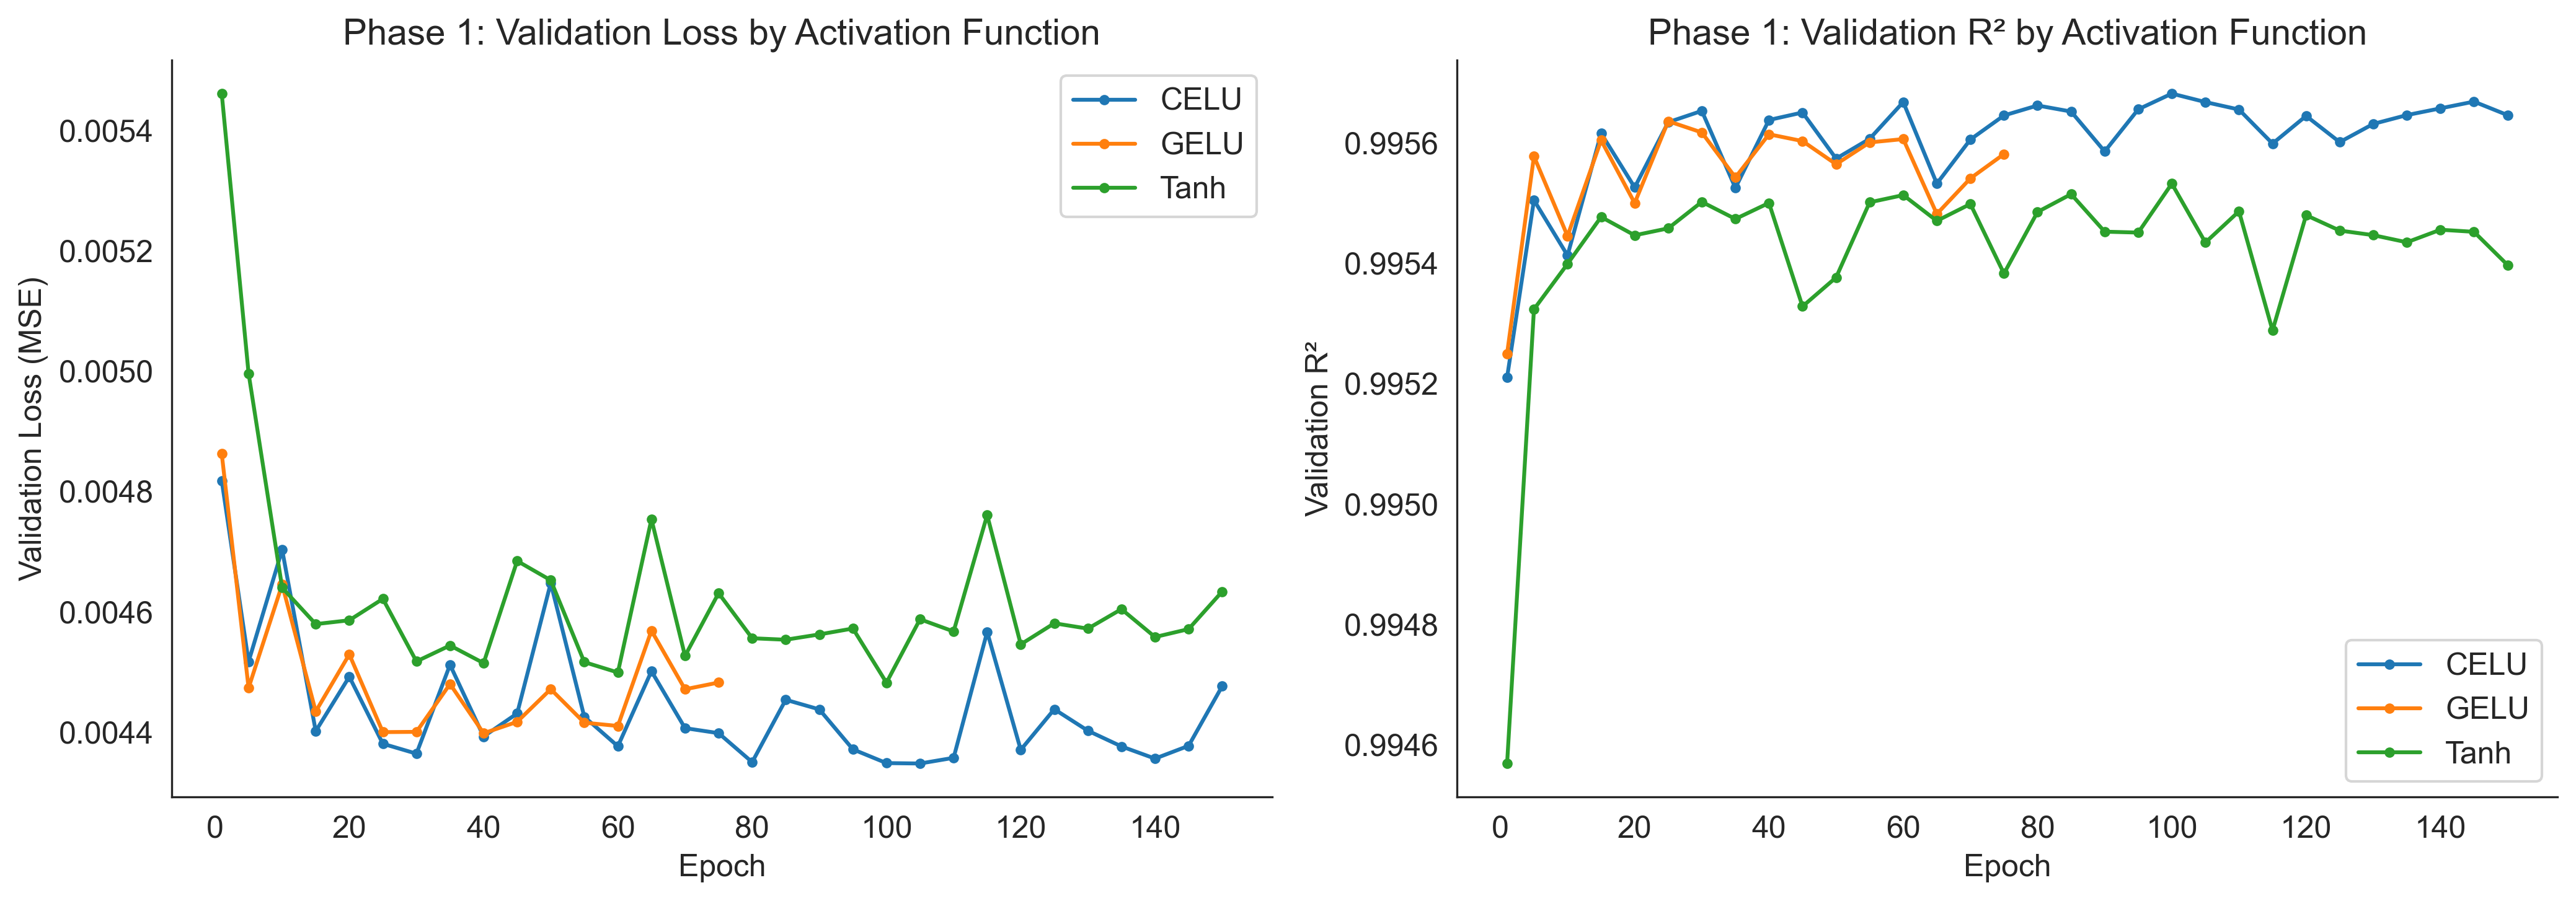
\includegraphics[width=0.95\textwidth]{Thesis/Chapter 4/Figures/fig_phase1_activation_comparison.png}
\caption{Phase~1: validation MSE loss (left) and validation $R^2$
(right) by activation function over training epochs.}
\label{fig:phase1_activation_ch4}
\end{figure}

\noindent
Figure~\ref{fig:phase1_activation_ch4} shows that \gls{celu} achieves
the lowest validation loss (approximately $0.00435$) and the highest
validation $R^2$ (approximately $0.9957$) from epoch~60 onwards. GELU
tracks \gls{celu} closely throughout training but settles at a
marginally higher loss plateau. Tanh converges more slowly and exhibits
greater epoch-to-epoch volatility, reaching a best validation $R^2$ of
approximately $0.9954$. The \gls{celu} activation was therefore retained.

\subsubsection{Phase 2: Learning rate}

Four learning rates were evaluated:
$\eta \in \{0.01, 0.001, 0.0005, 0.0001\}$, with \gls{celu} carried
forward.

\begin{figure}[H]
\centering
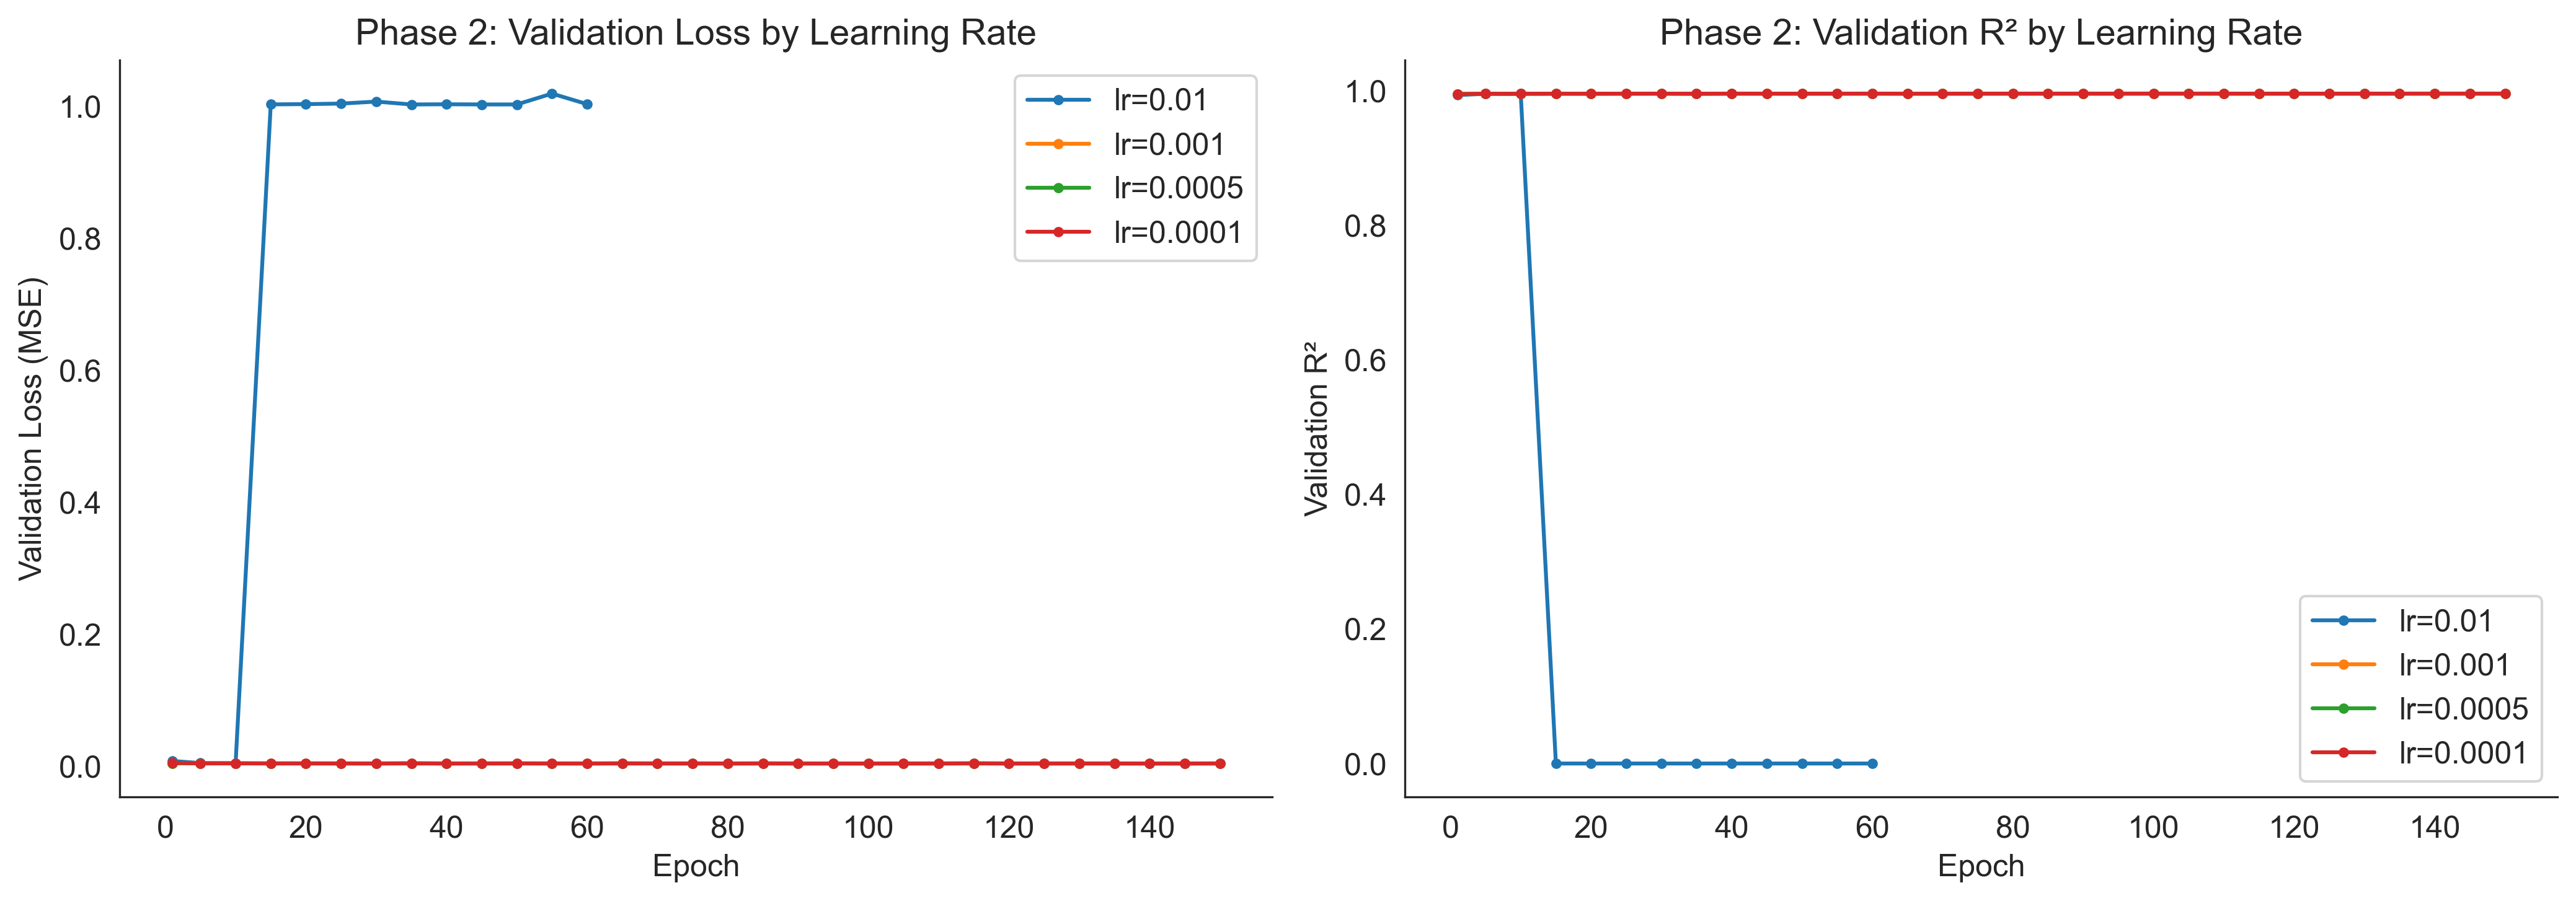
\includegraphics[width=0.95\textwidth]{Thesis/Chapter 4/Figures/fig_phase2_lr_comparison.png}
\caption{Phase~2: validation MSE loss (left) and validation $R^2$
(right) by learning rate.}
\label{fig:phase2_lr_ch4}
\end{figure}

\noindent
Figure~\ref{fig:phase2_lr_ch4} reveals that $\eta = 0.01$ produces
catastrophic divergence: the validation loss exceeds $1.0$ and the
validation $R^2$ drops to near zero, indicating that the gradient
updates overshoot the loss surface at this step size. The three
remaining learning rates ($0.001$, $0.0005$ and $0.0001$) all converge
to validation $R^2 \approx 1.00$ on the standardised scale, with their
loss curves overlapping on the visible scale. Among these,
$\eta = 0.0005$ achieves the lowest best validation loss and was
retained.

\subsubsection{Phase 3: Batch size}

Four batch sizes were compared:
$|\mathcal{B}| \in \{64, 128, 256, 512\}$, with \gls{celu} and
$\eta = 0.0005$ fixed.

\begin{figure}[H]
\centering
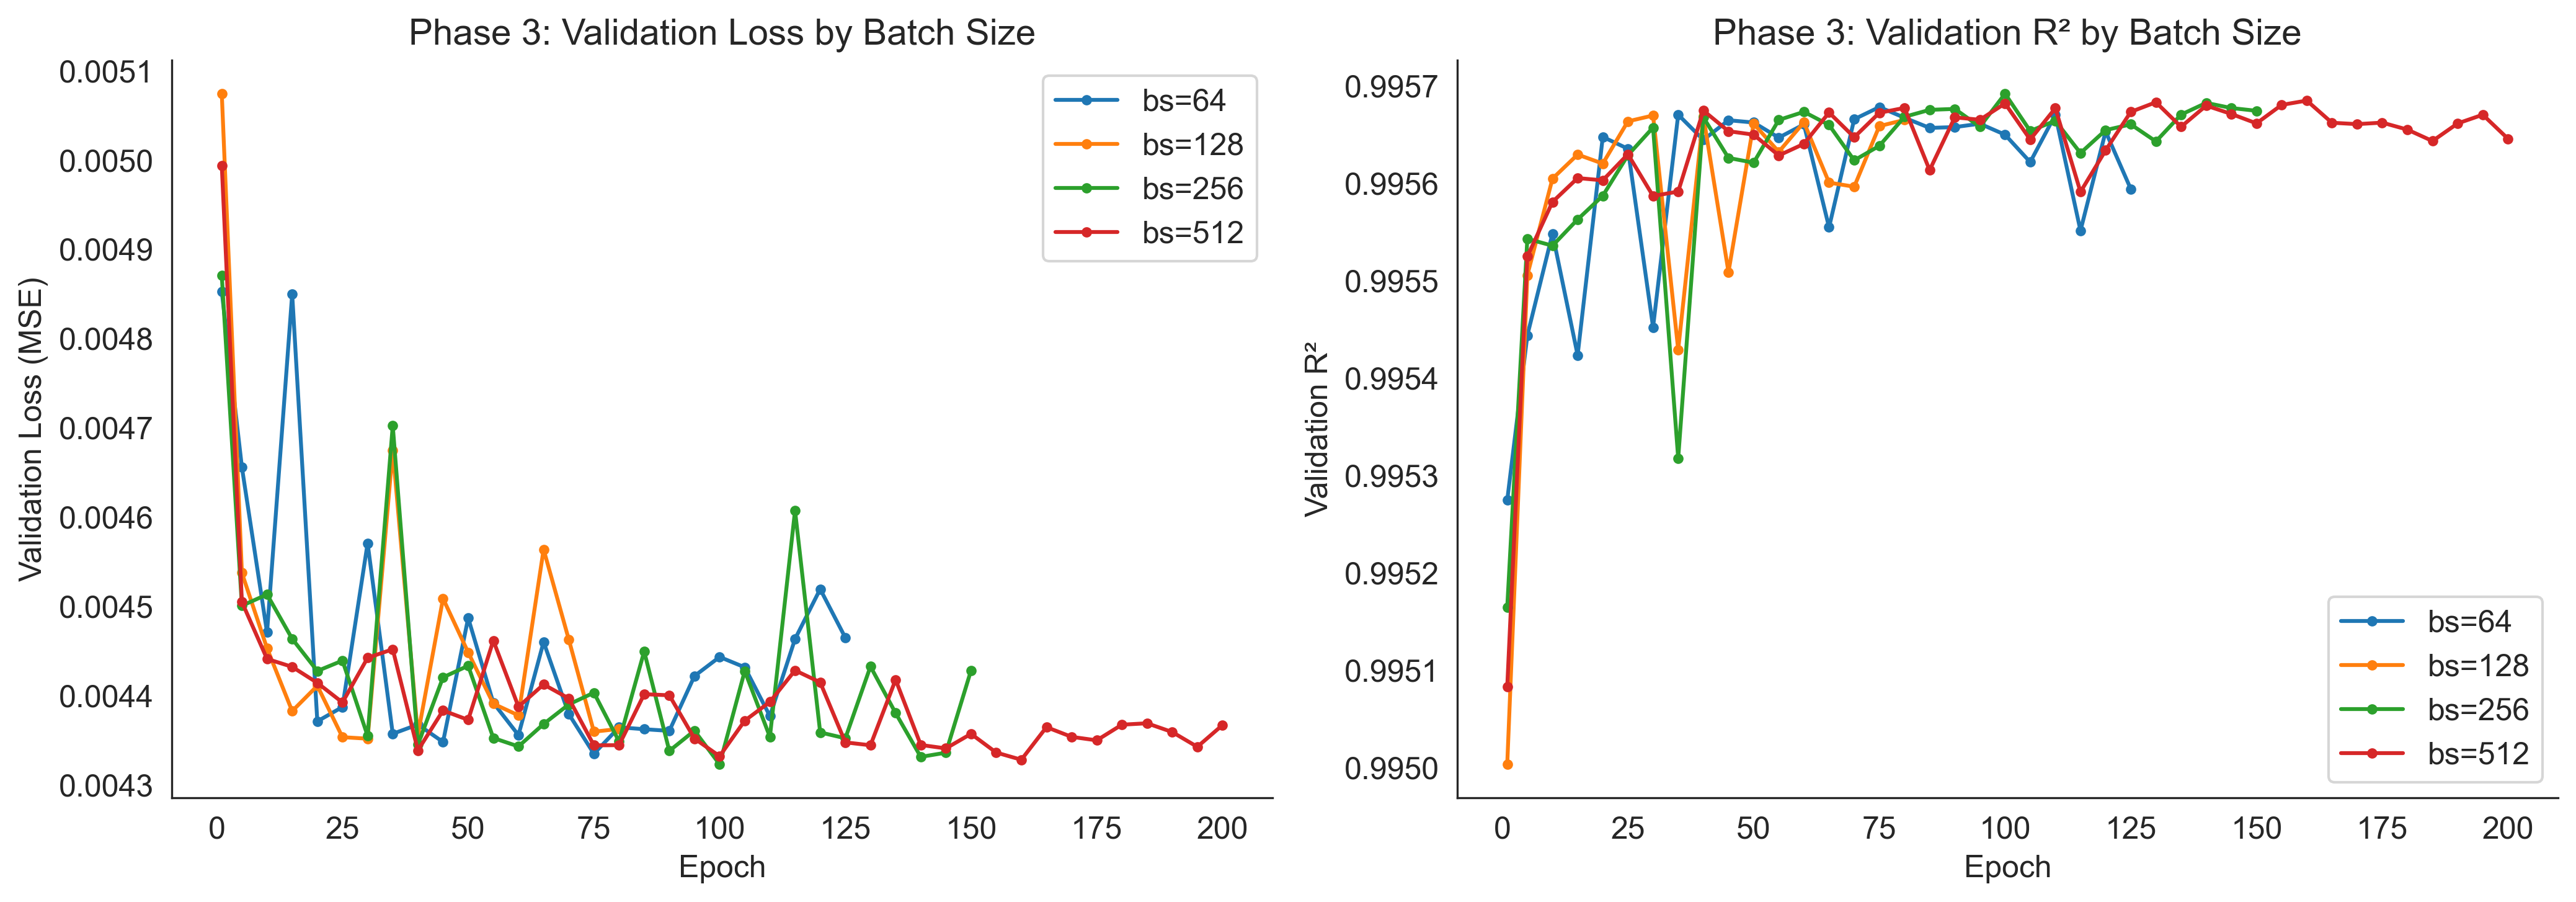
\includegraphics[width=0.95\textwidth]{Thesis/Chapter 4/Figures/fig_phase3_batchsize_comparison.png}
\caption{Phase~3: validation MSE loss (left) and validation $R^2$
(right) by batch size.}
\label{fig:phase3_batchsize_ch4}
\end{figure}

\noindent
Figure~\ref{fig:phase3_batchsize_ch4} shows that all four batch sizes
converge to similar validation performance, with best validation $R^2$
values between $0.9956$ and $0.9957$. The batch size $|\mathcal{B}| =
256$ was retained, as it achieves among the lowest validation loss
values while maintaining stable convergence behaviour.

\subsubsection{Phase 4: Optimiser}

Adam and Nadam were compared with all previous best choices carried
forward.

\begin{figure}[H]
\centering
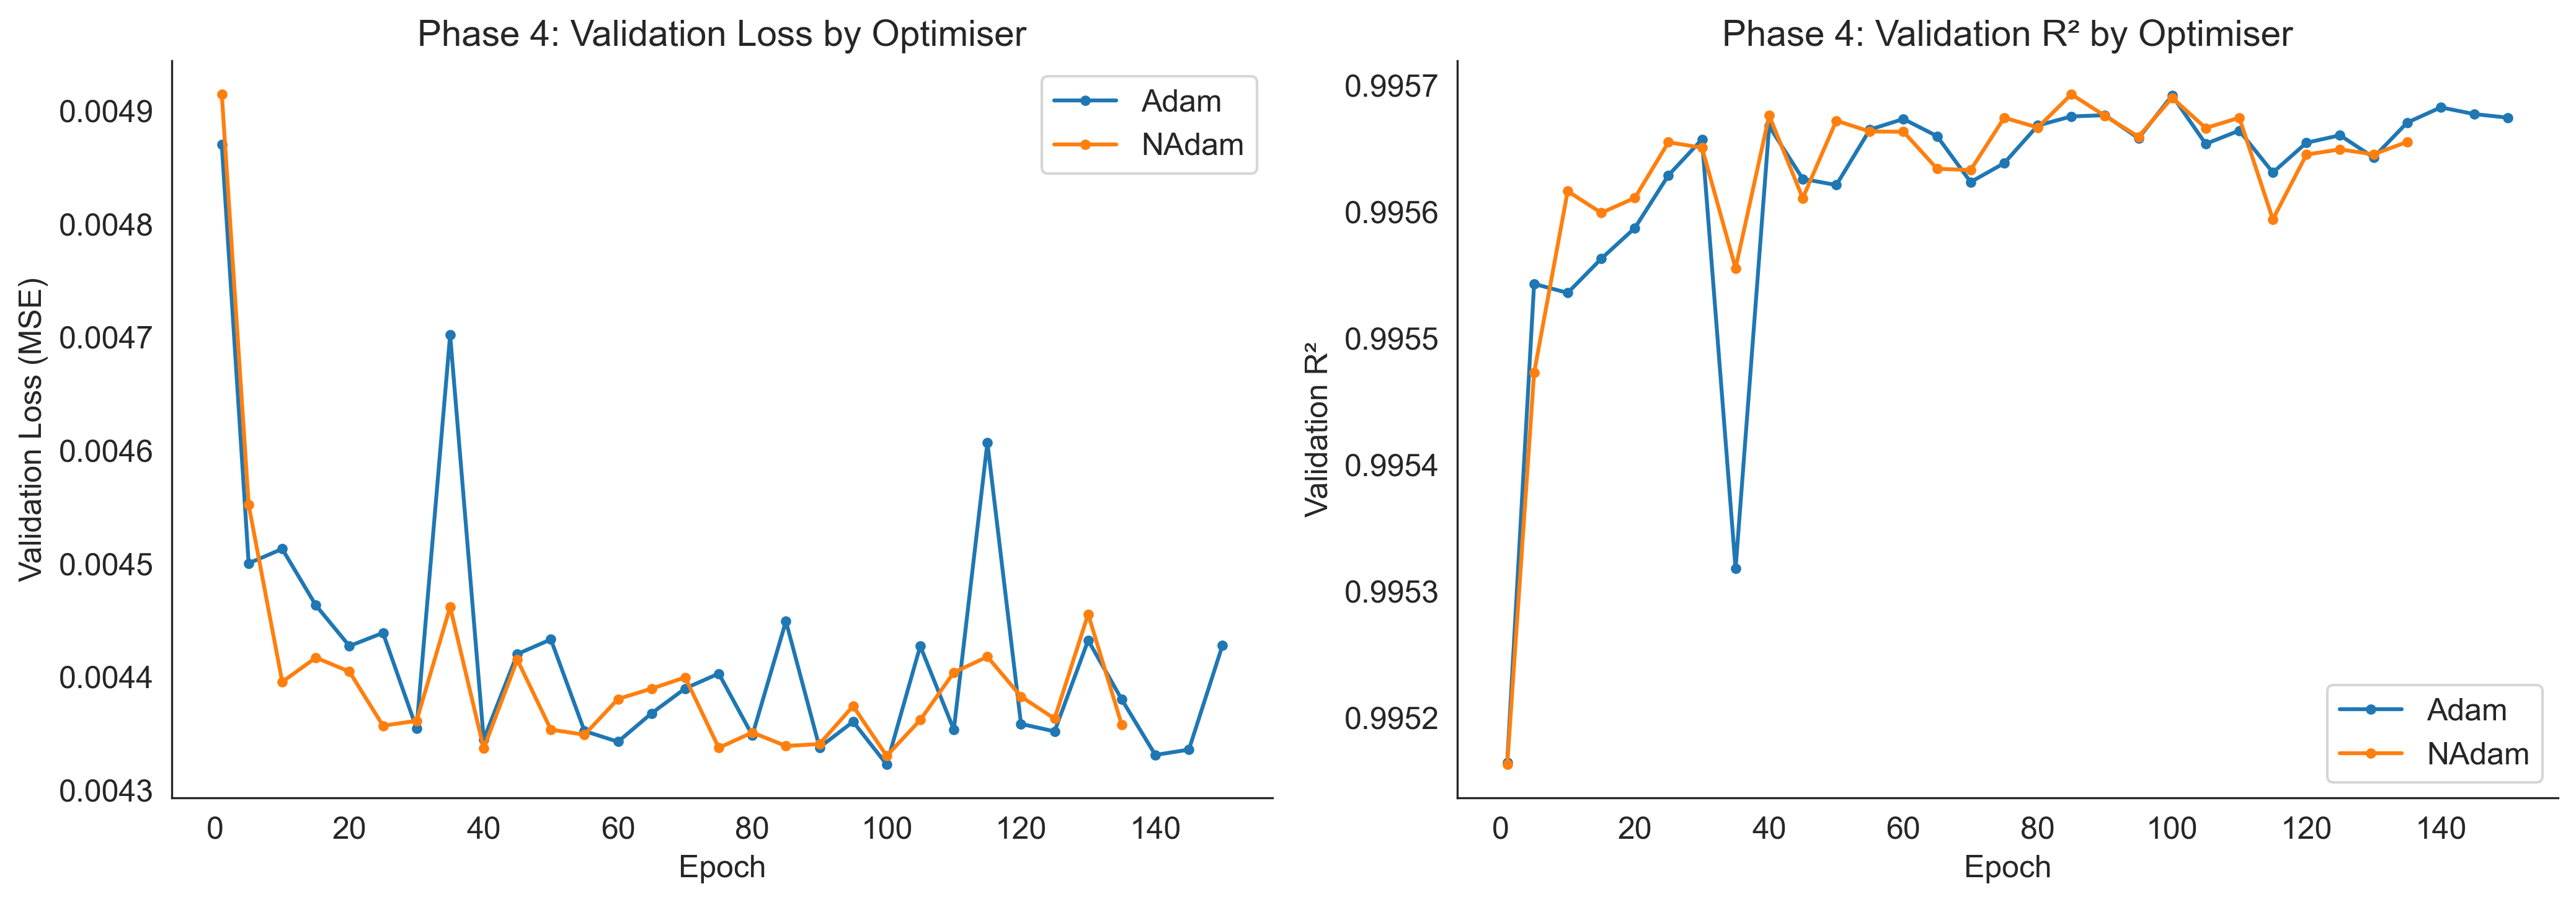
\includegraphics[width=0.95\textwidth]{Thesis/Chapter 4/Figures/fig_phase4_optimiser_comparison.png}
\caption{Phase~4: validation MSE loss (left) and validation $R^2$
(right) by optimiser.}
\label{fig:phase4_optimiser_ch4}
\end{figure}

\noindent
Figure~\ref{fig:phase4_optimiser_ch4} shows that Nadam converges faster
than Adam in the initial epochs and exhibits smoother validation loss
trajectories throughout training. From approximately epoch~40 onwards,
Nadam consistently achieves lower validation loss and higher validation
$R^2$ than Adam, with fewer loss spikes. Nadam was therefore retained.

\subsubsection{Phase 5: Momentum parameters}

Three momentum configurations were compared for the Nadam optimiser:
$(\beta_1, \beta_2) \in \{(0.90, 0.999),\; (0.95, 0.999),\;
(0.99, 0.999)\}$.

\begin{figure}[H]
\centering
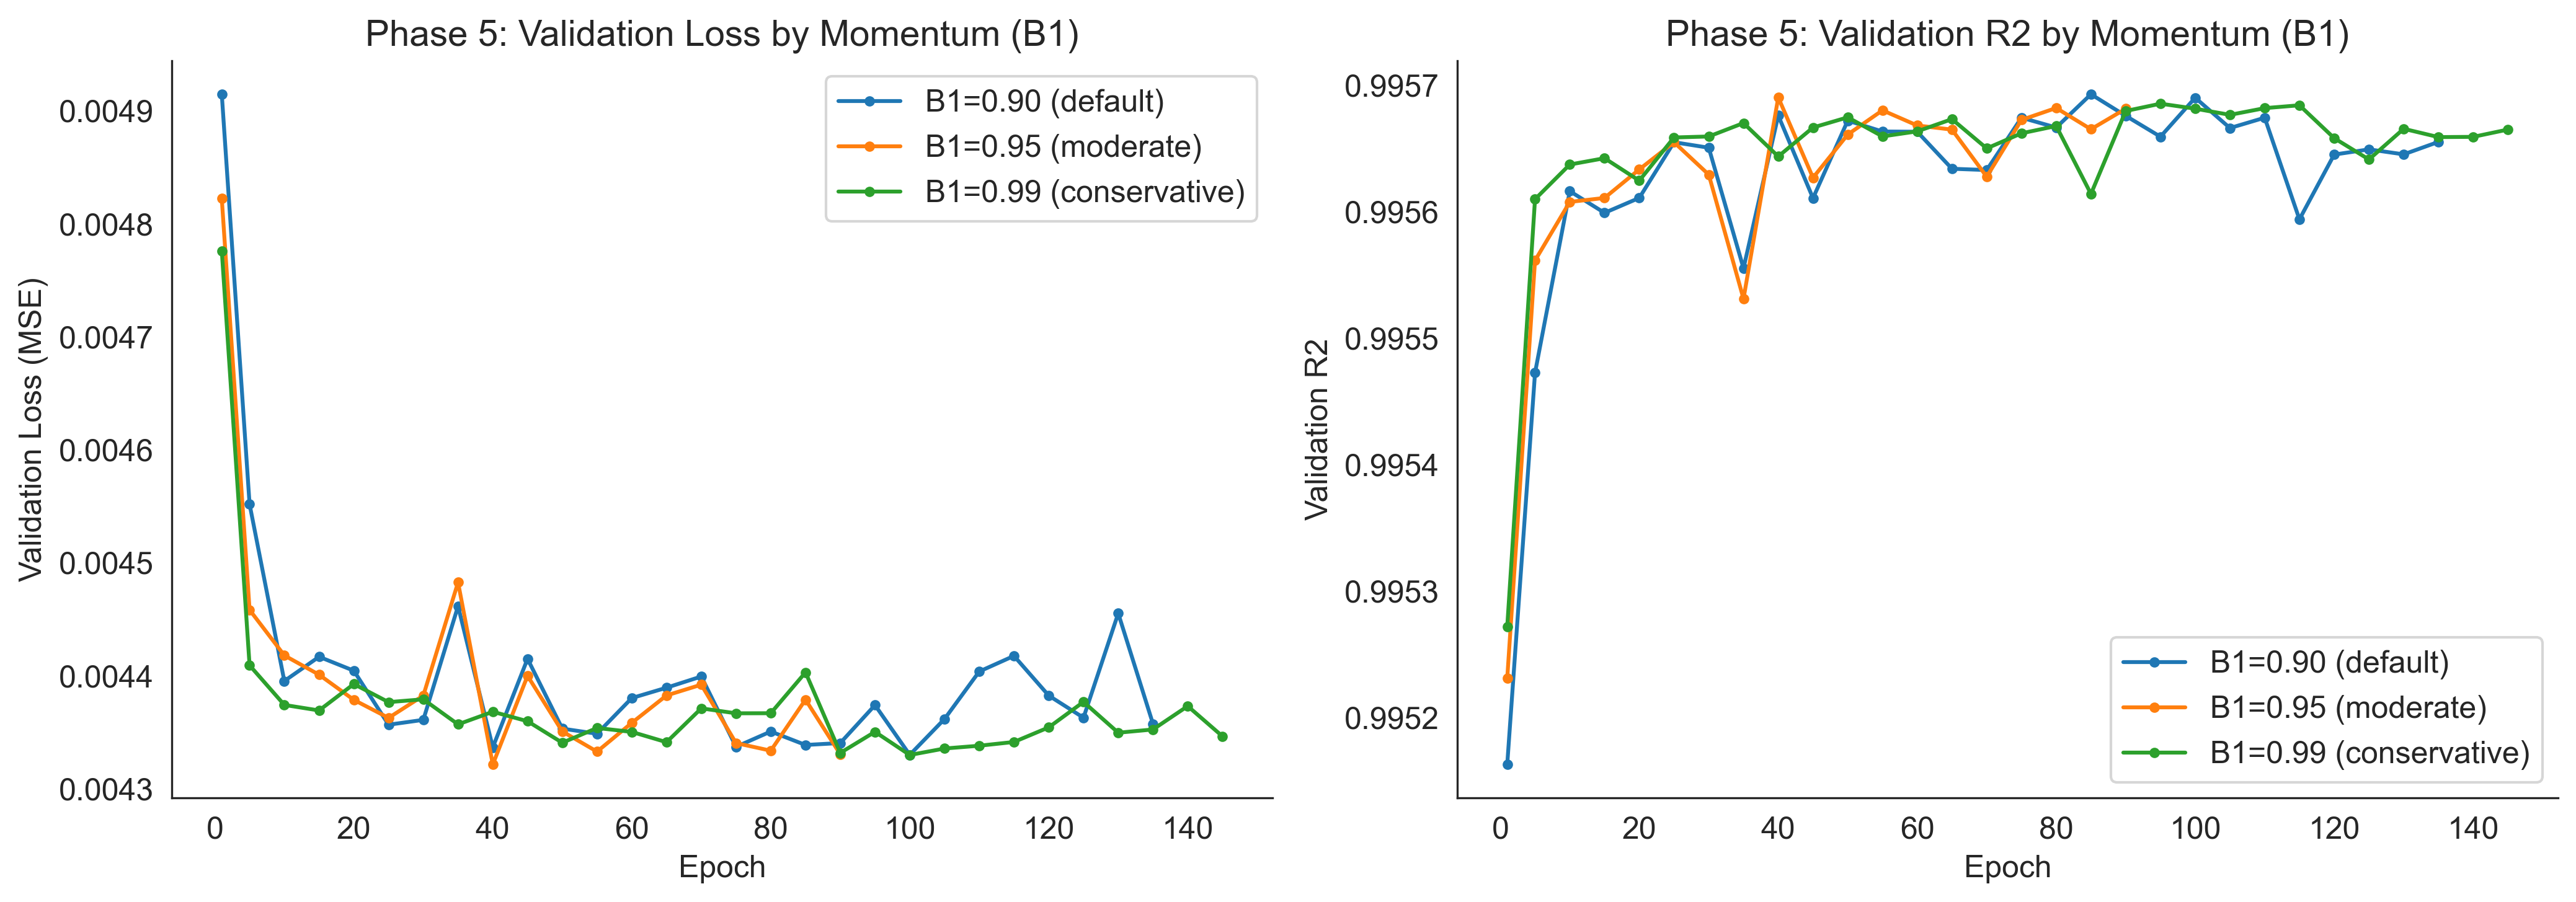
\includegraphics[width=0.95\textwidth]{Thesis/Chapter 4/Figures/fig_phase5_momentum_comparison.png}
\caption{Phase~5: validation MSE loss (left) and validation $R^2$
(right) by first momentum coefficient $\beta_1$.}
\label{fig:phase5_momentum_ch4}
\end{figure}

\noindent
Figure~\ref{fig:phase5_momentum_ch4} shows that all three momentum
configurations converge to similar final validation performance. The
$\beta_1 = 0.95$ configuration achieves marginally lower and more
stable validation loss from epoch~40 onwards, with the best validation
$R^2$ reaching approximately $0.9957$. The conservative setting
$\beta_1 = 0.99$ converges slightly faster in early epochs but exhibits
comparable final performance. The configuration $(\beta_1, \beta_2) =
(0.95, 0.999)$ was retained.

\subsubsection{Hyperparameter comparison overview}

Figure~\ref{fig:validation_loss_overview_ch4} presents the best
validation loss achieved by each configuration across all five phases.

\begin{figure}[H]
\centering
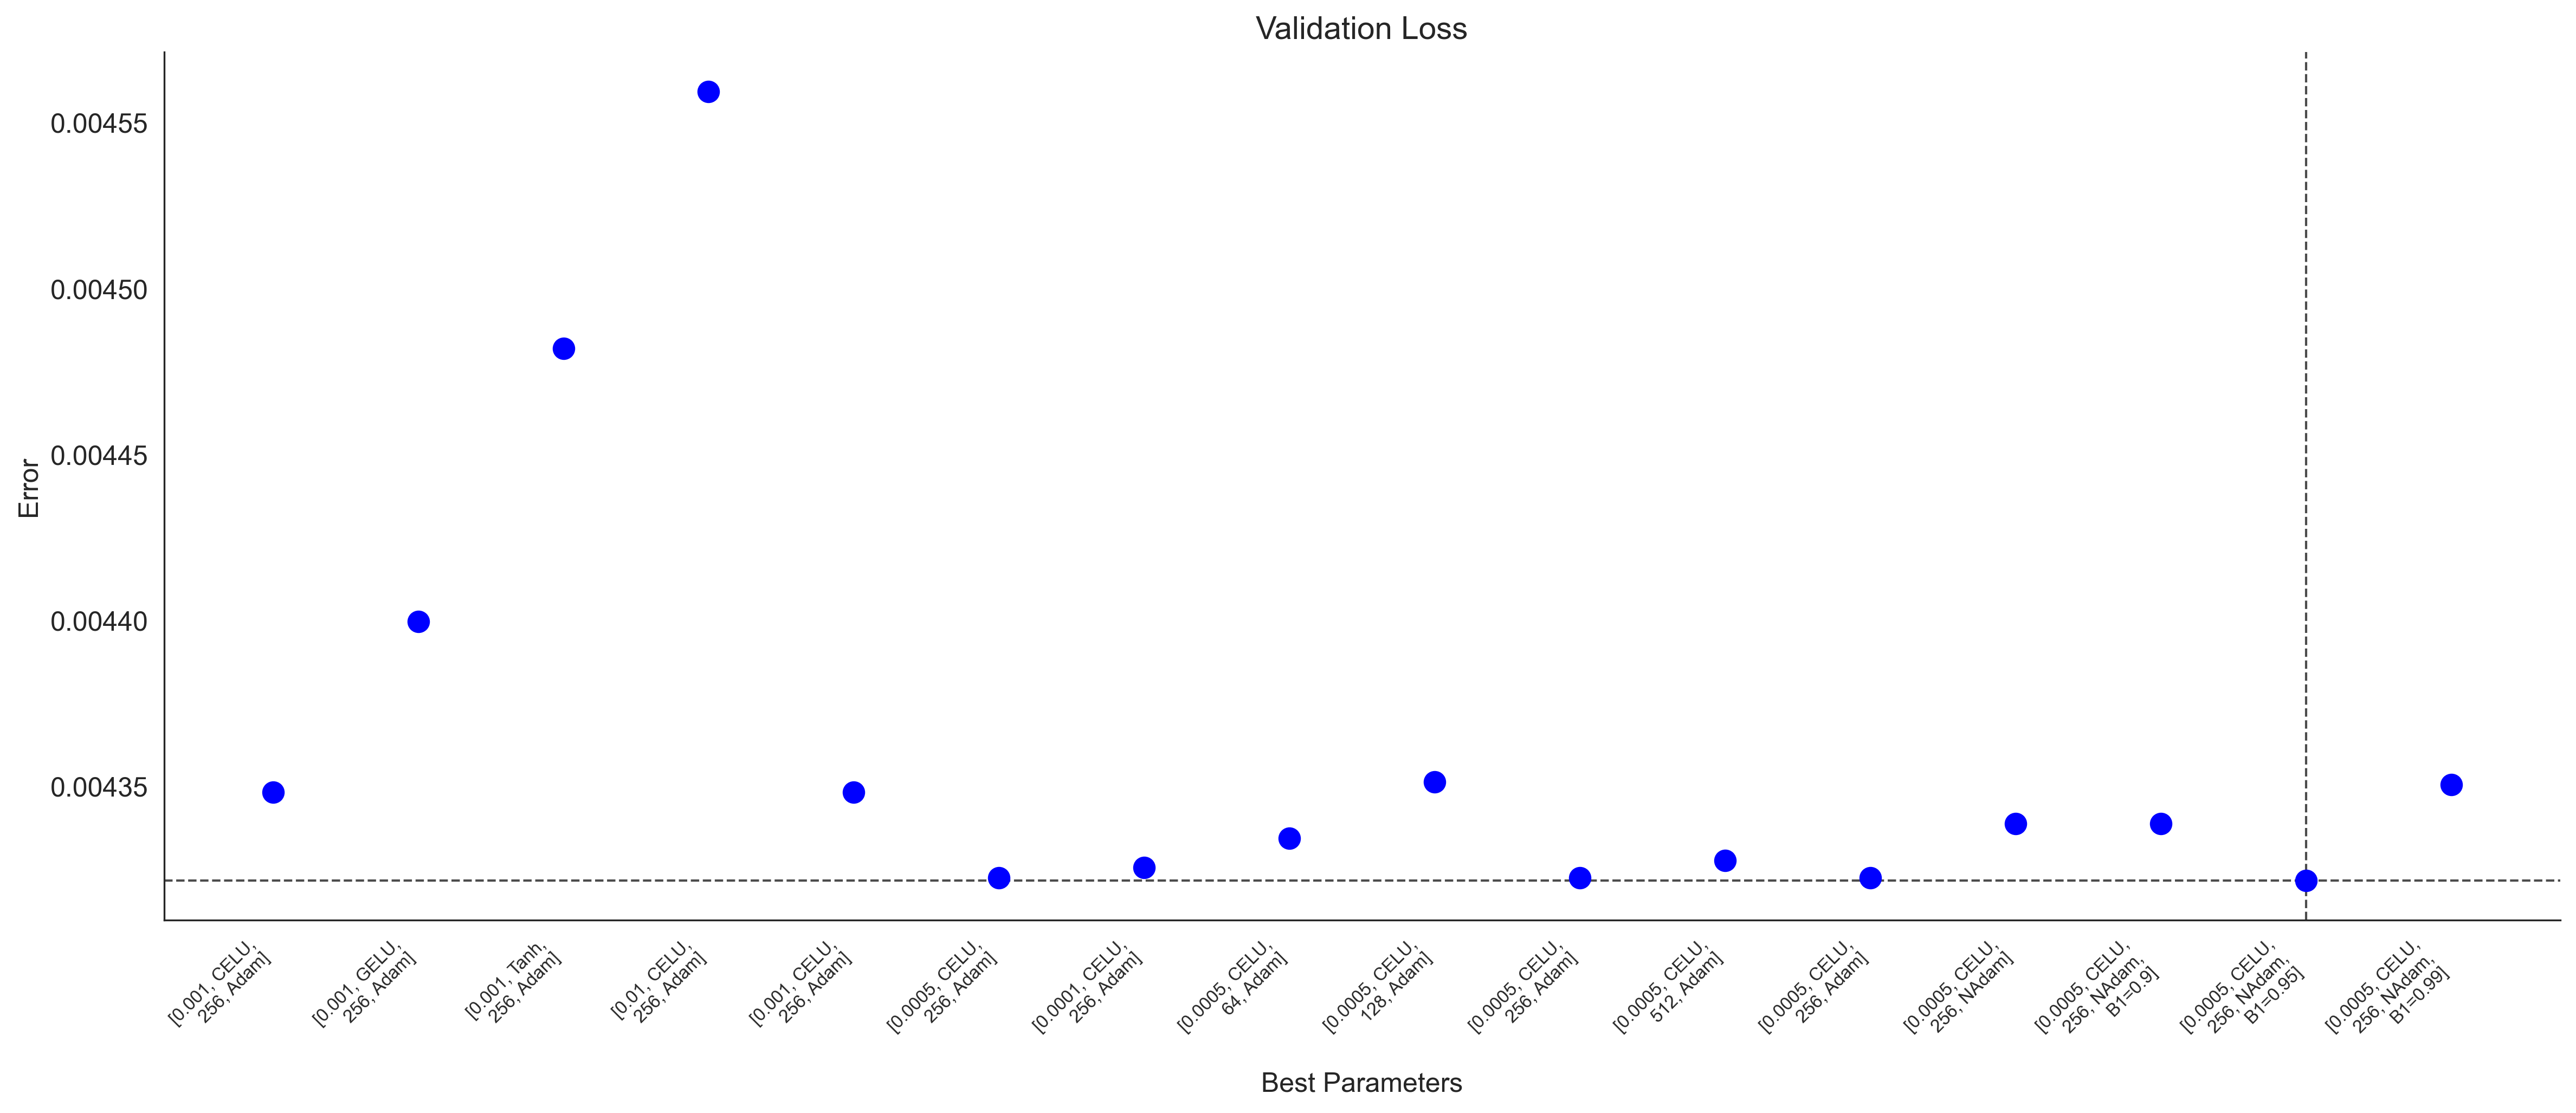
\includegraphics[width=0.95\textwidth]{Thesis/Chapter 4/Figures/fig_validation_loss_hyperparameters.png}
\caption{Best validation MSE loss across all hyperparameter
configurations evaluated in Phases~1-5.}
\label{fig:validation_loss_overview_ch4}
\end{figure}

\noindent
The selected configuration (CELU, $\eta = 0.0005$,
$|\mathcal{B}| = 256$, Nadam, $\beta_1 = 0.95$) achieves the lowest
validation loss among all evaluated configurations.
Table~\ref{tab:final_hyperparameters_ch4} records the final training
configuration.

\begin{table}[H]
\centering
\caption{Selected hyperparameters from the sequential comparison.}
\label{tab:final_hyperparameters_ch4}
\small
\renewcommand{\arraystretch}{1.15}
\begin{tabular}{p{0.30\textwidth}p{0.25\textwidth}p{0.30\textwidth}}
\toprule
\textbf{Phase} & \textbf{Candidates} & \textbf{Selected} \\
\midrule
1. Activation function & CELU, GELU, Tanh & CELU \\
2. Learning rate & 0.01, 0.001, 0.0005, 0.0001 & 0.0005 \\
3. Batch size & 64, 128, 256, 512 & 256 \\
4. Optimiser & Adam, Nadam & Nadam \\
5. Momentum $(\beta_1, \beta_2)$ & (0.90, 0.999), (0.95, 0.999), (0.99, 0.999) & (0.95, 0.999) \\
\bottomrule
\end{tabular}
\end{table}

\subsubsection{Final model predictive performance}

The final \gls{dnn} was retrained with the selected configuration and
early stopping at epoch $e^{*} = 85$ (the checkpoint with the highest
validation $R^2$).
Table~\ref{tab:final_model_performance_ch4} reports the predictive
performance metrics computed on the original monetary scale after
de-normalising the fitted predictions, using the \gls{mae}
(equation~\eqref{eq:mae}), \gls{rmse} (equation~\eqref{eq:rmse}), and
$R^2$ (equation~\eqref{eq:r_squared}).

\begin{table}[H]
\centering
\caption{Predictive performance of the final DNN on the original
monetary scale.}
\label{tab:final_model_performance_ch4}
\small
\renewcommand{\arraystretch}{1.15}
\begin{tabular}{lrrr}
\toprule
\textbf{Partition} & \textbf{MAE (R)} & \textbf{RMSE (R)} & $\boldsymbol{R^2}$ \\
\midrule
Training ($n = 524\,288$) & 251 & 291 & 0.9957 \\
Test ($n = 237\,856$) & 251 & 290 & 0.9957 \\
\bottomrule
\end{tabular}
\end{table}

\noindent
The near-identical performance across partitions (MAE = R251 on both;
RMSE within R290 to R291; $R^2 = 0.9957$ on both) confirms that the
fitted model generalises to unseen data without overfitting.  The
training-set response statistics used for standardisation are
$\overline{y}_{\mathrm{train}} = \text{R16\,744}$ and
$s_{y,\mathrm{train}} = \text{R4\,419}$.  On the standardised scale,
the validation MSE at the selected epoch $e^{*} = 85$ is $0.00432$
(Figure~\ref{fig:validation_loss_overview_ch4}), and the
original-scale residuals range from approximately $-600$ to $+600$ as
characterised in the residual diagnostics of
Section~\ref{sec:model_validation_diagnostics}.

The model's predictive performance supports its use in the
subsequent simulation and attribution analyses.

\subsubsection{Baseline comparison: GLM (Gamma, log-link) versus DNN}
\label{sec:glm_vs_dnn_comparison_ch4}

The \gls{glm} benchmark specified in
Section~\ref{sec:glm_benchmark_methods} was evaluated alongside the
\gls{dnn}.  Table~\ref{tab:glm_vs_dnn_comparison_ch4} reports the
performance of both models across training, validation and test
partitions.

\begin{table}[H]
\centering
\caption{Predictive performance comparison: \gls{glm} (Gamma, log-link)
versus \gls{dnn} (funnel architecture) on the original monetary scale.}
\label{tab:glm_vs_dnn_comparison_ch4}
\small
\renewcommand{\arraystretch}{1.15}
\begin{tabular}{llrrr}
\toprule
\textbf{Model} & \textbf{Partition} & \textbf{MAE (R)} &
\textbf{RMSE (R)} & $\boldsymbol{R^2}$ \\
\midrule
\gls{glm} (Gamma, log-link)
    & Training   & 623 & 911 & 0.9574 \\
    & Validation & 622 & 913 & 0.9574 \\
    & Test       & 624 & 913 & 0.9571 \\
\addlinespace
\gls{dnn} (Funnel)
    & Training   & 251 & 291 & 0.9957 \\
    & Validation & 251 & 291 & 0.9957 \\
    & Test       & 251 & 290 & 0.9957 \\
\bottomrule
\end{tabular}
\end{table}

\noindent
The \gls{dnn} outperforms the \gls{glm} on every metric.  On the test
set, the \gls{dnn} achieves an $R^2$ of $0.9957$ compared with
$0.9571$ for the \gls{glm}, an improvement of $3.86$ percentage points.
The test \gls{rmse} decreases from R913 to R290 (a $68.2\%$ reduction),
and the test \gls{mae} decreases from R624 to R251 (a $59.8\%$
reduction).

\begin{figure}[H]
\centering
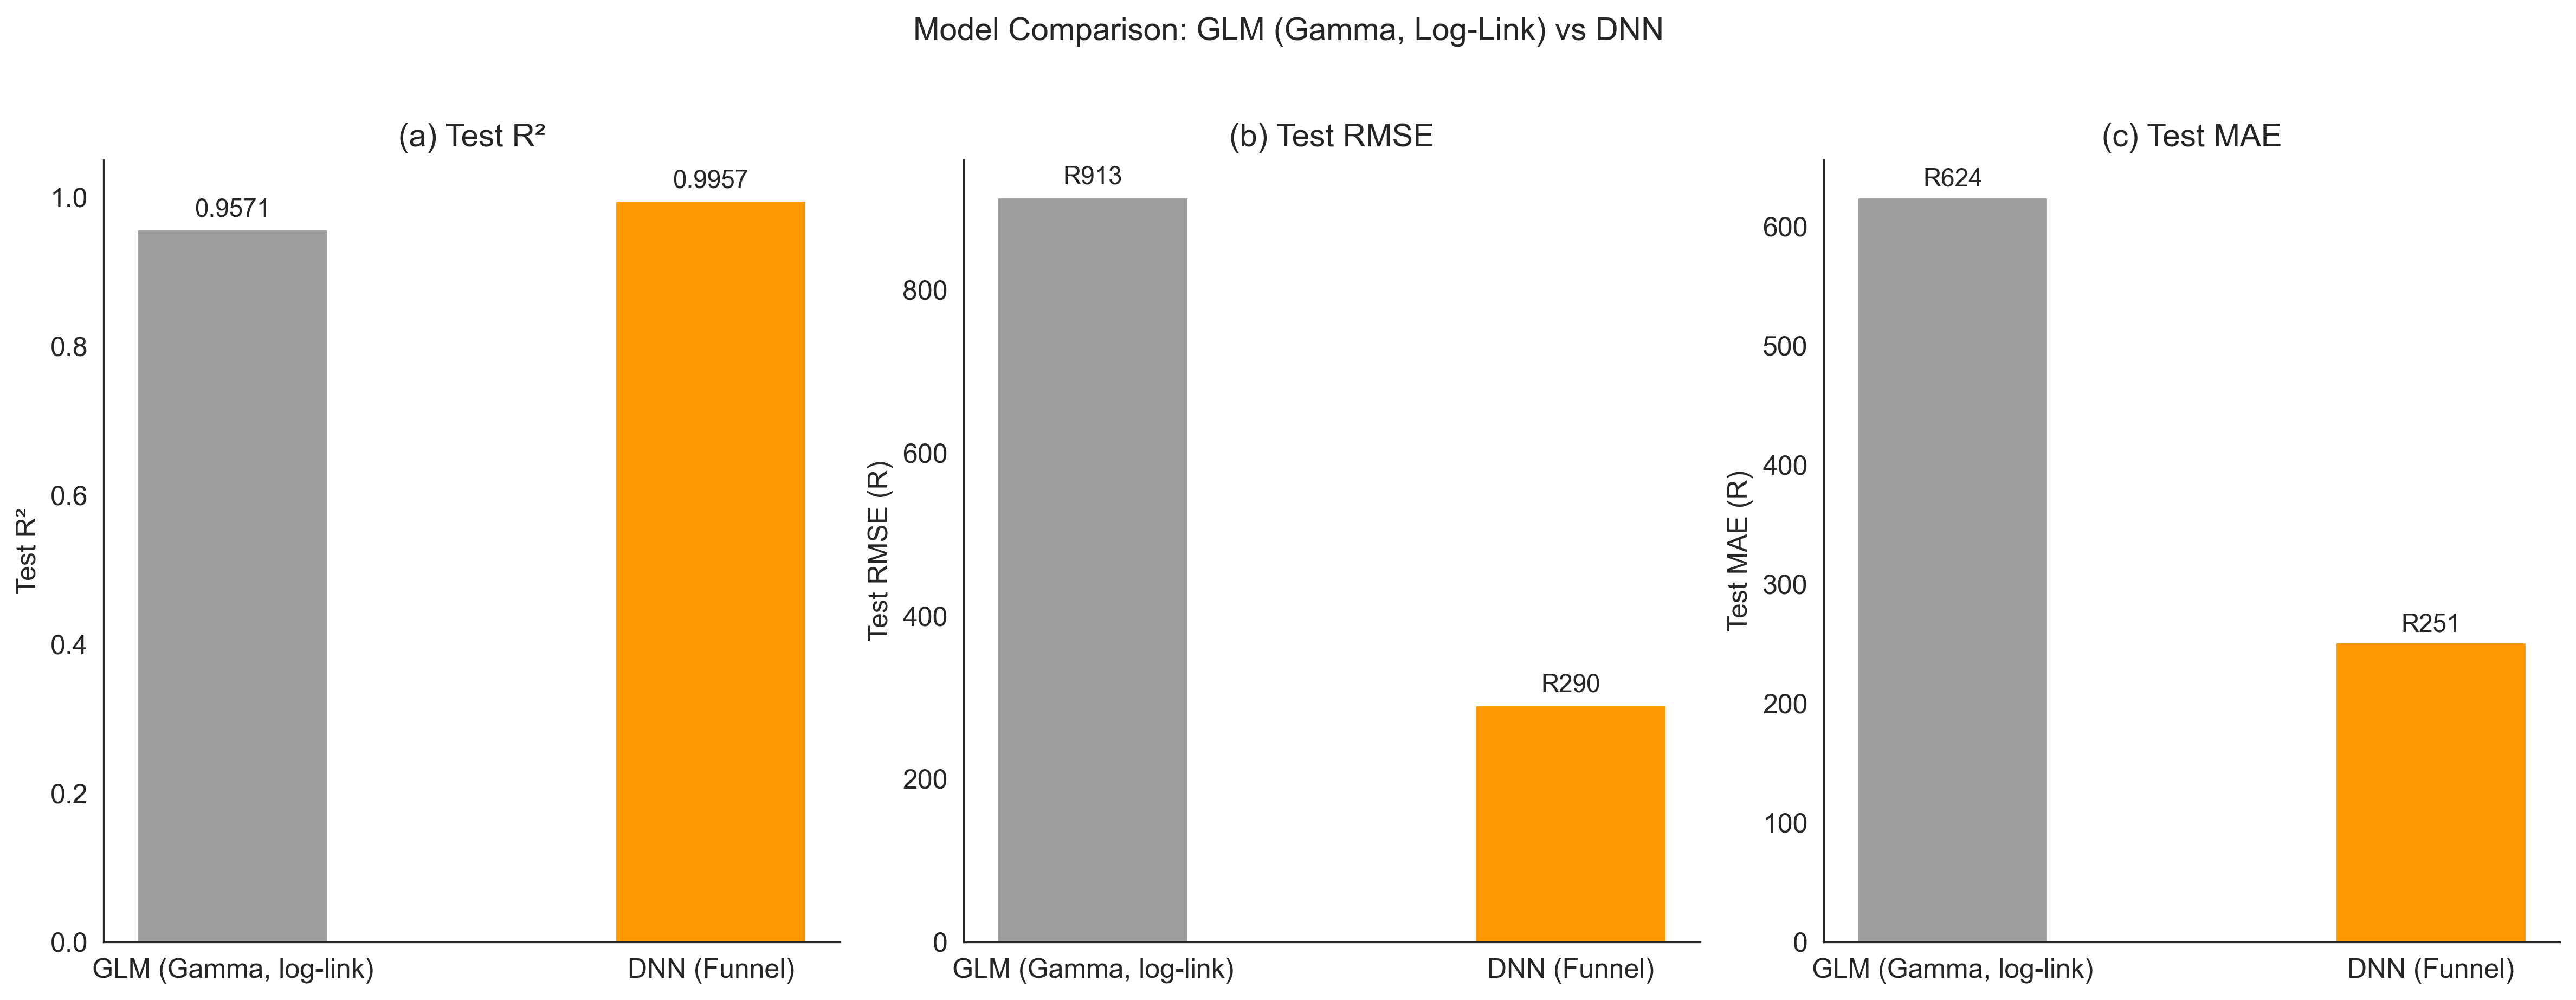
\includegraphics[width=0.95\textwidth]{Thesis/Chapter 4/Figures/fig_glm_vs_dnn_comparison.png}
\caption{Test-set performance comparison: \gls{glm} (Gamma, log-link)
versus \gls{dnn}.  (a)~Test $R^2$; (b)~test RMSE; (c)~test MAE.}
\label{fig:glm_vs_dnn_comparison_ch4}
\end{figure}

\noindent
Figure~\ref{fig:glm_vs_dnn_comparison_ch4} visualises the test-set
comparison.  The \gls{glm}'s inferior fit is attributable to the
log-link's multiplicative mean structure, which does not match the
additive data-generating process underlying this dataset.  The charges
variable is constructed as an approximately linear function of the input
features plus noise; the \gls{glm}'s exponential inverse-link therefore
introduces systematic model misspecification.  The \gls{dnn}, by
contrast, learns the additive structure directly through its flexible
hidden-layer representations.

\begin{figure}[H]
\centering
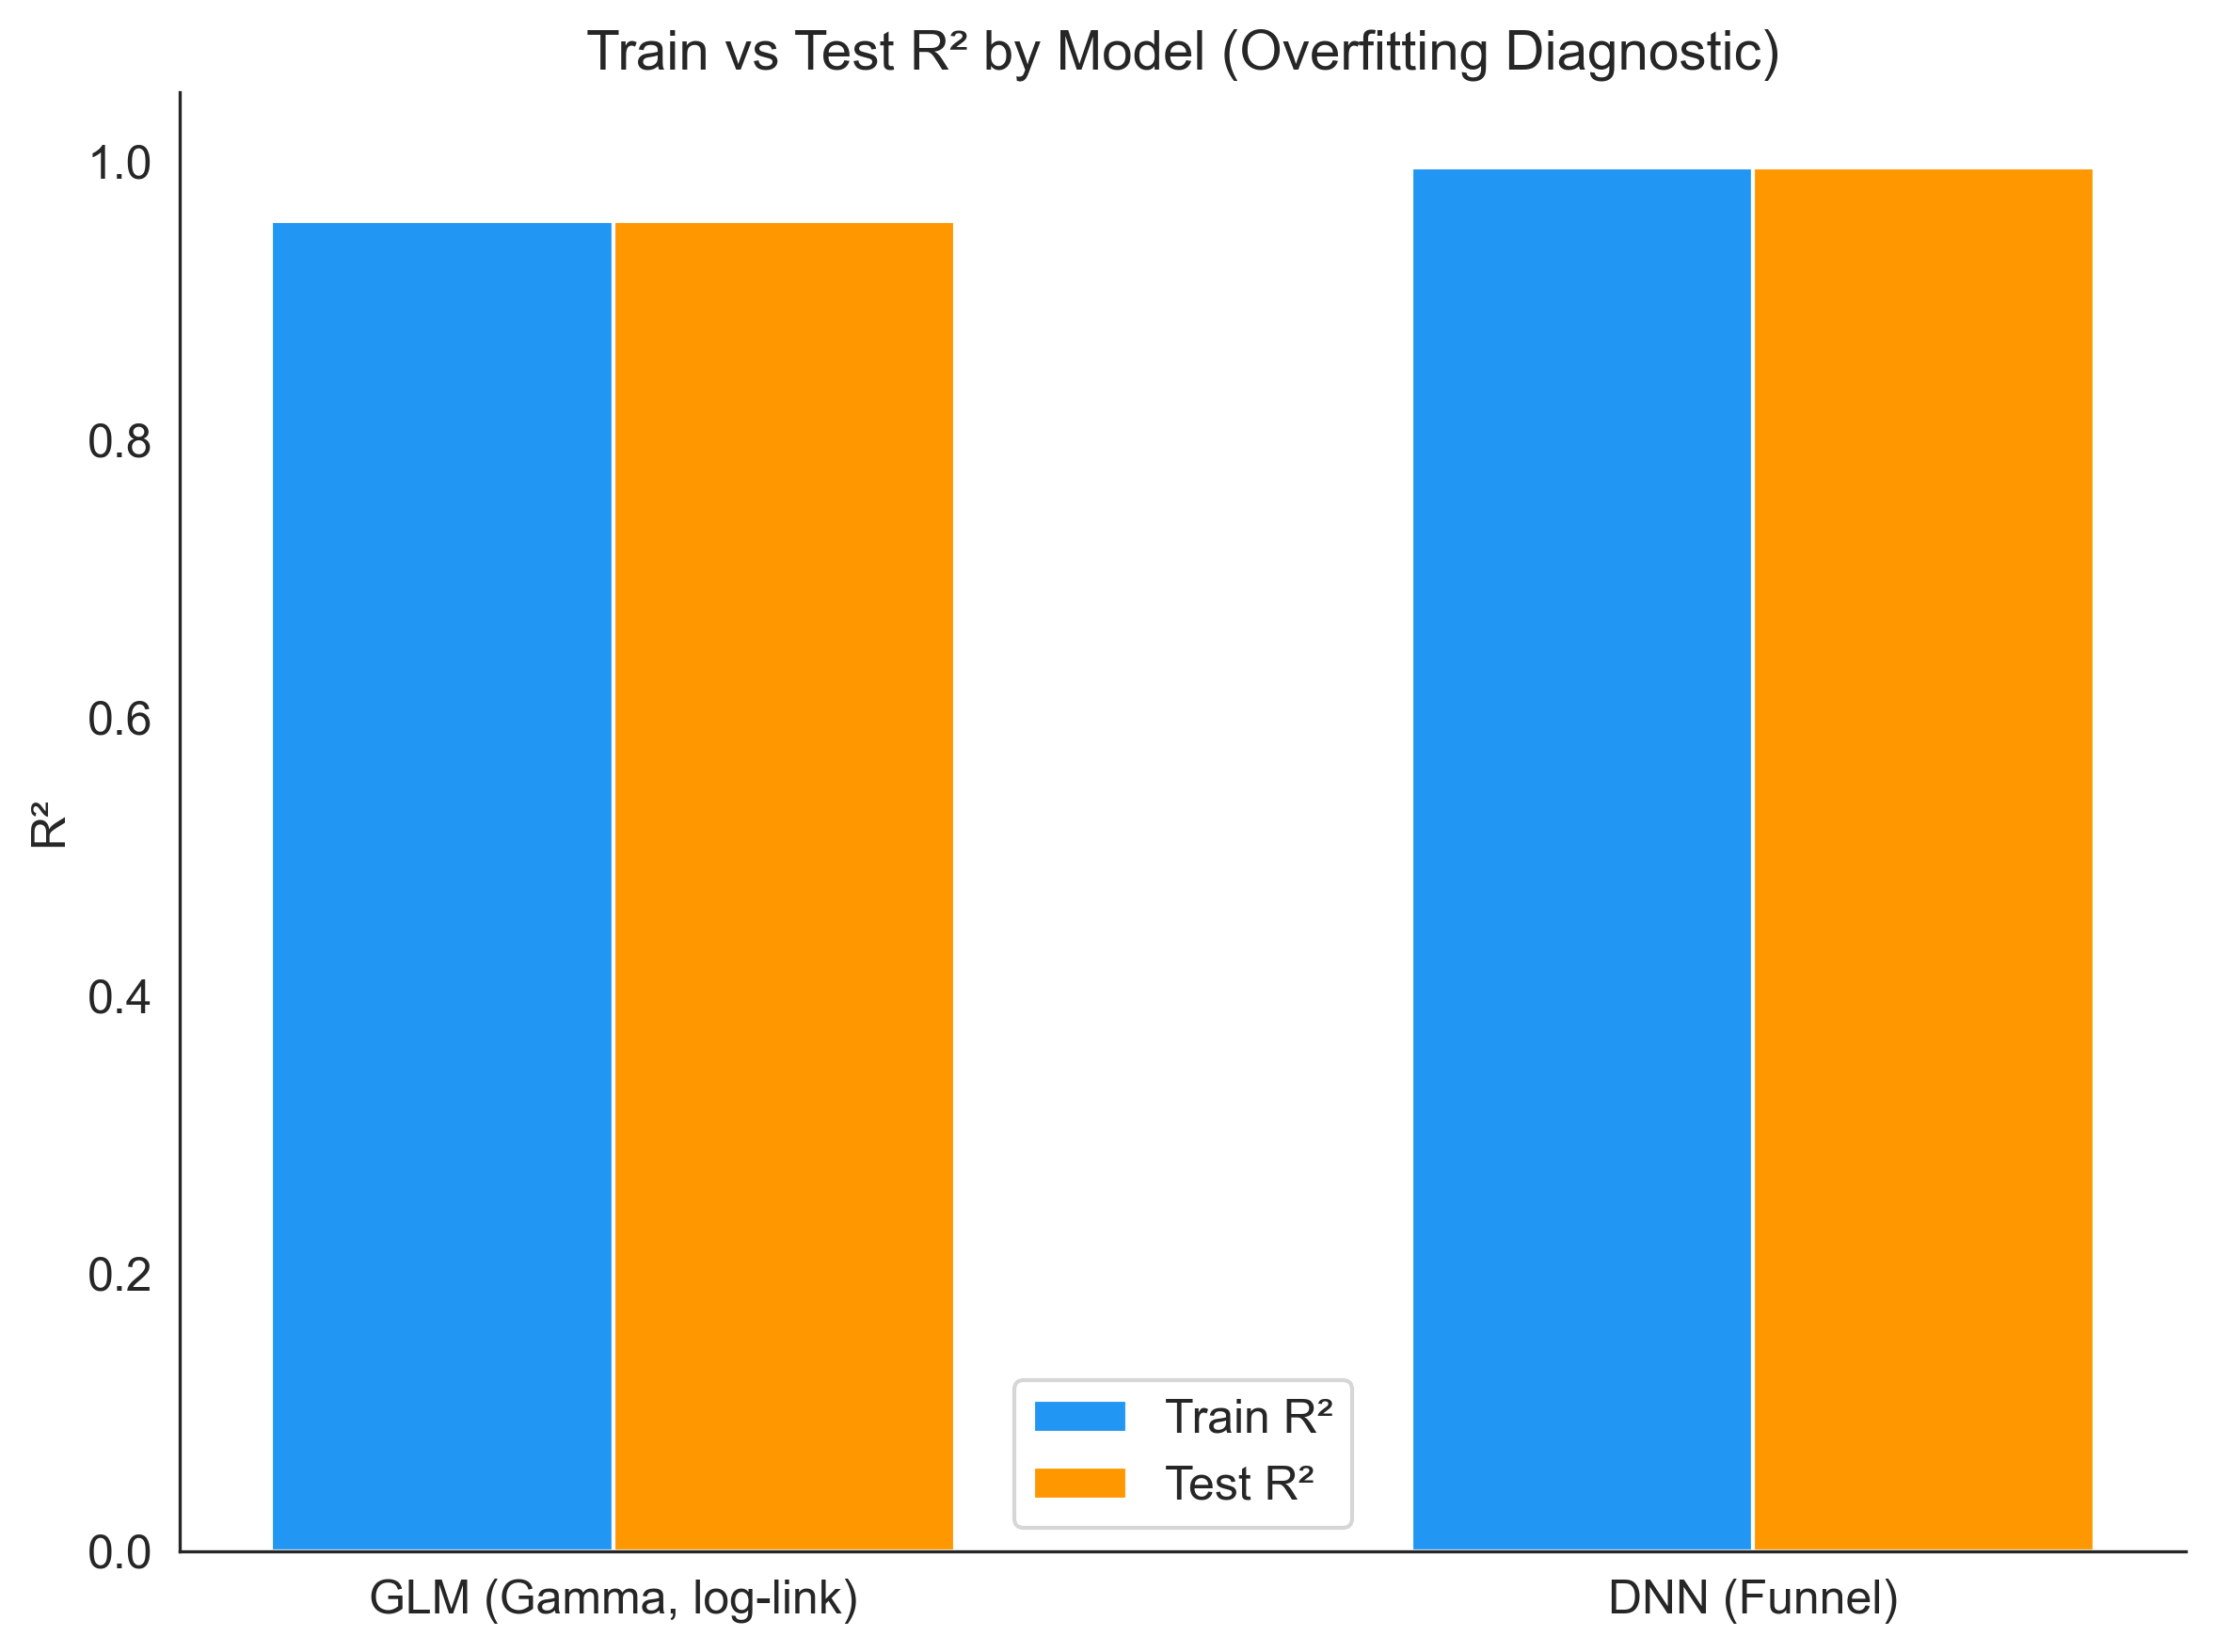
\includegraphics[width=0.65\textwidth]{Thesis/Chapter 4/Figures/fig_train_test_r2_overfitting.png}
\caption{Overfitting diagnostic: training versus test $R^2$ for both
models.}
\label{fig:train_test_r2_overfitting_ch4}
\end{figure}

\noindent
Figure~\ref{fig:train_test_r2_overfitting_ch4} compares the training
and test $R^2$ for both models.  The \gls{glm} shows negligible
generalisation loss ($R^2_{\mathrm{train}} = 0.9574$ versus
$R^2_{\mathrm{test}} = 0.9571$), as expected for a parametric model
with far fewer parameters than observations.  The \gls{dnn} likewise
shows no evidence of overfitting ($R^2_{\mathrm{train}} = 0.9957$
versus $R^2_{\mathrm{test}} = 0.9957$), confirming that the early
stopping criterion (Section~\ref{sec:dnn_specification_training})
effectively regularises the 49\,168 trainable parameters.

The \gls{glm} comparison serves two purposes.  First, it establishes
that the \gls{dnn}'s high $R^2$ reflects genuine predictive superiority
over the actuarial-standard model class, not merely an artefact of the
dataset's synthetic regularity.  Second, because the Gamma/log-link
\gls{glm} is the model an actuary would deploy as a first approach, the
comparison provides the practical benchmark context that situates the
\gls{dnn} within the actuarial modelling landscape.  The \gls{dnn} is therefore retained for the subsequent analyses
on the grounds of its superior accuracy and its differentiability
for gradient-based attribution.

The finding that a deep neural network outperforms a classical \gls{glm}
on this benchmark is consistent with the broader health-cost prediction
literature.  \citet{dreweboss2022deep} report that deep-learning models
achieve lower prediction error than standard actuarial models on claims
data, while \citet{samiuddin2023health} and \citet{kaushik2022machine}
similarly observe that neural-network architectures improve upon
traditional regression baselines for insurance cost estimation.  As noted
in Section~\ref{sec:integrating_dnn_mc_shapley}, however, this
superiority is not universal across all tabular insurance datasets
\citep{richman2021ai}, and the present comparison is limited to a single
classical baseline on a benchmark dataset with a strong synthetic
structure.


% =============================================================
\subsection{Monte Carlo Predicted-Cost Distribution}
\label{sec:mc_results}

The base parametric Monte Carlo simulation (Algorithm~3.1) was executed
with $B = 10\,000$ synthetic policyholder profiles drawn from the
product-marginal input distribution specified in
equation~\eqref{eq:raw_product_mc_distribution_ch3}. Each simulated
profile was preprocessed, scored through the fitted \gls{dnn}, and
de-normalised to the original monetary scale.

\subsubsection{Simulated input validation}
\label{sec:simulated_input_validation_ch4}

The simulated inputs were validated following the joint-distribution
diagnostic protocol in Section~\ref{sec:mc_input_validation}.

\subsubsection*{Joint distribution validation}

Three complementary diagnostics compare the bivariate and multivariate
dependence structure of the training data with that of the Monte Carlo
sample.

\begin{figure}[H]
\centering
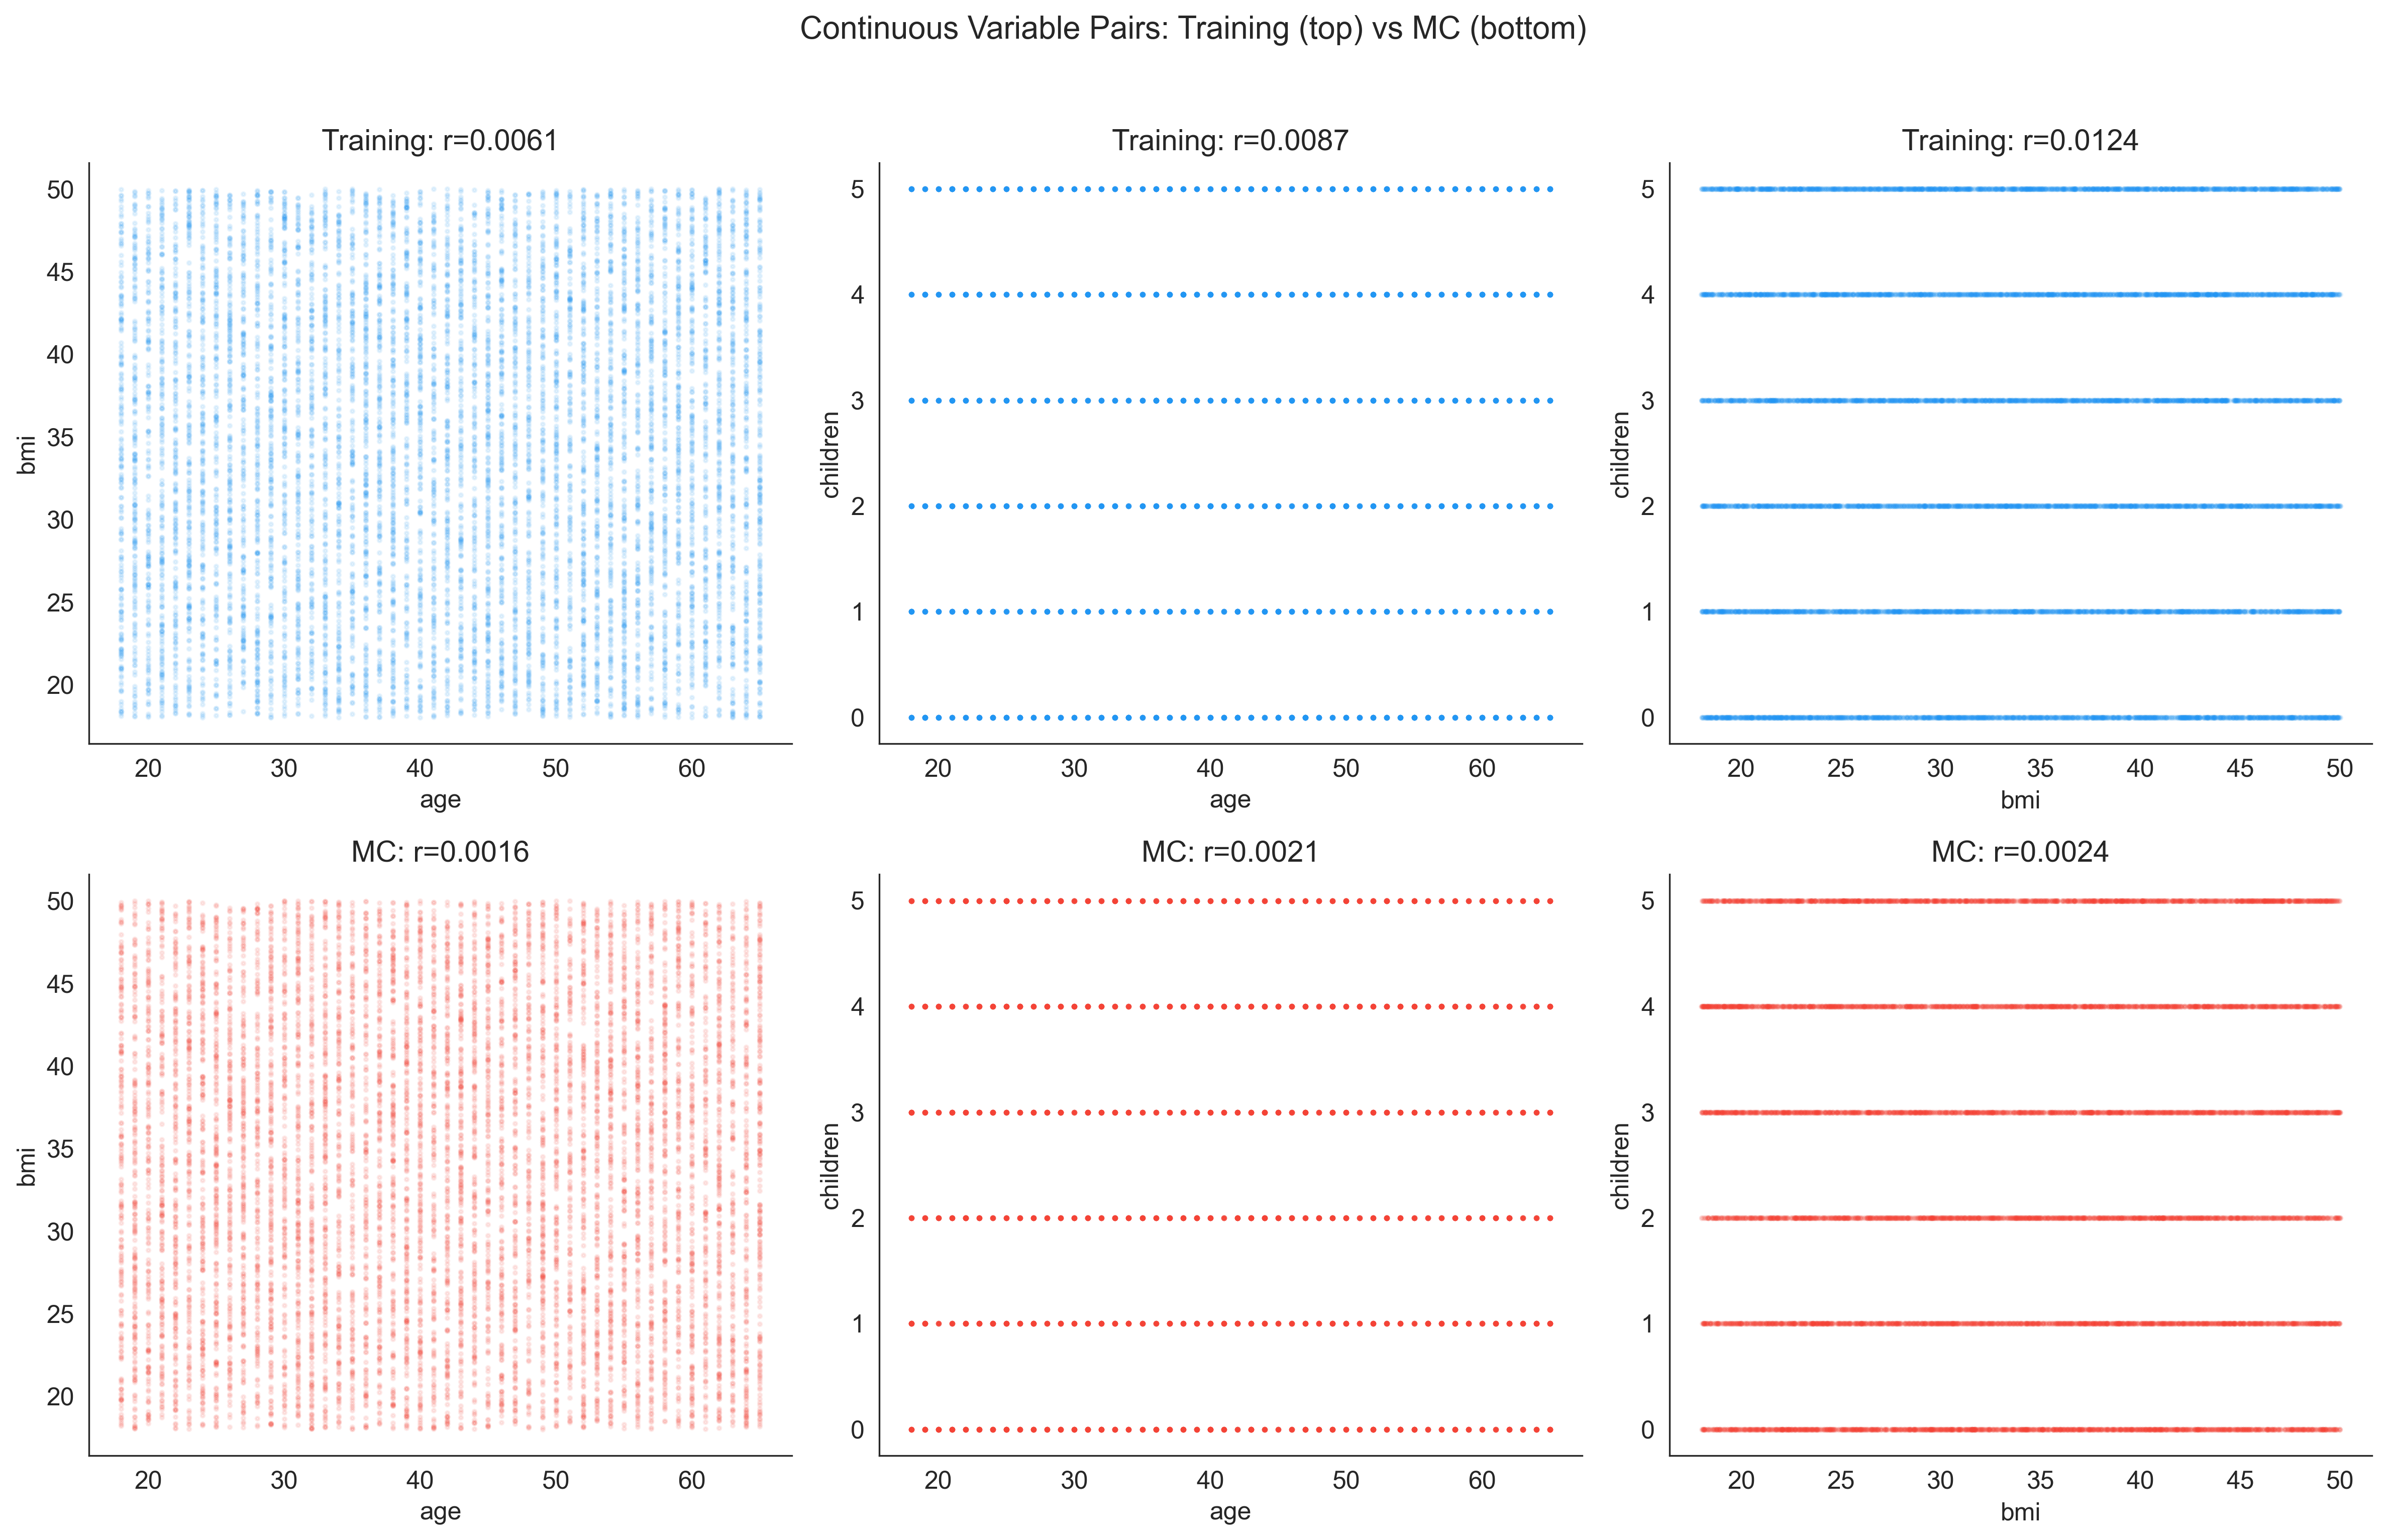
\includegraphics[width=0.95\textwidth]{Thesis/Chapter 4/Figures/fig_mc_joint_continuous_pairs.png}
\caption{Continuous variable pairs: training (top row, blue) versus
Monte Carlo (bottom row, red).}
\label{fig:mc_joint_continuous_pairs_ch4}
\end{figure}

\noindent
Figure~\ref{fig:mc_joint_continuous_pairs_ch4} displays pairwise
scatter plots for the three continuous variables (\texttt{age},
\texttt{bmi}, \texttt{children}).  In the training data, all pairwise
Pearson correlations are negligible ($r = 0.006$, $0.009$, $0.012$).
The Monte Carlo sample shows even weaker correlations ($r = 0.002$,
$0.002$, $0.002$), as expected under independence.  The near-zero
training correlations confirm that the product-marginal simulation does
not discard meaningful continuous dependence.

\begin{figure}[H]
\centering
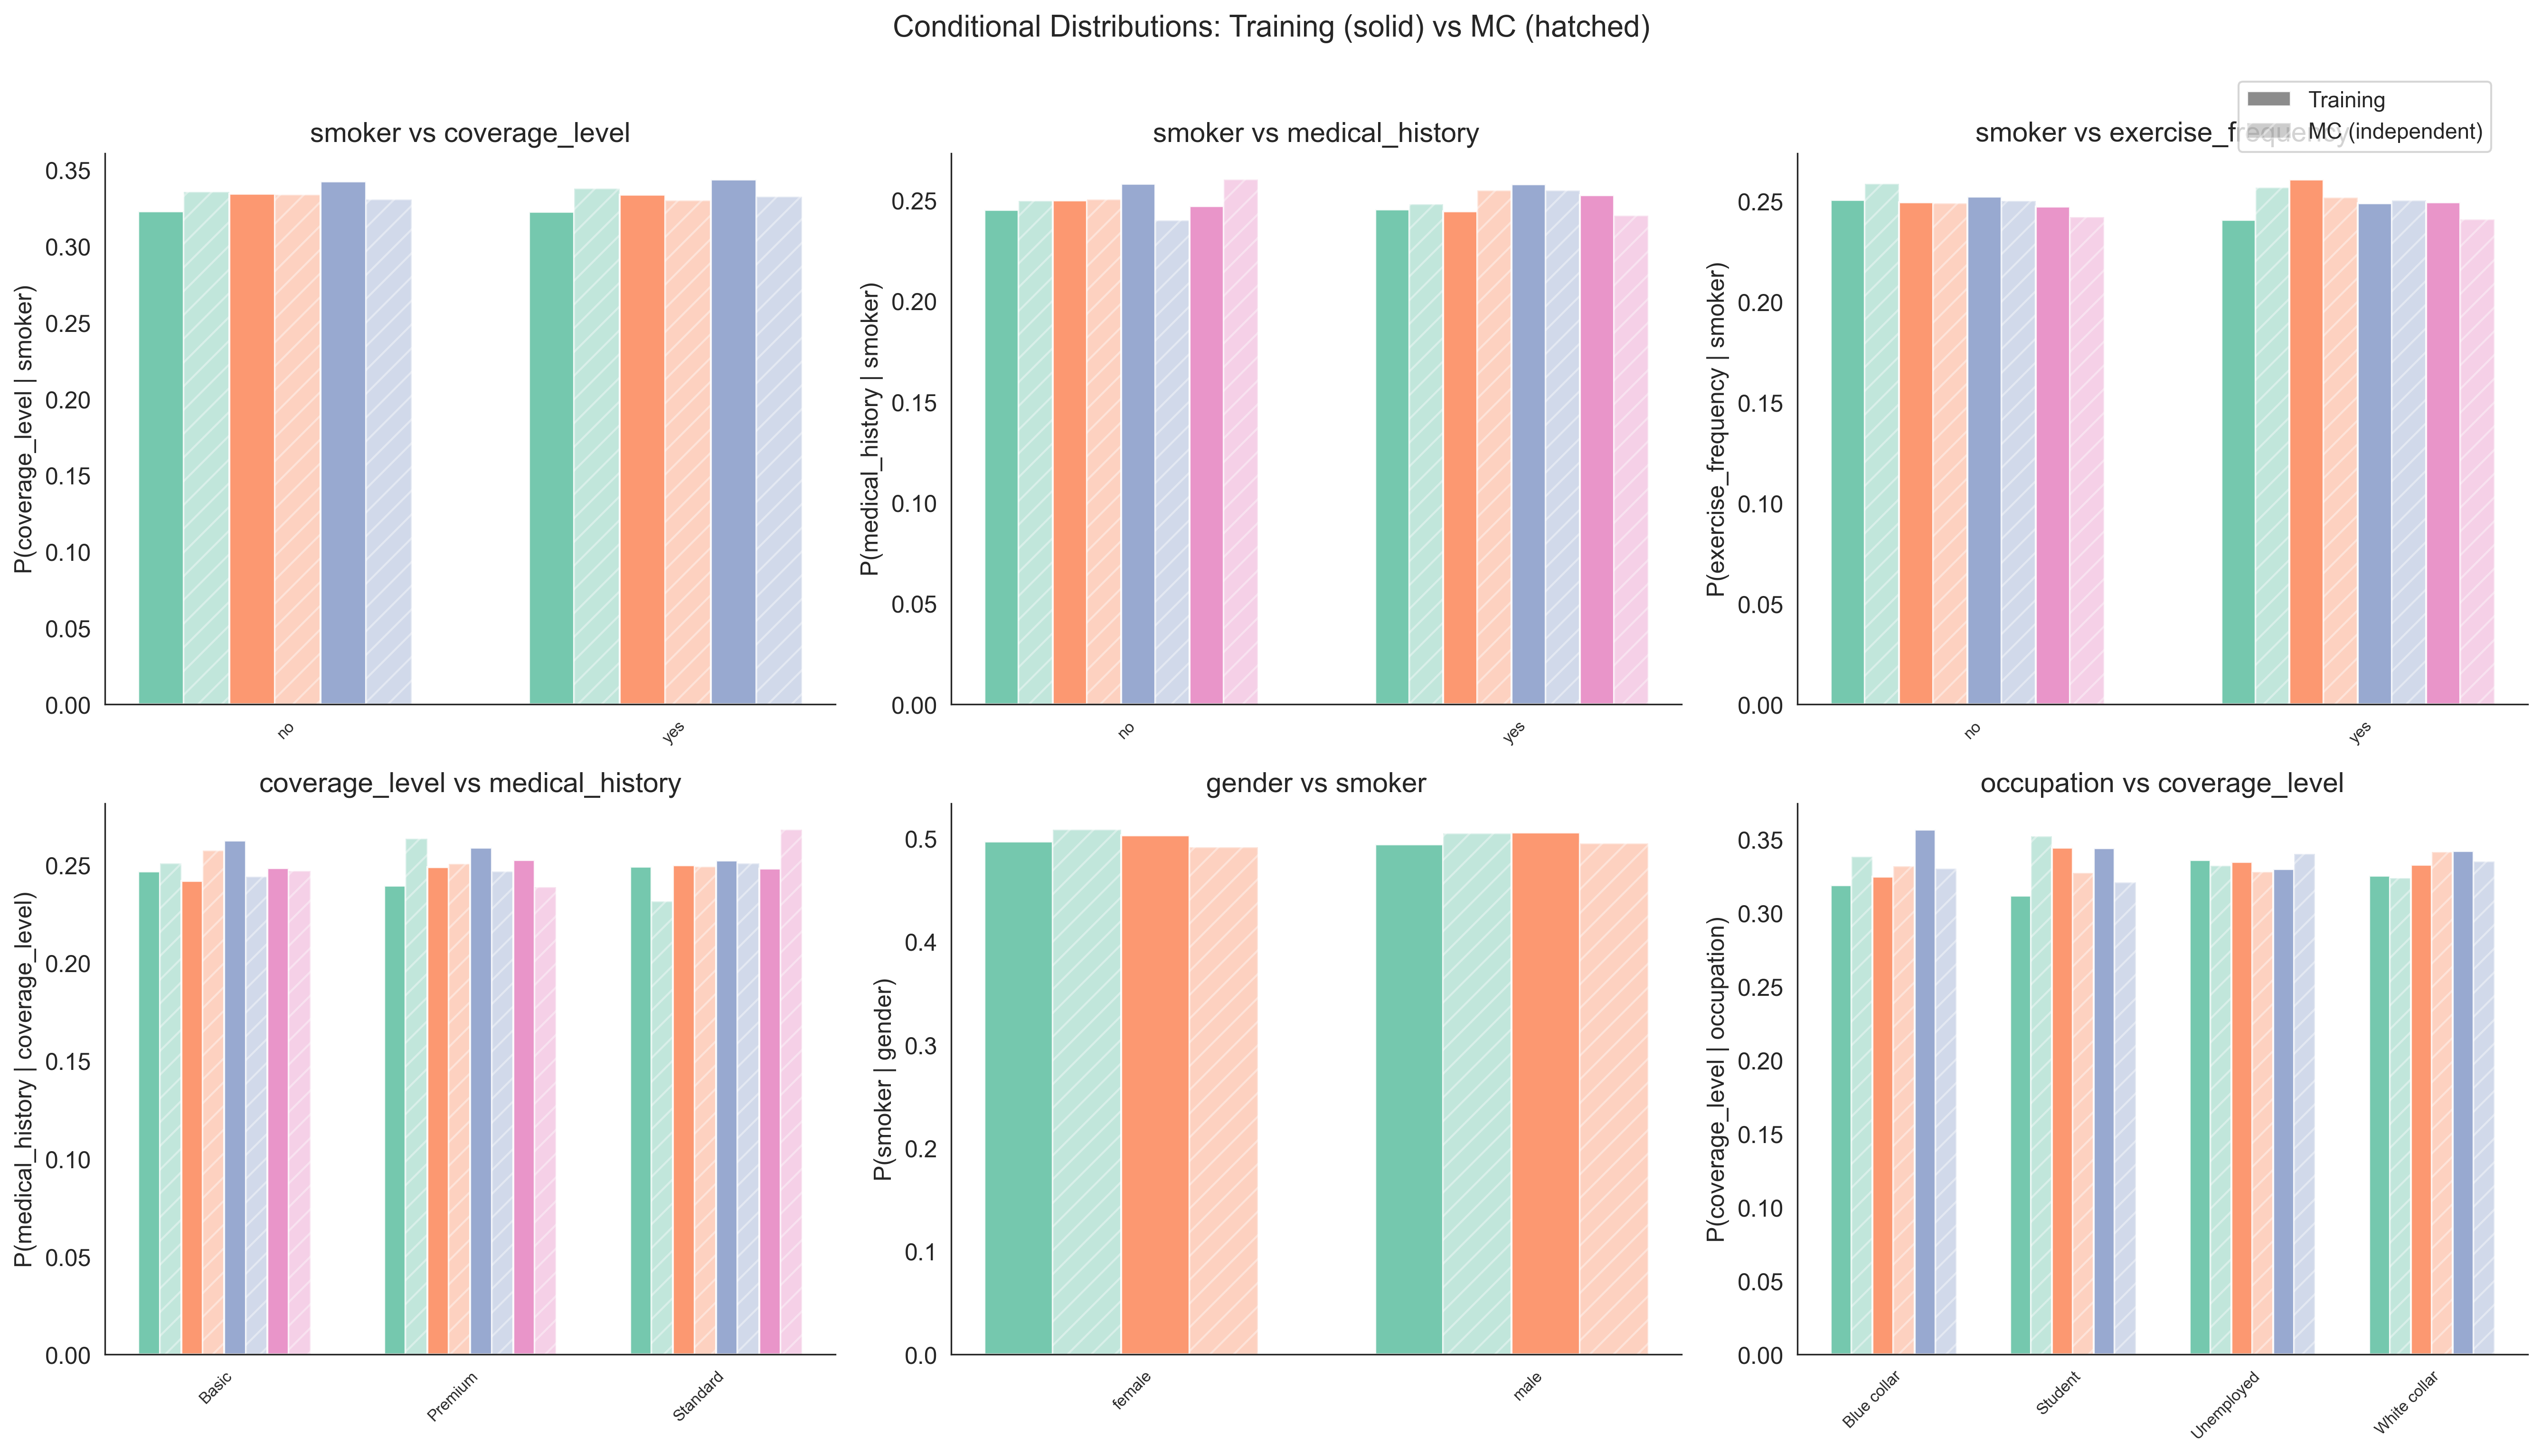
\includegraphics[width=0.95\textwidth]{Thesis/Chapter 4/Figures/fig_mc_joint_crosstabs.png}
\caption{Conditional distributions of selected categorical variable
pairs: training (solid bars) versus Monte Carlo (hatched bars).}
\label{fig:mc_joint_crosstabs_ch4}
\end{figure}

\noindent
Figure~\ref{fig:mc_joint_crosstabs_ch4} compares the conditional
distributions of six key categorical variable pairs.  In each panel,
the conditional proportions are approximately uniform across the
categories of the conditioning variable, both in the training data and
in the Monte Carlo sample.  For instance, the distribution of
\texttt{coverage\_level} given \texttt{smoker} is near-uniform in both
regimes, and the distribution of \texttt{medical\_history} given
\texttt{smoker} is similarly uniform.  These cross-tabulations indicate
that the training-data categoricals are effectively independent of one
another, and the product-marginal simulation preserves this structure.

These bivariate diagnostics complement the correlation-matrix and
Cram\'{e}r's~$V$ comparisons reported in
Section~\ref{sec:mc_input_validation}, which showed that the Pearson
correlation structure and categorical association structure of the
training data are closely reproduced by the parametric Monte Carlo
sample.

\subsubsection*{Higher-order interaction check}

To confirm that the negligible dependence extends beyond pairwise
associations, three-way joint proportions were computed for the four
categorical variables most relevant to the high-cost analysis
(\texttt{smoker}, \texttt{coverage\_level}, \texttt{medical\_history},
\texttt{family\_medical\_history}).

\begin{figure}[H]
\centering
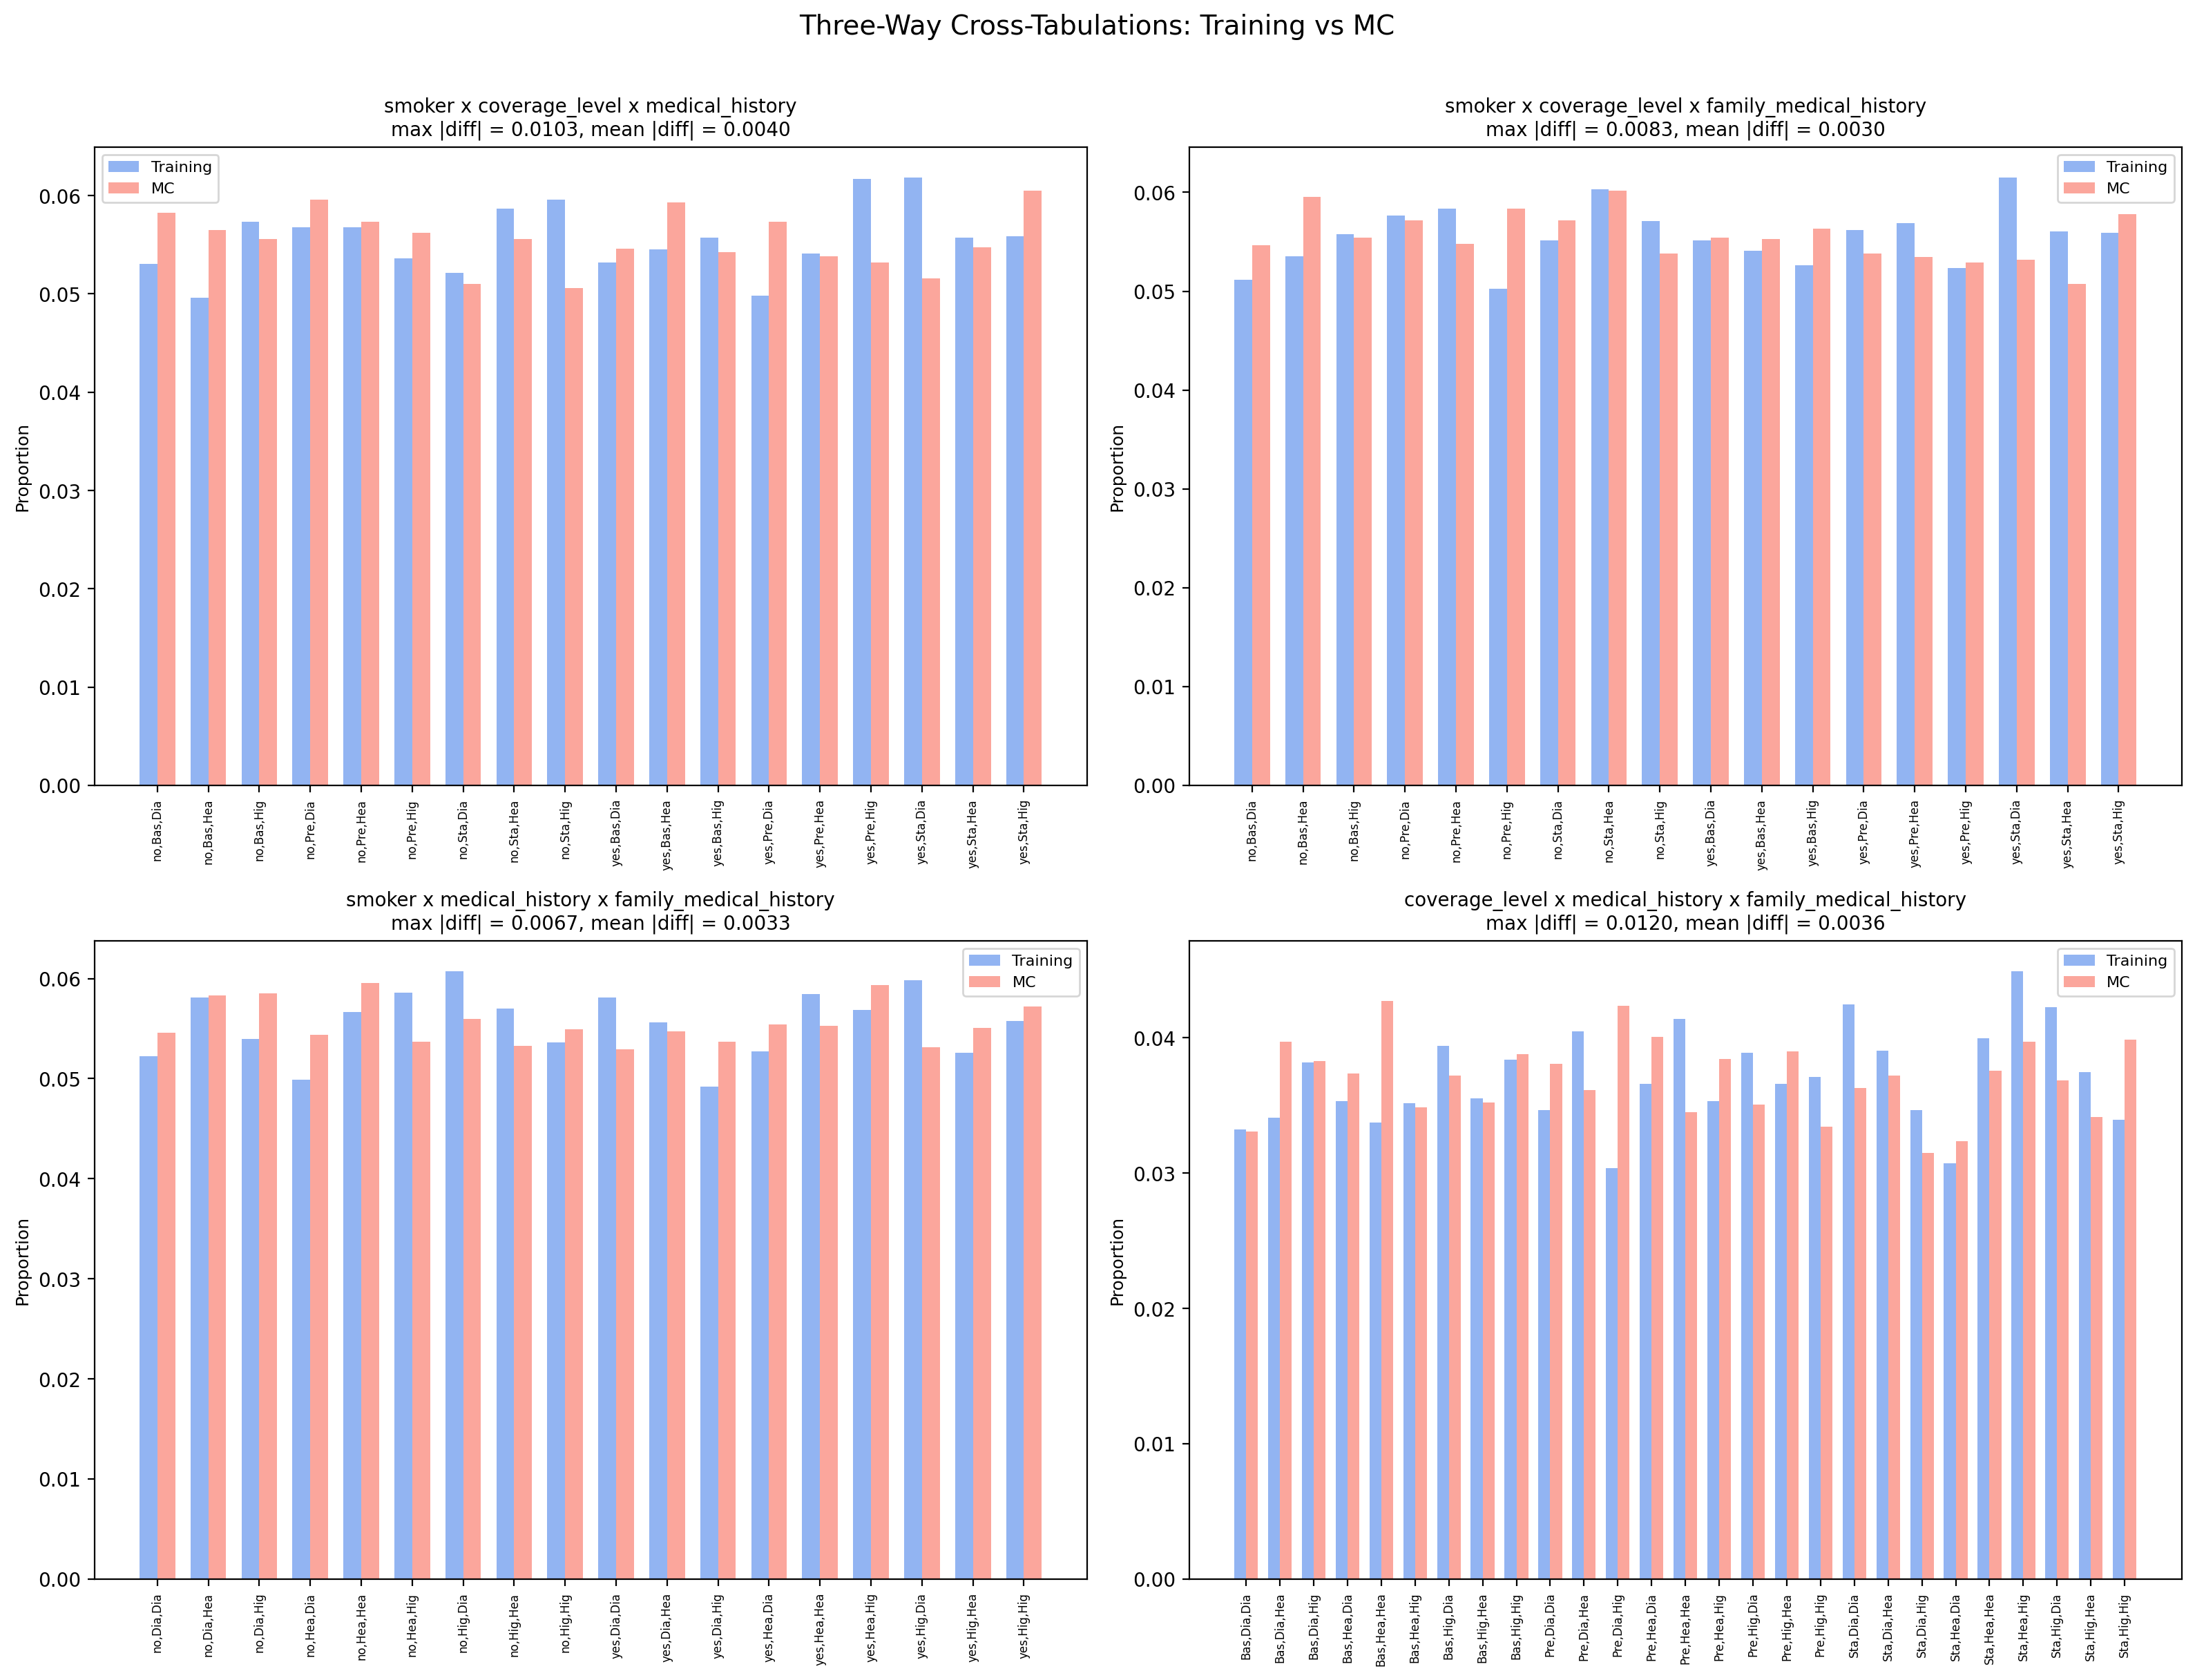
\includegraphics[width=0.95\textwidth]{Thesis/Chapter 4/Figures/fig_threeway_crosstabs.png}
\caption{Three-way cross-tabulations of the four key categorical
variables: training (blue) versus Monte Carlo (red).}
\label{fig:threeway_crosstabs_ch4}
\end{figure}

\noindent
Figure~\ref{fig:threeway_crosstabs_ch4} presents four three-way
cross-tabulations.  Across all triplets, the maximum absolute difference
between the training and Monte Carlo joint proportions is $0.012$
(\texttt{coverage\_level} $\times$ \texttt{medical\_history} $\times$
\texttt{family\_medical\_history}), and the mean absolute differences
are between $0.003$ and $0.004$.  The near-uniform joint proportions in
the training data confirm that higher-order interactions among the
categorical variables are negligible, and the product-marginal
simulation does not discard meaningful multi-way dependence.

\subsubsection*{Multivariate two-sample test}

As a formal test of the overall joint-distribution similarity, the
energy distance between the training and Monte Carlo samples was
computed.

\begin{figure}[H]
\centering
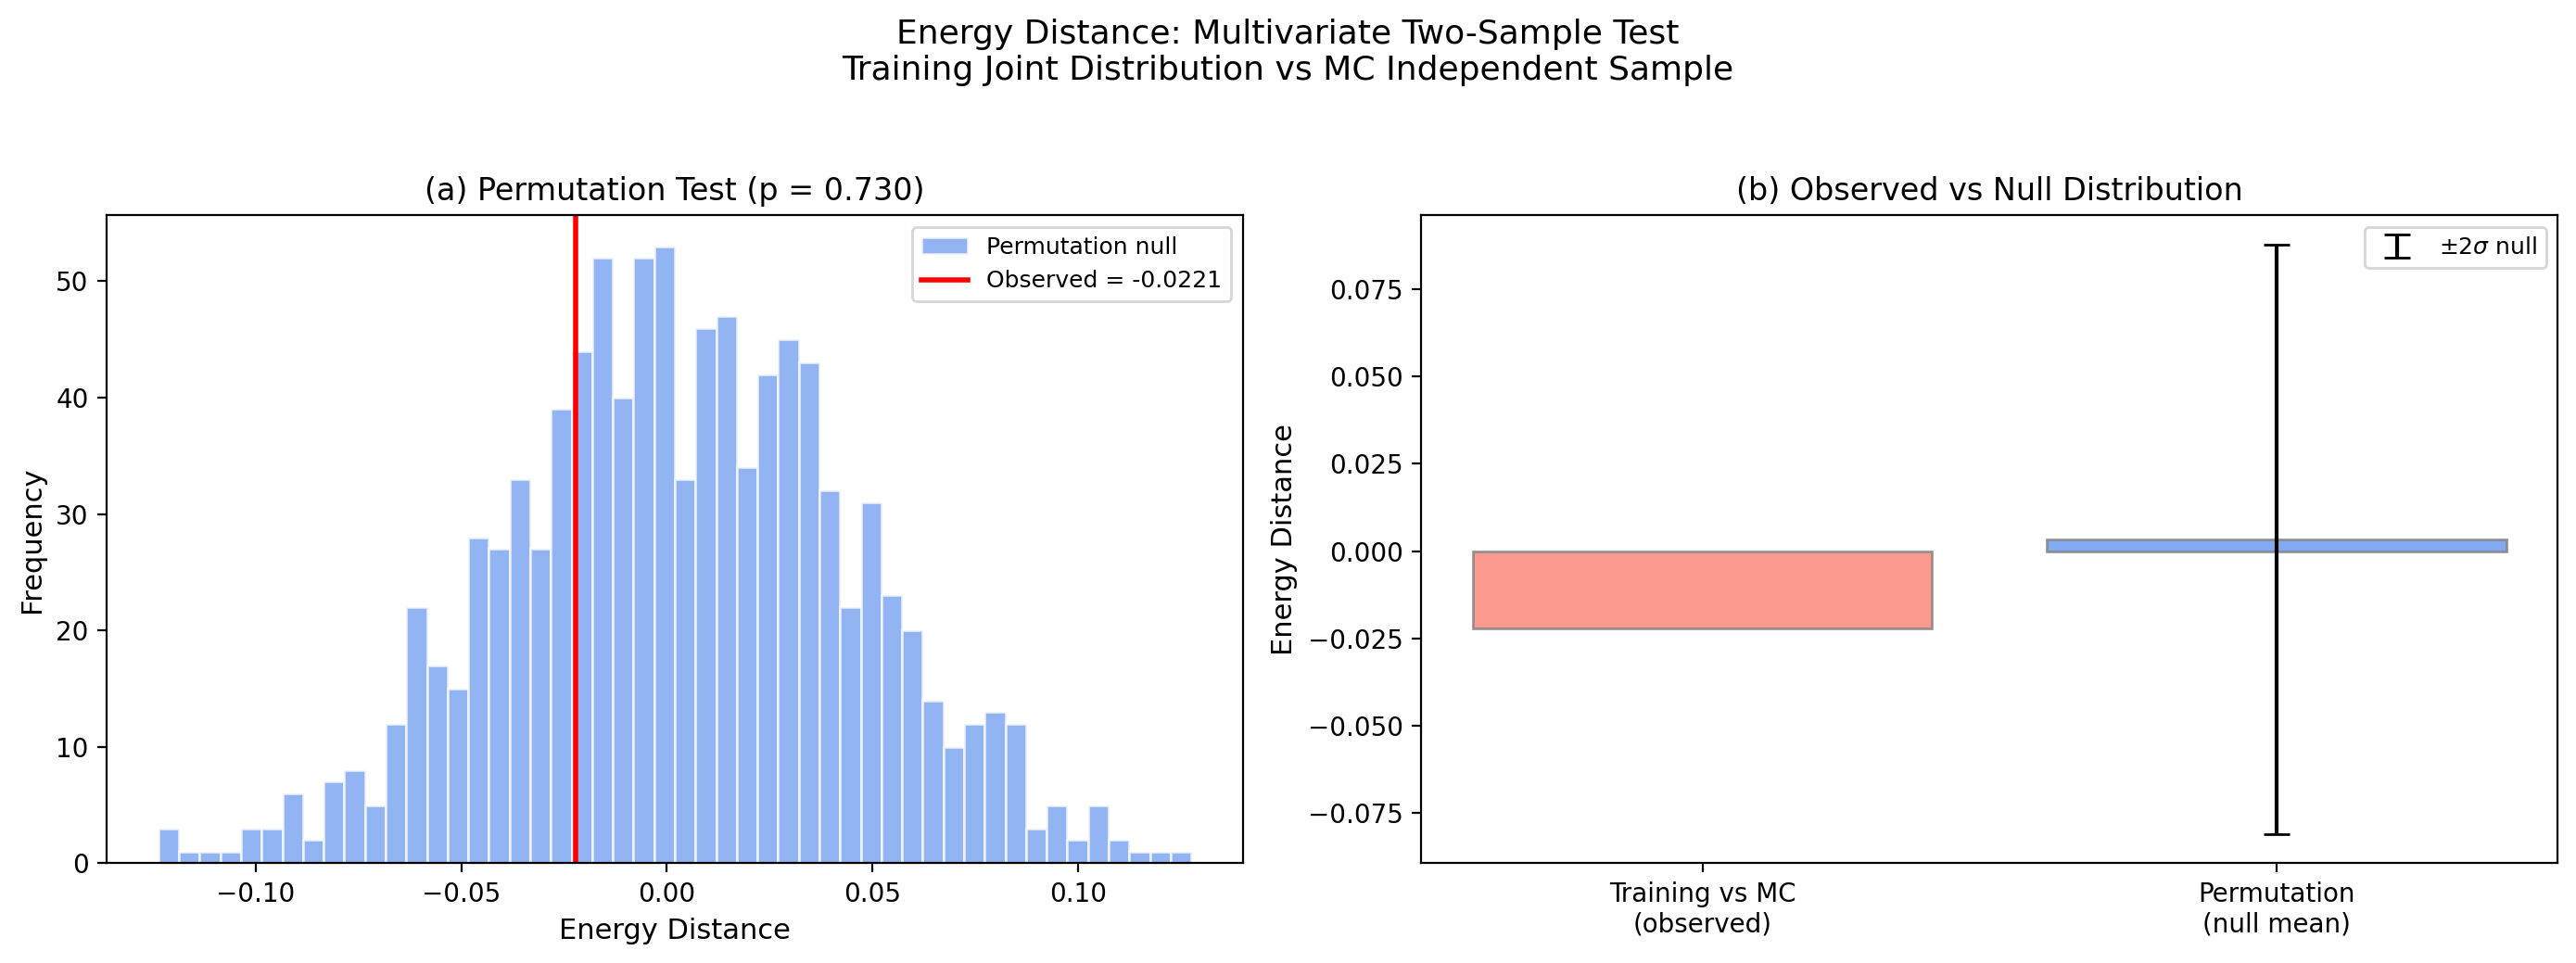
\includegraphics[width=0.95\textwidth]{Thesis/Chapter 4/Figures/fig_energy_distance_test.png}
\caption{Energy distance permutation test: null distribution and observed statistic.}
\label{fig:energy_distance_ch4}
\end{figure}

\noindent
Figure~\ref{fig:energy_distance_ch4} reports the result of a
permutation-based energy distance test with $1\,000$ permutations.  The
observed energy distance is $-0.022$, which falls well within the
permutation null distribution (panel~a).  The permutation $p$-value is
$0.730$, indicating that the observed discrepancy between the training
and Monte Carlo joint distributions is not statistically significant.
The observed energy distance is smaller in magnitude than the null
standard deviation ($0.042$), confirming that the joint distributions
are indistinguishable by this non-parametric criterion.

\subsubsection*{Non-linear manifold overlay}

\begin{figure}[H]
\centering
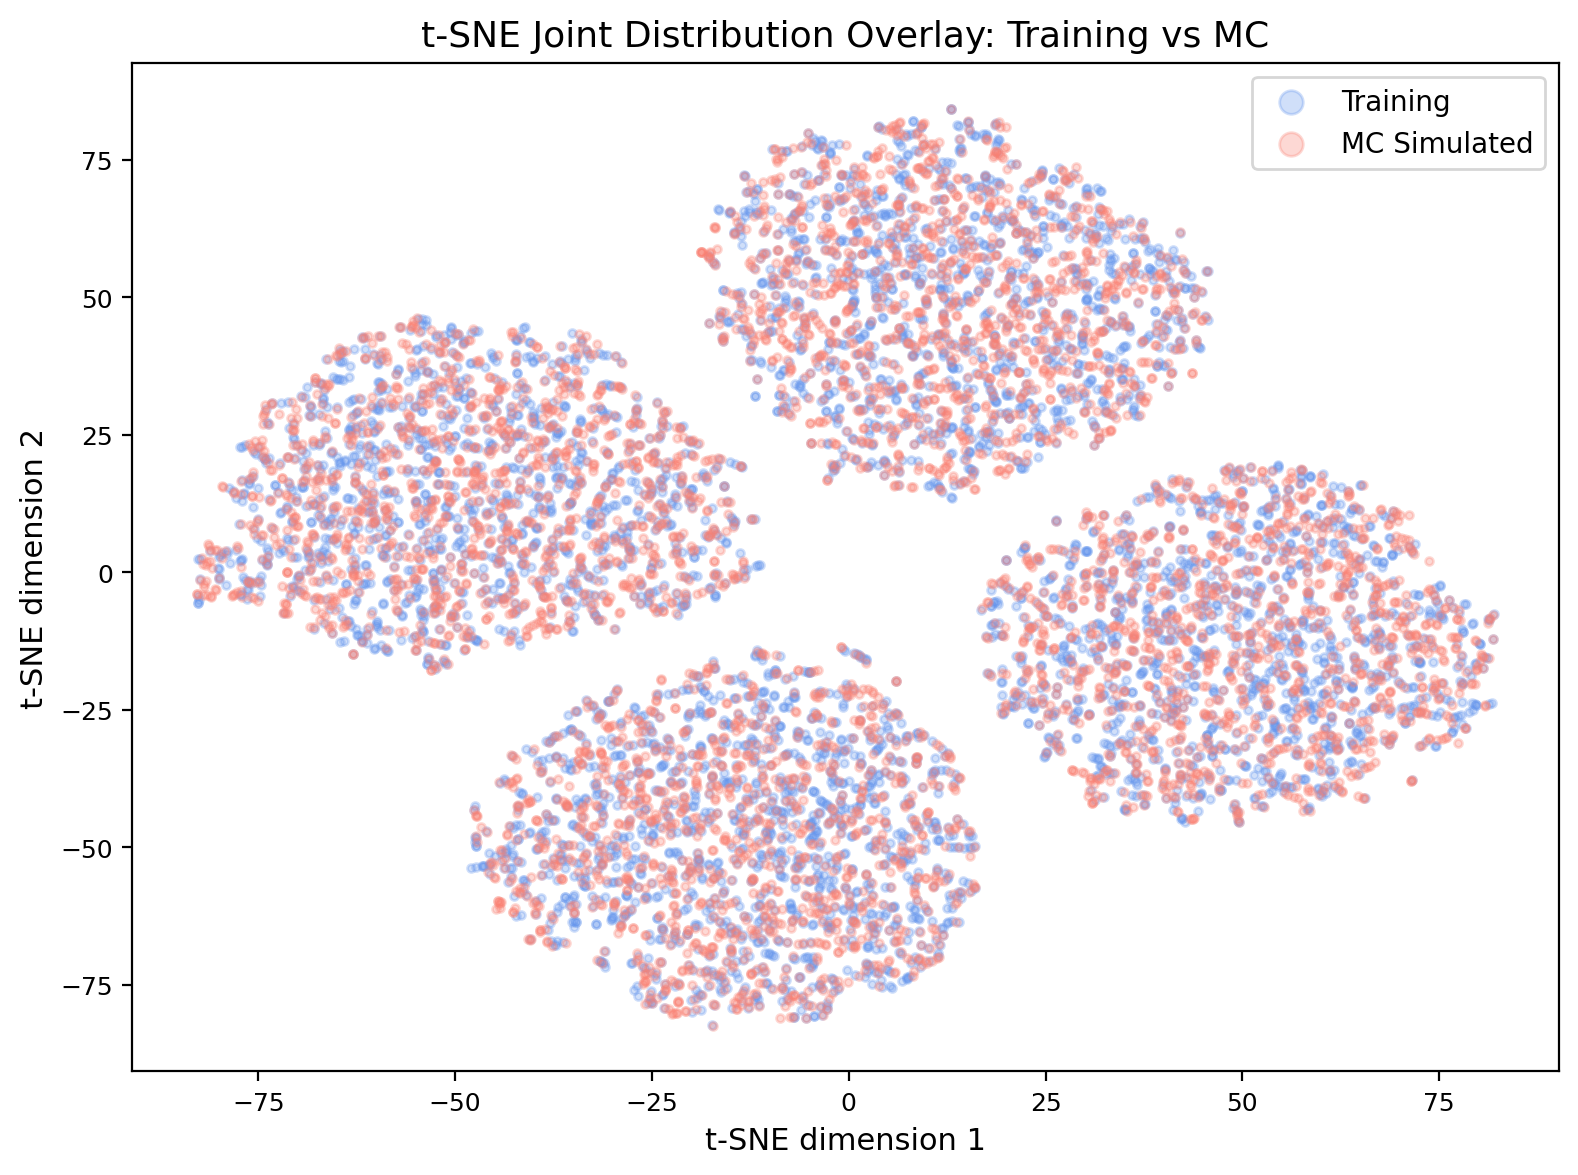
\includegraphics[width=0.70\textwidth]{Thesis/Chapter 4/Figures/fig_tsne_joint_overlay.png}
\caption{t-SNE projection of training versus Monte Carlo joint distributions.}
\label{fig:tsne_joint_overlay_ch4}
\end{figure}

\noindent
Figure~\ref{fig:tsne_joint_overlay_ch4} provides a non-linear
complement to the linear PCA overlay reported in
Section~\ref{sec:mc_input_validation}.  The t-SNE projection maps both
the training and Monte Carlo profiles into two dimensions, preserving
local neighbourhood structure.  The resulting point clouds are
thoroughly intermixed across all identified clusters.  No region of the
manifold is dominated by one sample, confirming that the Monte Carlo
profiles do not occupy novel regions of the feature space that are
unrepresented in the training data.  This result, combined with the PCA
overlay, the energy distance test ($p = 0.730$), and the three-way
cross-tabulations, provides converging evidence that the
product-marginal independence assumption does not materially distort the
joint distributional structure of the training data.

\subsubsection*{Marginal distributions}

\begin{figure}[H]
\centering
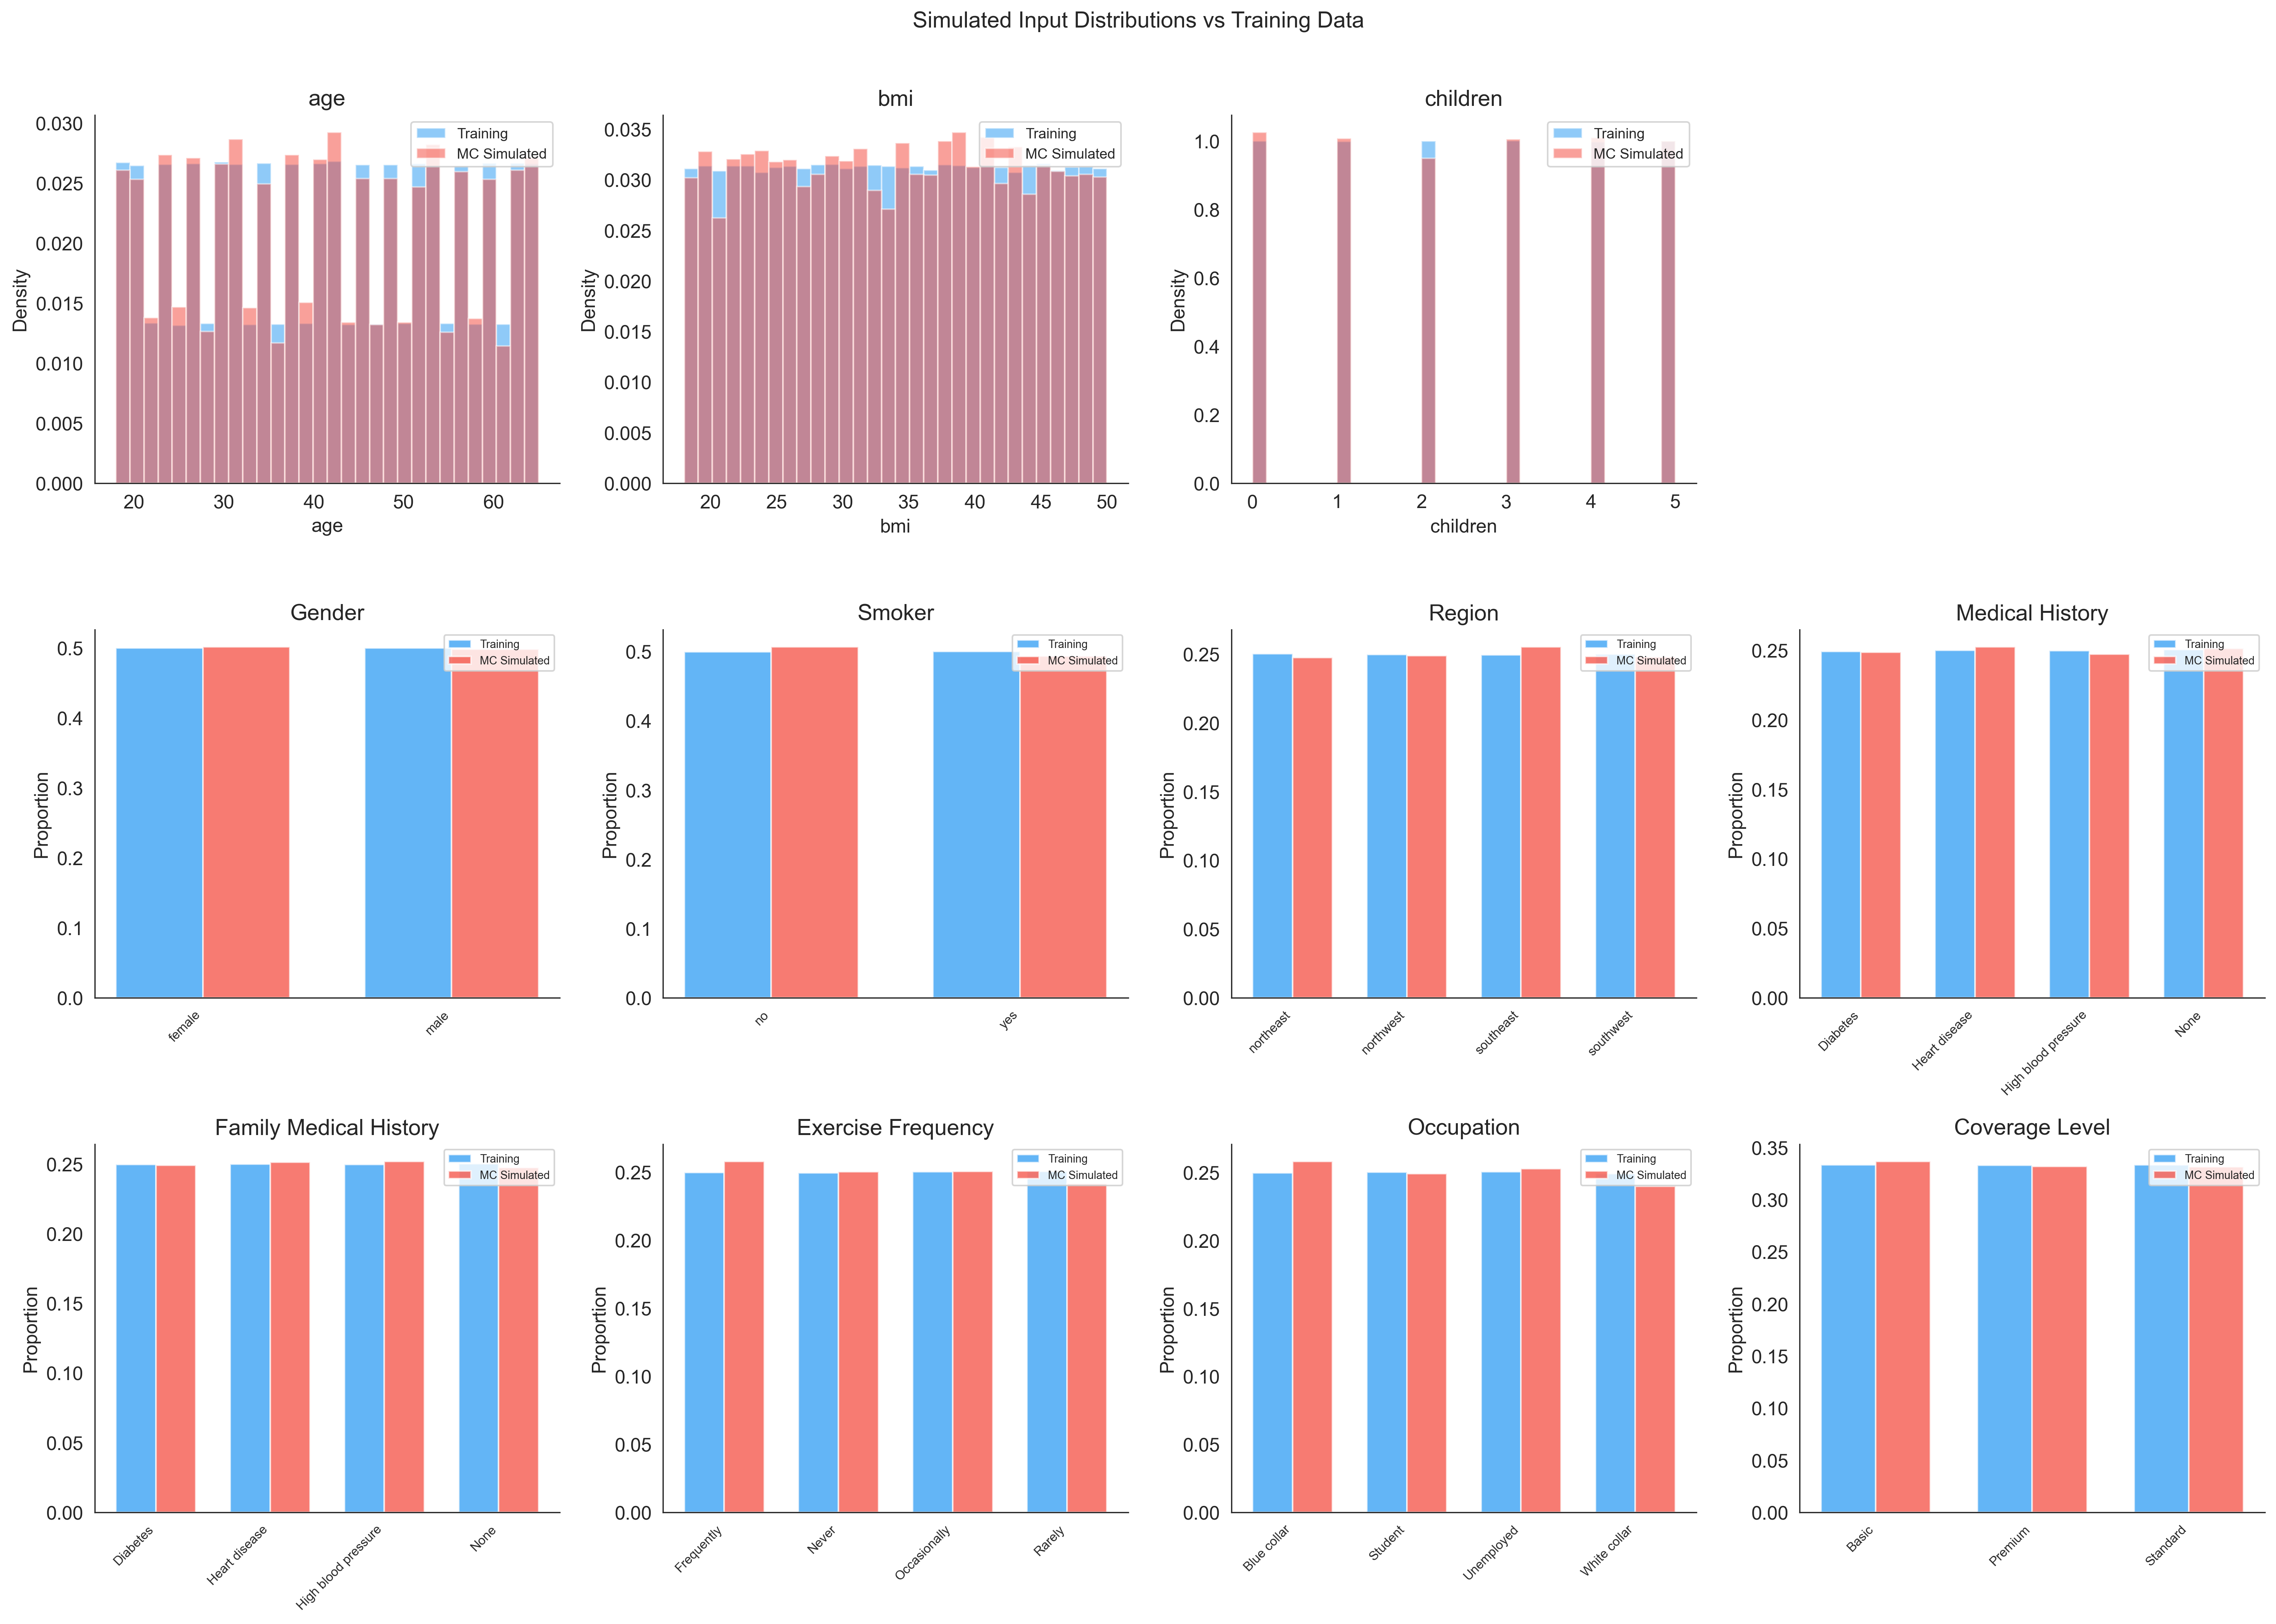
\includegraphics[width=0.95\textwidth]{Thesis/Chapter 4/Figures/fig_mc_input_distributions.png}
\caption{Marginal distributions of all 11 raw predictor variables: training versus Monte Carlo.}
\label{fig:mc_input_distributions_ch4}
\end{figure}

\noindent
Figure~\ref{fig:mc_input_distributions_ch4} confirms that the simulated
marginals closely match the training-data marginals for all 11
variables.  The continuous variables (\texttt{age}, \texttt{bmi}) show
near-uniform histograms in both samples; the discrete count variable
(\texttt{children}) reproduces the approximately equal proportions
across levels 0--5.  For all binary and categorical variables, the
simulated category proportions closely match the training-set
proportions estimated via
equation~\eqref{eq:categorical_probability_estimator_ch3}.  The
parametric simulation therefore faithfully implements the distributional
assumptions stated in Table~\ref{tab:mc_distribution_assumptions_ch3},
at both the joint and marginal levels.

\subsubsection{Model-implied cost distribution}

\begin{figure}[H]
\centering
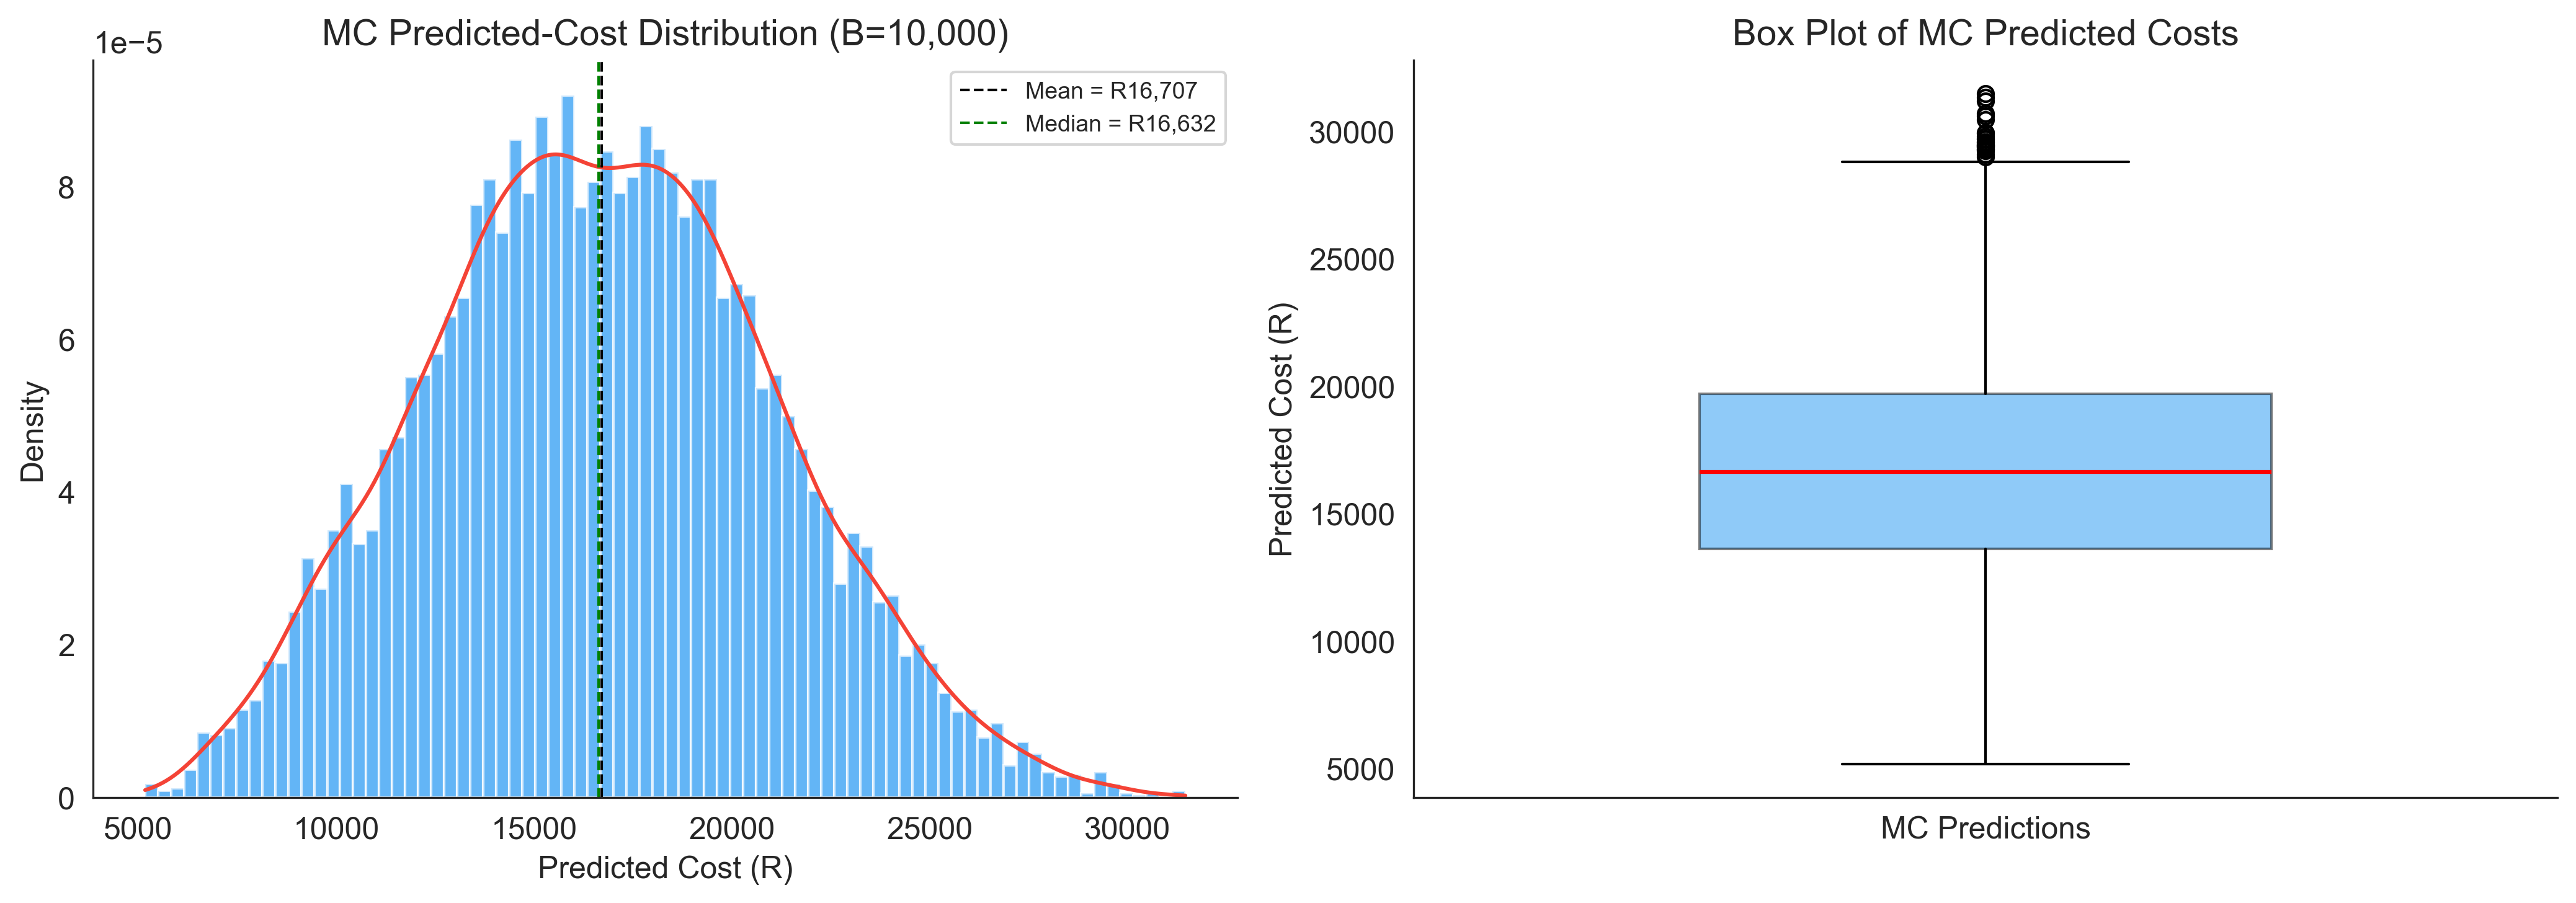
\includegraphics[width=0.95\textwidth]{Thesis/Chapter 4/Figures/fig_mc_predicted_cost_distribution.png}
\caption{Monte Carlo predicted-cost distribution ($B = 10\,000$):
histogram with kernel density overlay (left) and box plot (right).}
\label{fig:mc_predicted_cost_distribution_ch4}
\end{figure}

\noindent
Figure~\ref{fig:mc_predicted_cost_distribution_ch4} displays the
model-implied distribution of predicted insurance costs.
Table~\ref{tab:mc_distribution_summary_ch4} reports the distributional
summary statistics.

\begin{table}[H]
\centering
\caption{Distributional summary of the Monte Carlo predicted costs
($B = 10\,000$).}
\label{tab:mc_distribution_summary_ch4}
\small
\renewcommand{\arraystretch}{1.15}
\begin{tabular}{lr}
\toprule
\textbf{Statistic} & \textbf{Value} \\
\midrule
Mean & R16\,707 \\
Standard deviation & R4\,409 \\
Skewness & $0.128$ \\
Kurtosis & $-0.304$ \\
Minimum & R5\,172 \\
25th percentile & R13\,612 \\
Median & R16\,632 \\
75th percentile & R19\,694 \\
90th percentile & R22\,482 \\
95th percentile & R24\,154 \\
99th percentile & R27\,160 \\
Maximum & R31\,466 \\
\bottomrule
\end{tabular}
\end{table}

\noindent
The distribution is approximately symmetric (skewness $= 0.128$) and
slightly platykurtic (kurtosis $= -0.304$), with a mean of R16\,707 and
a standard deviation of R4\,409. The interquartile range spans
R13\,612 to R19\,694, and the upper tail extends to a maximum predicted
cost of R31\,466. The near-zero skewness and the close agreement
between the mean and median (R16\,707 versus R16\,632) indicate that
the predicted-cost distribution is centred, without heavy-tailed
distortion.

\subsubsection{Convergence diagnostics}

The Monte Carlo standard error and running distributional summaries were
recorded at increasing simulation sizes
$B \in \{1\,000,\; 2\,500,\; 5\,000,\; 10\,000,\; 20\,000\}$
following the convergence monitoring procedure in
Section~\ref{sec:mc_simulation_design}.

\begin{figure}[H]
\centering
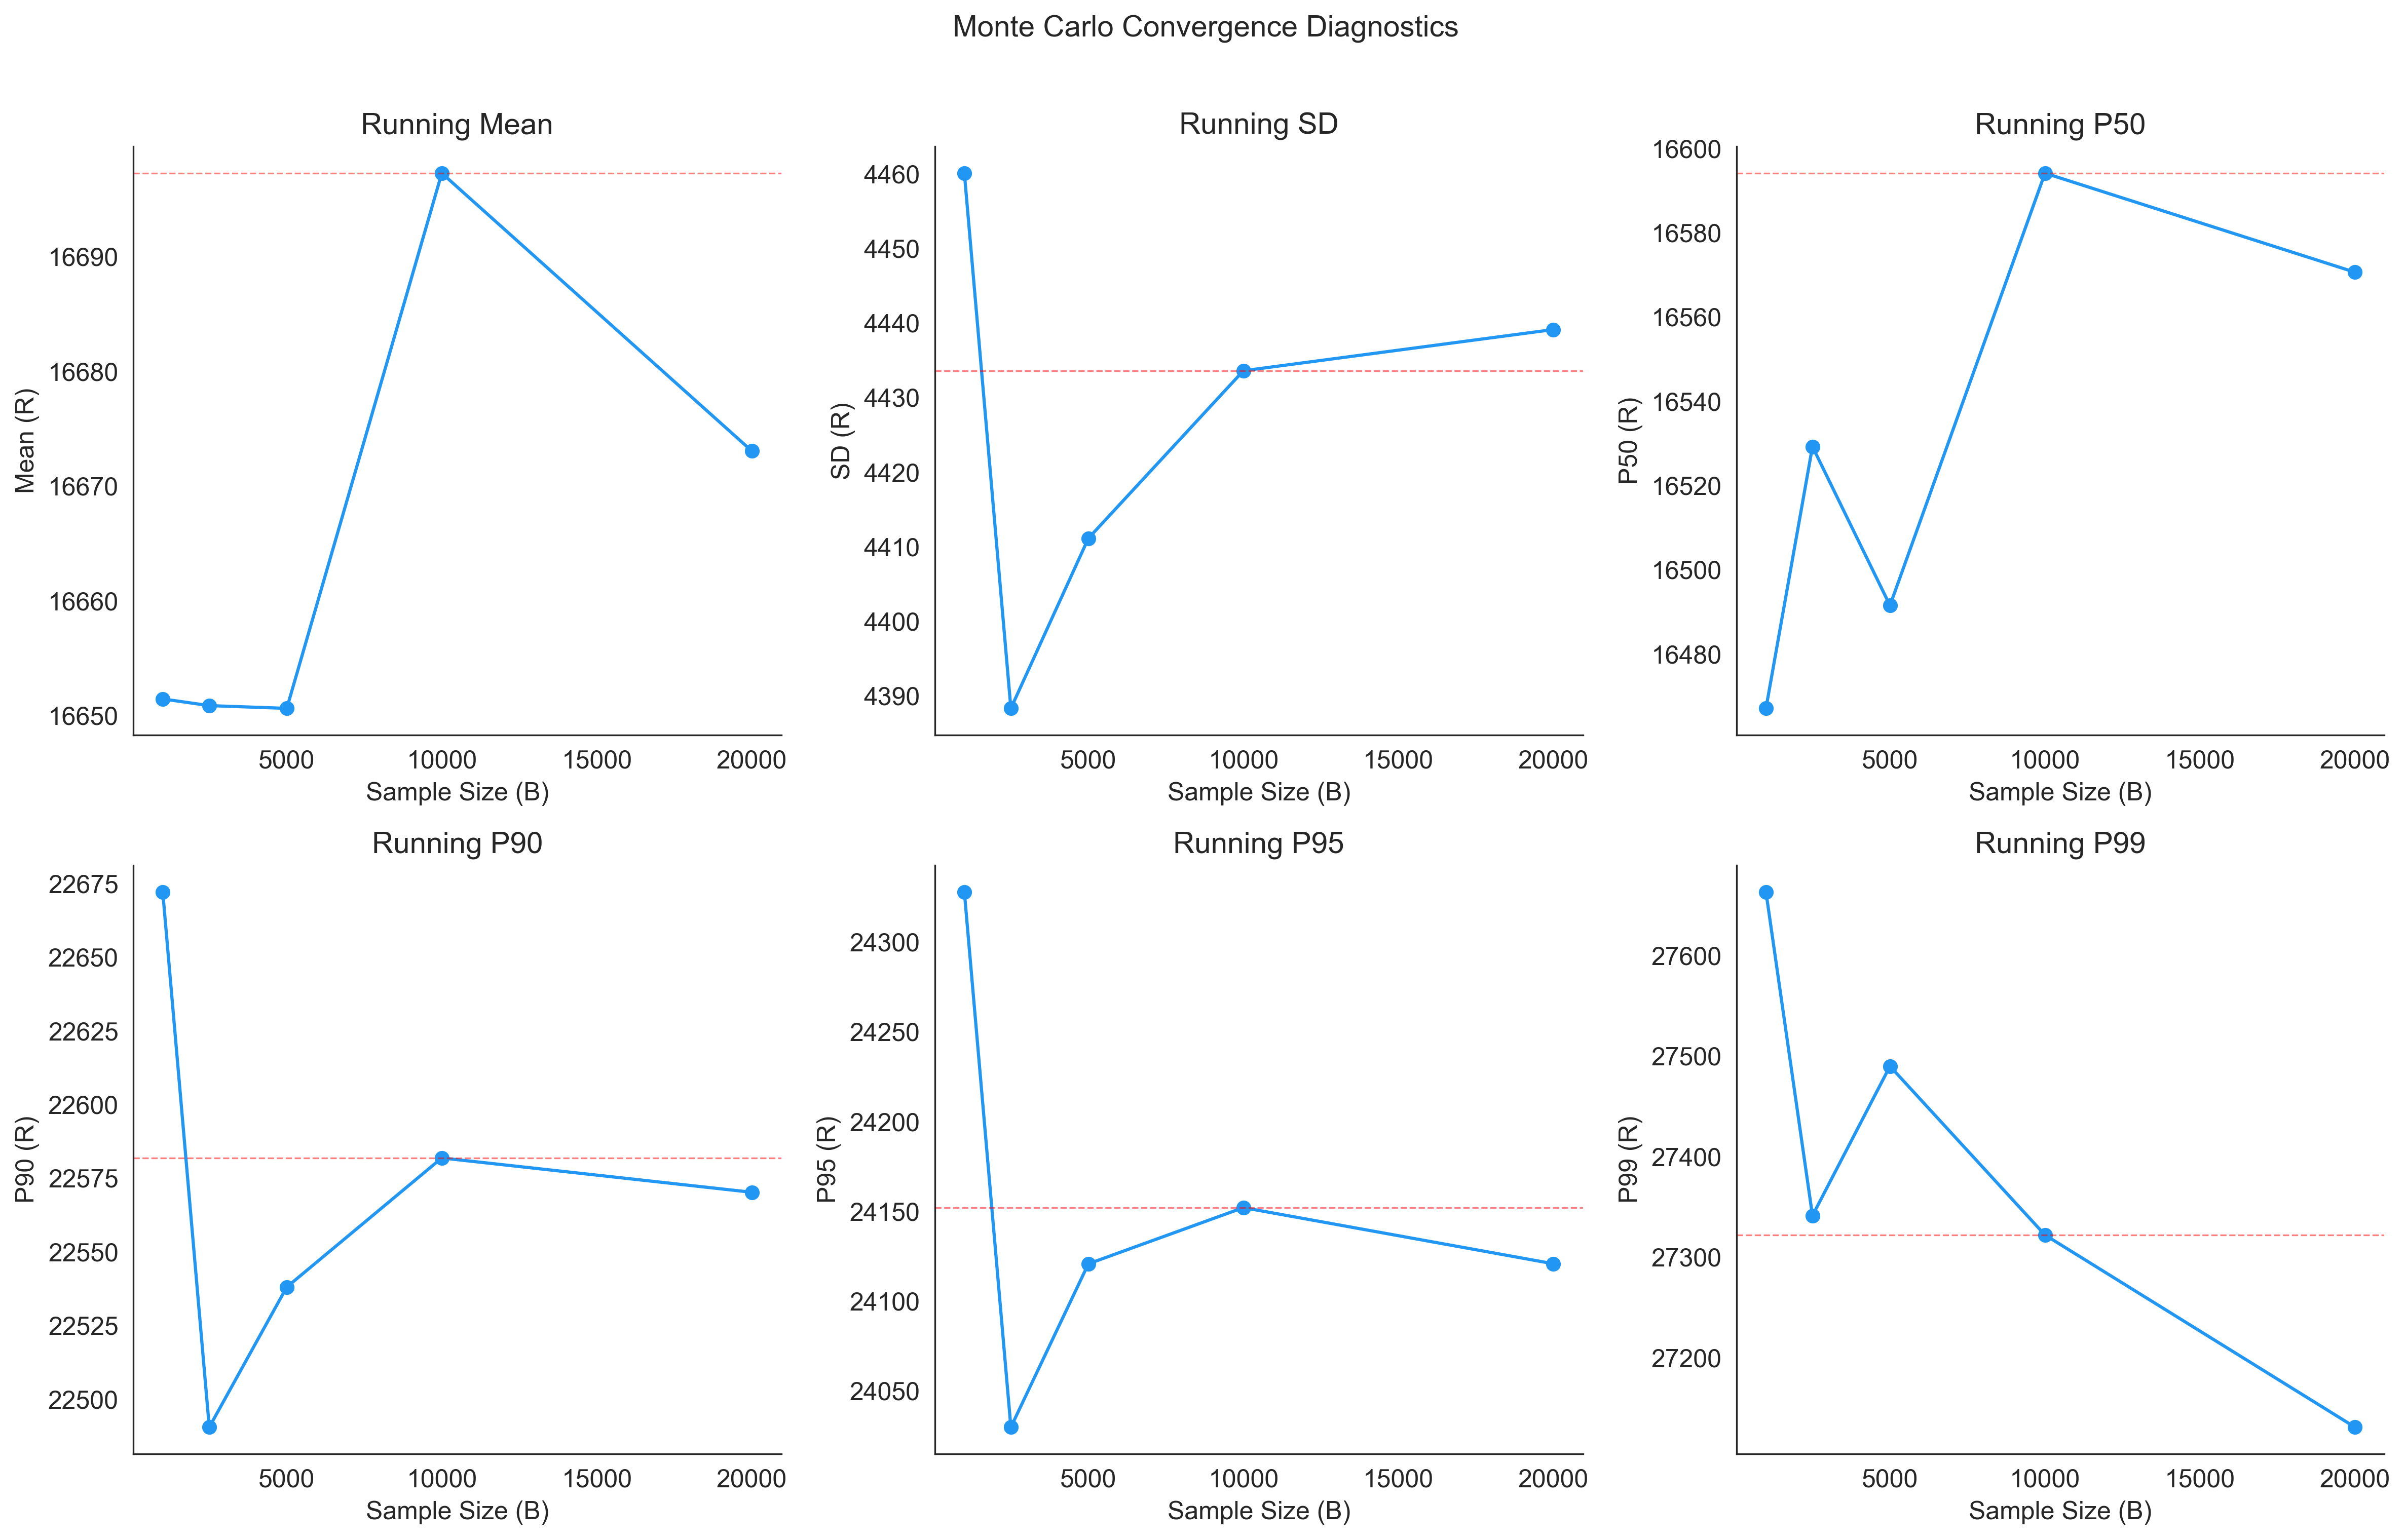
\includegraphics[width=0.95\textwidth]{Thesis/Chapter 4/Figures/fig_mc_convergence.png}
\caption{Monte Carlo convergence diagnostics by simulation size $B$.}
\label{fig:mc_convergence_ch4}
\end{figure}

\noindent
Figure~\ref{fig:mc_convergence_ch4} shows that the running mean
stabilises within a narrow band (R16\,651 to R16\,697) across all
simulation sizes. The running standard deviation converges from R4\,460
at $B = 1\,000$ to R4\,439 at $B = 20\,000$. The median and upper-tail
quantiles exhibit similar stability, with the 95th percentile ranging
from R24\,030 to R24\,328 across all sizes.
Table~\ref{tab:mc_convergence_ch4} reports the \gls{mcse} at each
simulation size.

\begin{table}[H]
\centering
\caption{Monte Carlo convergence: running summaries and MCSE by
simulation size.}
\label{tab:mc_convergence_ch4}
\small
\renewcommand{\arraystretch}{1.15}
\begin{tabular}{rrrrrrrr}
\toprule
$B$ & Mean & SD & Median & P90 & P95 & P99 & MCSE \\
\midrule
1\,000 & 16\,651 & 4\,460 & 16\,467 & 22\,672 & 24\,328 & 27\,663 & 141.0 \\
2\,500 & 16\,651 & 4\,388 & 16\,529 & 22\,490 & 24\,030 & 27\,341 & 87.8 \\
5\,000 & 16\,651 & 4\,411 & 16\,492 & 22\,538 & 24\,121 & 27\,490 & 62.4 \\
10\,000 & 16\,697 & 4\,434 & 16\,594 & 22\,582 & 24\,152 & 27\,322 & 44.3 \\
20\,000 & 16\,673 & 4\,439 & 16\,571 & 22\,570 & 24\,121 & 27\,131 & 31.4 \\
\bottomrule
\end{tabular}
\end{table}

\noindent
The \gls{mcse} decreases from R141 at $B = 1\,000$ to R44.3 at
$B = 10\,000$, representing $0.27\%$ of the mean predicted cost. At the
selected simulation size of $B = 10\,000$, the running summaries have
stabilised and the simulation precision is adequate for the subsequent
distributional and attribution analyses.

\subsubsection{Comparison with observed training charges}

\begin{figure}[H]
\centering
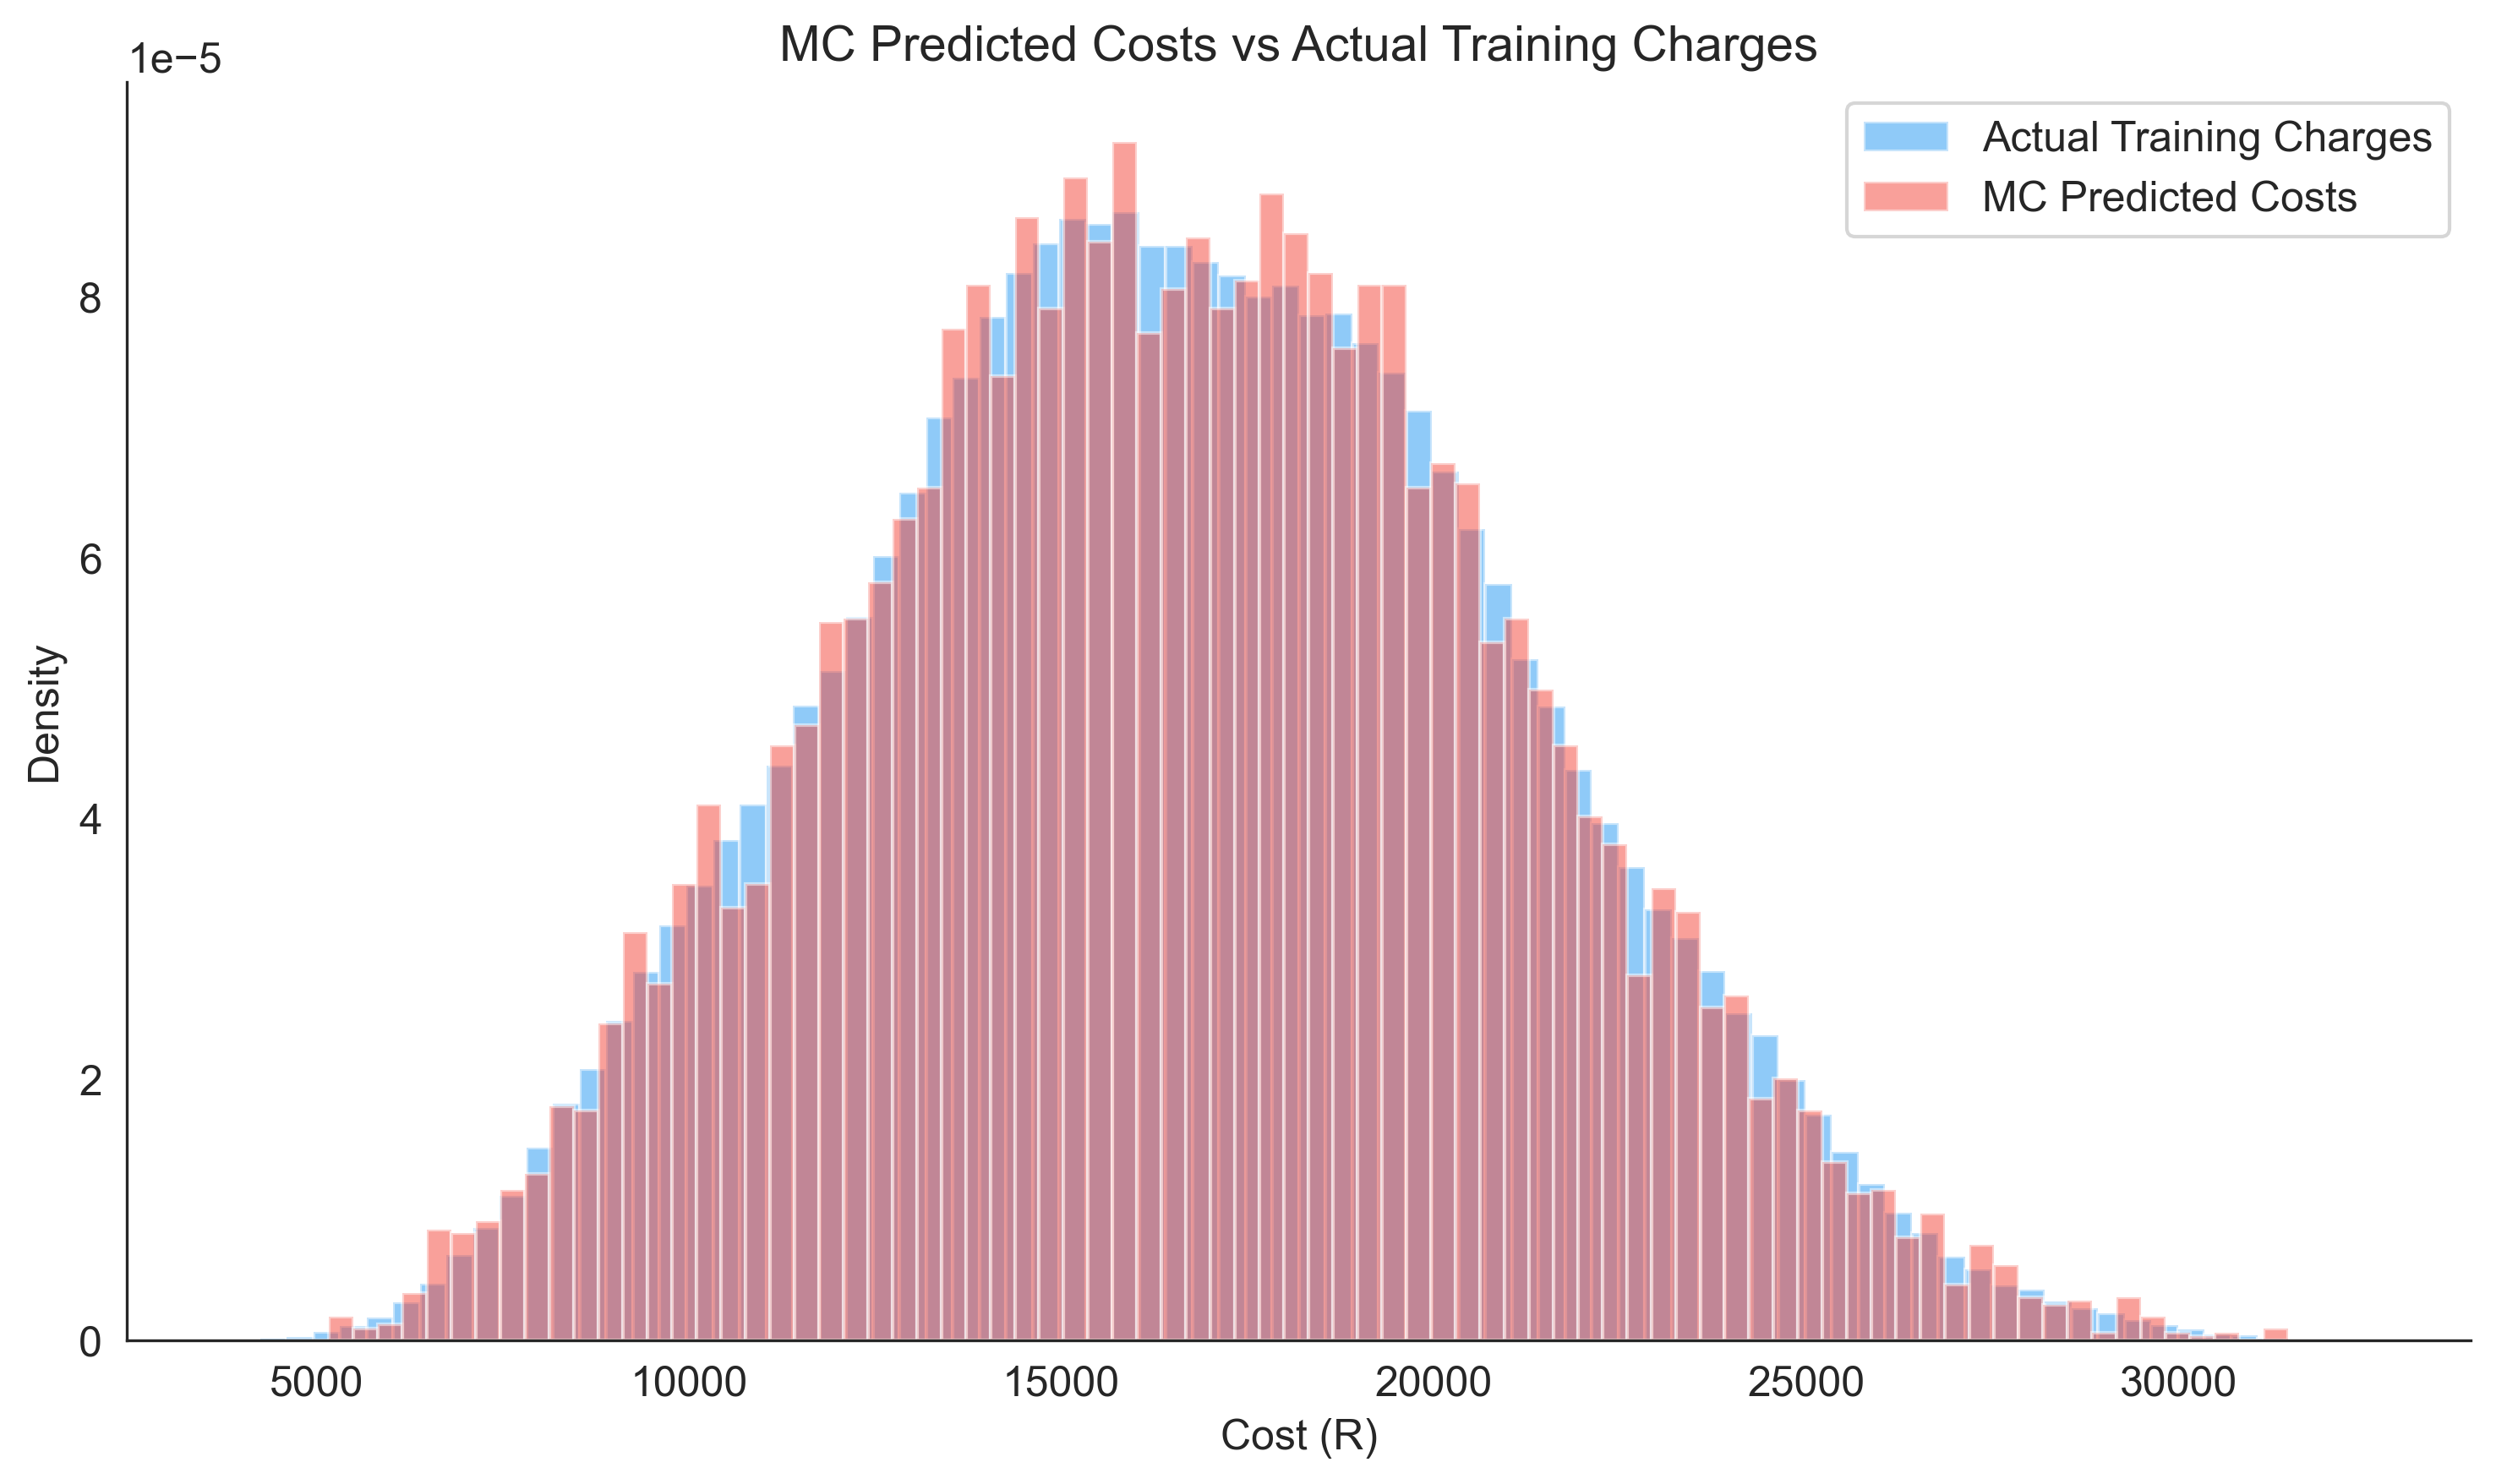
\includegraphics[width=0.80\textwidth]{Thesis/Chapter 4/Figures/fig_mc_predicted_vs_actual.png}
\caption{Overlay of the Monte Carlo predicted-cost distribution (red)
and the observed training-set charge distribution (blue).}
\label{fig:mc_predicted_vs_actual_ch4}
\end{figure}

\noindent
Figure~\ref{fig:mc_predicted_vs_actual_ch4} overlays the Monte Carlo
predicted-cost histogram with the observed training-set charge
distribution. The two distributions share similar location, spread and
shape: both are unimodal, roughly symmetric, and span the range from
approximately R5\,000 to R32\,000. The close agreement confirms that
the fitted \gls{dnn}, when evaluated on profiles drawn from the
parametric input distribution, produces a predicted-cost landscape that
is consistent with the distributional characteristics of the observed
training data. Minor differences in the tails reflect the smoothing
behaviour of the regression model and the slight mismatch between the
product-marginal simulation law and the empirical joint distribution.


% =============================================================
\subsection{Residual-Augmented Monte Carlo Sensitivity}
\label{sec:residual_augmented_results}

The residual-augmented sensitivity analysis
(Section~\ref{sec:residual_augmented_mc}) was applied to the
$B = 10\,000$ base Monte Carlo predictions.  Centred fitted residuals
were drawn from the empirical residual distribution
$\widehat{F}_{\varepsilon}$
(equation~\eqref{eq:residual_draw_ch3}), and a fixed perturbation band
of $\pm 0.5\,\widehat{\sigma}_{\varepsilon}$ was computed following
equation~\eqref{eq:fixed_residual_perturbation_ch3}.

\begin{figure}[H]
\centering
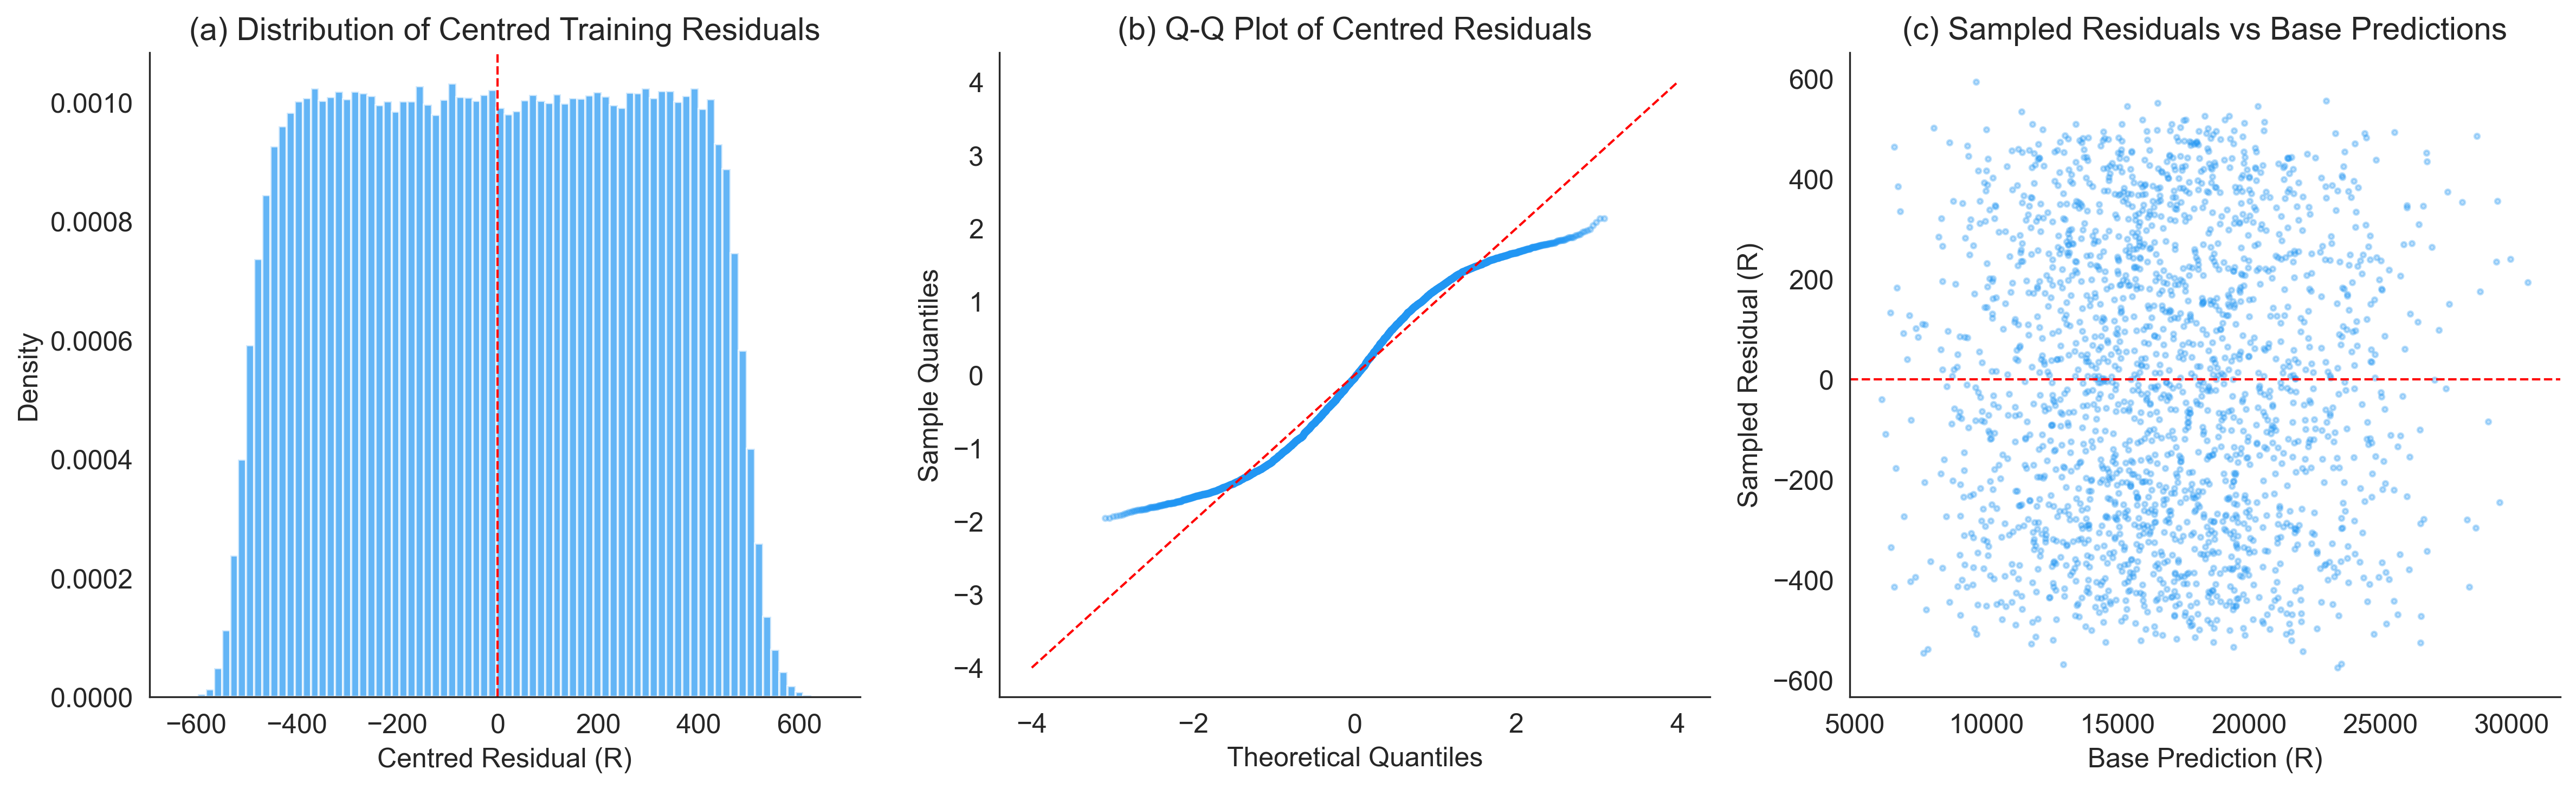
\includegraphics[width=0.95\textwidth]{Thesis/Chapter 4/Figures/fig_mc_residual_diagnostics.png}
\caption{Centred training residual diagnostics for the augmented simulation.}
\label{fig:mc_residual_diagnostics_ch4}
\end{figure}

\noindent
Figure~\ref{fig:mc_residual_diagnostics_ch4} characterises the centred
training residuals from which the augmented draws are sampled.  The
histogram in panel~(a) is symmetric and bell-shaped, confirming that the
residual distribution is well-centred and does not contain systematic
bias.  The Q-Q plot in panel~(b) shows slight tail compression relative
to a Gaussian reference, consistent with the mild platykurtic behaviour
noted in the model diagnostics of
Section~\ref{sec:model_validation_diagnostics}.  Panel~(c) plots the
sampled residuals against the base predictions: the scatter is random
and centred at zero across the full prediction range (R5\,000 to
R30\,000), indicating that the residual magnitude does not depend on the
predicted cost level.  These properties confirm that the empirical
residual distribution is suitable for the perturbation analysis.

\begin{figure}[H]
\centering
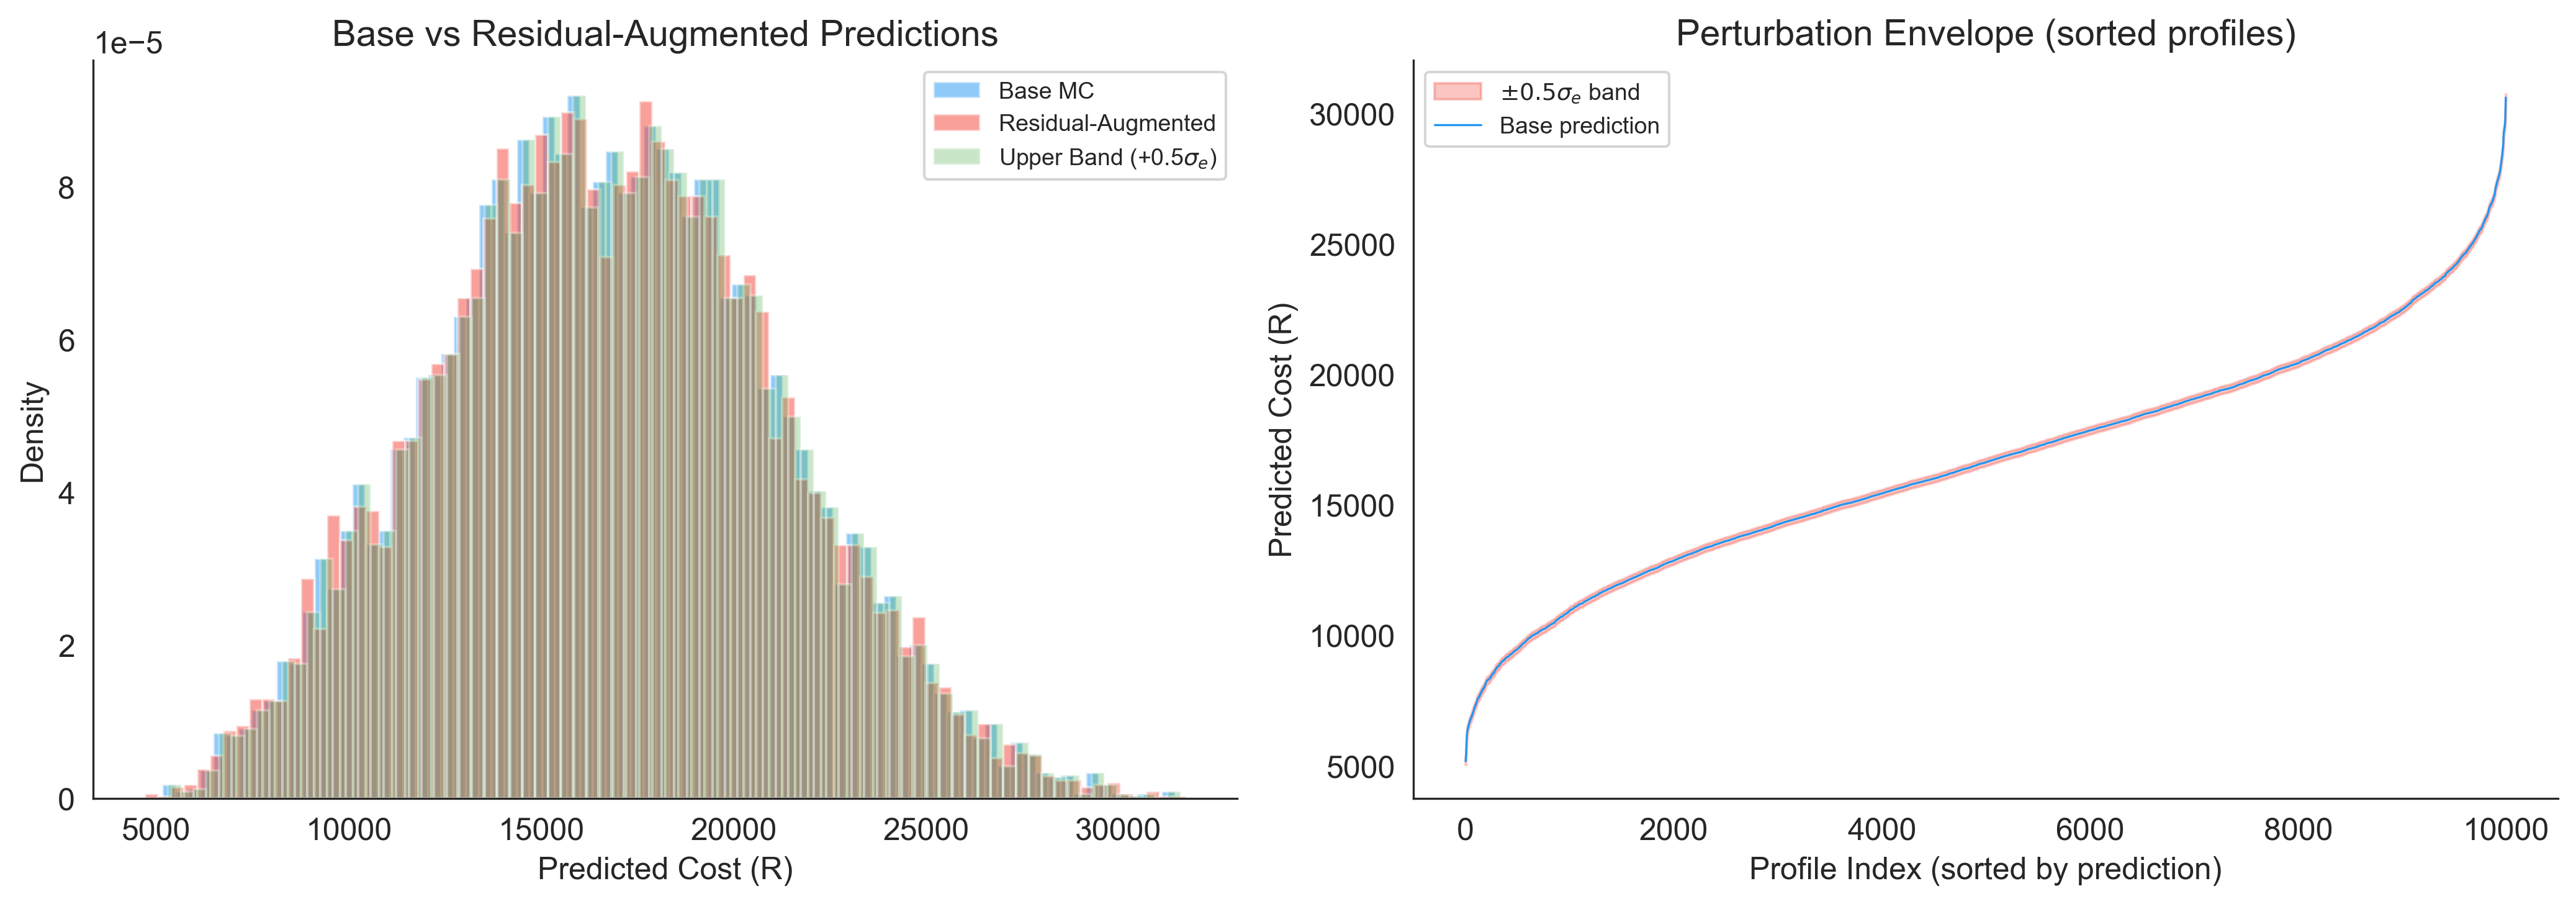
\includegraphics[width=0.95\textwidth]{Thesis/Chapter 4/Figures/fig_mc_residual_augmented.png}
\caption{Residual-augmented Monte Carlo sensitivity analysis.}
\label{fig:mc_residual_augmented_ch4}
\end{figure}

\noindent
Figure~\ref{fig:mc_residual_augmented_ch4} (left panel) shows that the
residual-augmented distribution closely overlaps the base Monte Carlo
distribution. The residual perturbation does not shift the central
tendency or materially alter the distributional shape: the mode, spread
and tail behaviour of all three distributions remain aligned. The right
panel displays the sorted base predictions with the
$\pm 0.5\,\widehat{\sigma}_{\varepsilon}$ perturbation envelope. The
envelope forms a narrow, uniform band around the base prediction curve
across the full range of predicted costs, from approximately R5\,000 at
the lower end to R30\,000 at the upper end. The width of the band
remains constant relative to the prediction magnitude, confirming that
the fitted residual variability is small and homogeneous across the
predicted-cost range.

These results indicate that the distributional conclusions drawn from
the base Monte Carlo analysis are not sensitive to the magnitude of the
fitted model's residual error. The base predicted-cost distribution is
therefore a stable foundation for the Shapley-value attribution analysis
that follows.


% =============================================================
\subsection{Shapley-Value Attribution Results}
\label{sec:shapley_results}

Shapley values were computed for all $B = 10\,000$ simulated
profiles using the gradient-based SHAP explainer described in
Table~\ref{tab:shap_implementation_settings_ch3}. Dummy-level
attributions were aggregated to the raw-variable level ($q = 11$)
using equation~\eqref{eq:raw_variable_shap_aggregation_ch3}.

\subsubsection{Global feature importance}

Global feature importance was assessed using the mean absolute Shapley
value $I_g$ (equation~\eqref{eq:mean_absolute_shap_ch3}) and the mean
signed Shapley value $\overline{\phi}_g$
(equation~\eqref{eq:mean_signed_shap_ch3}), computed over all $B$
simulated profiles.

\begin{figure}[H]
\centering
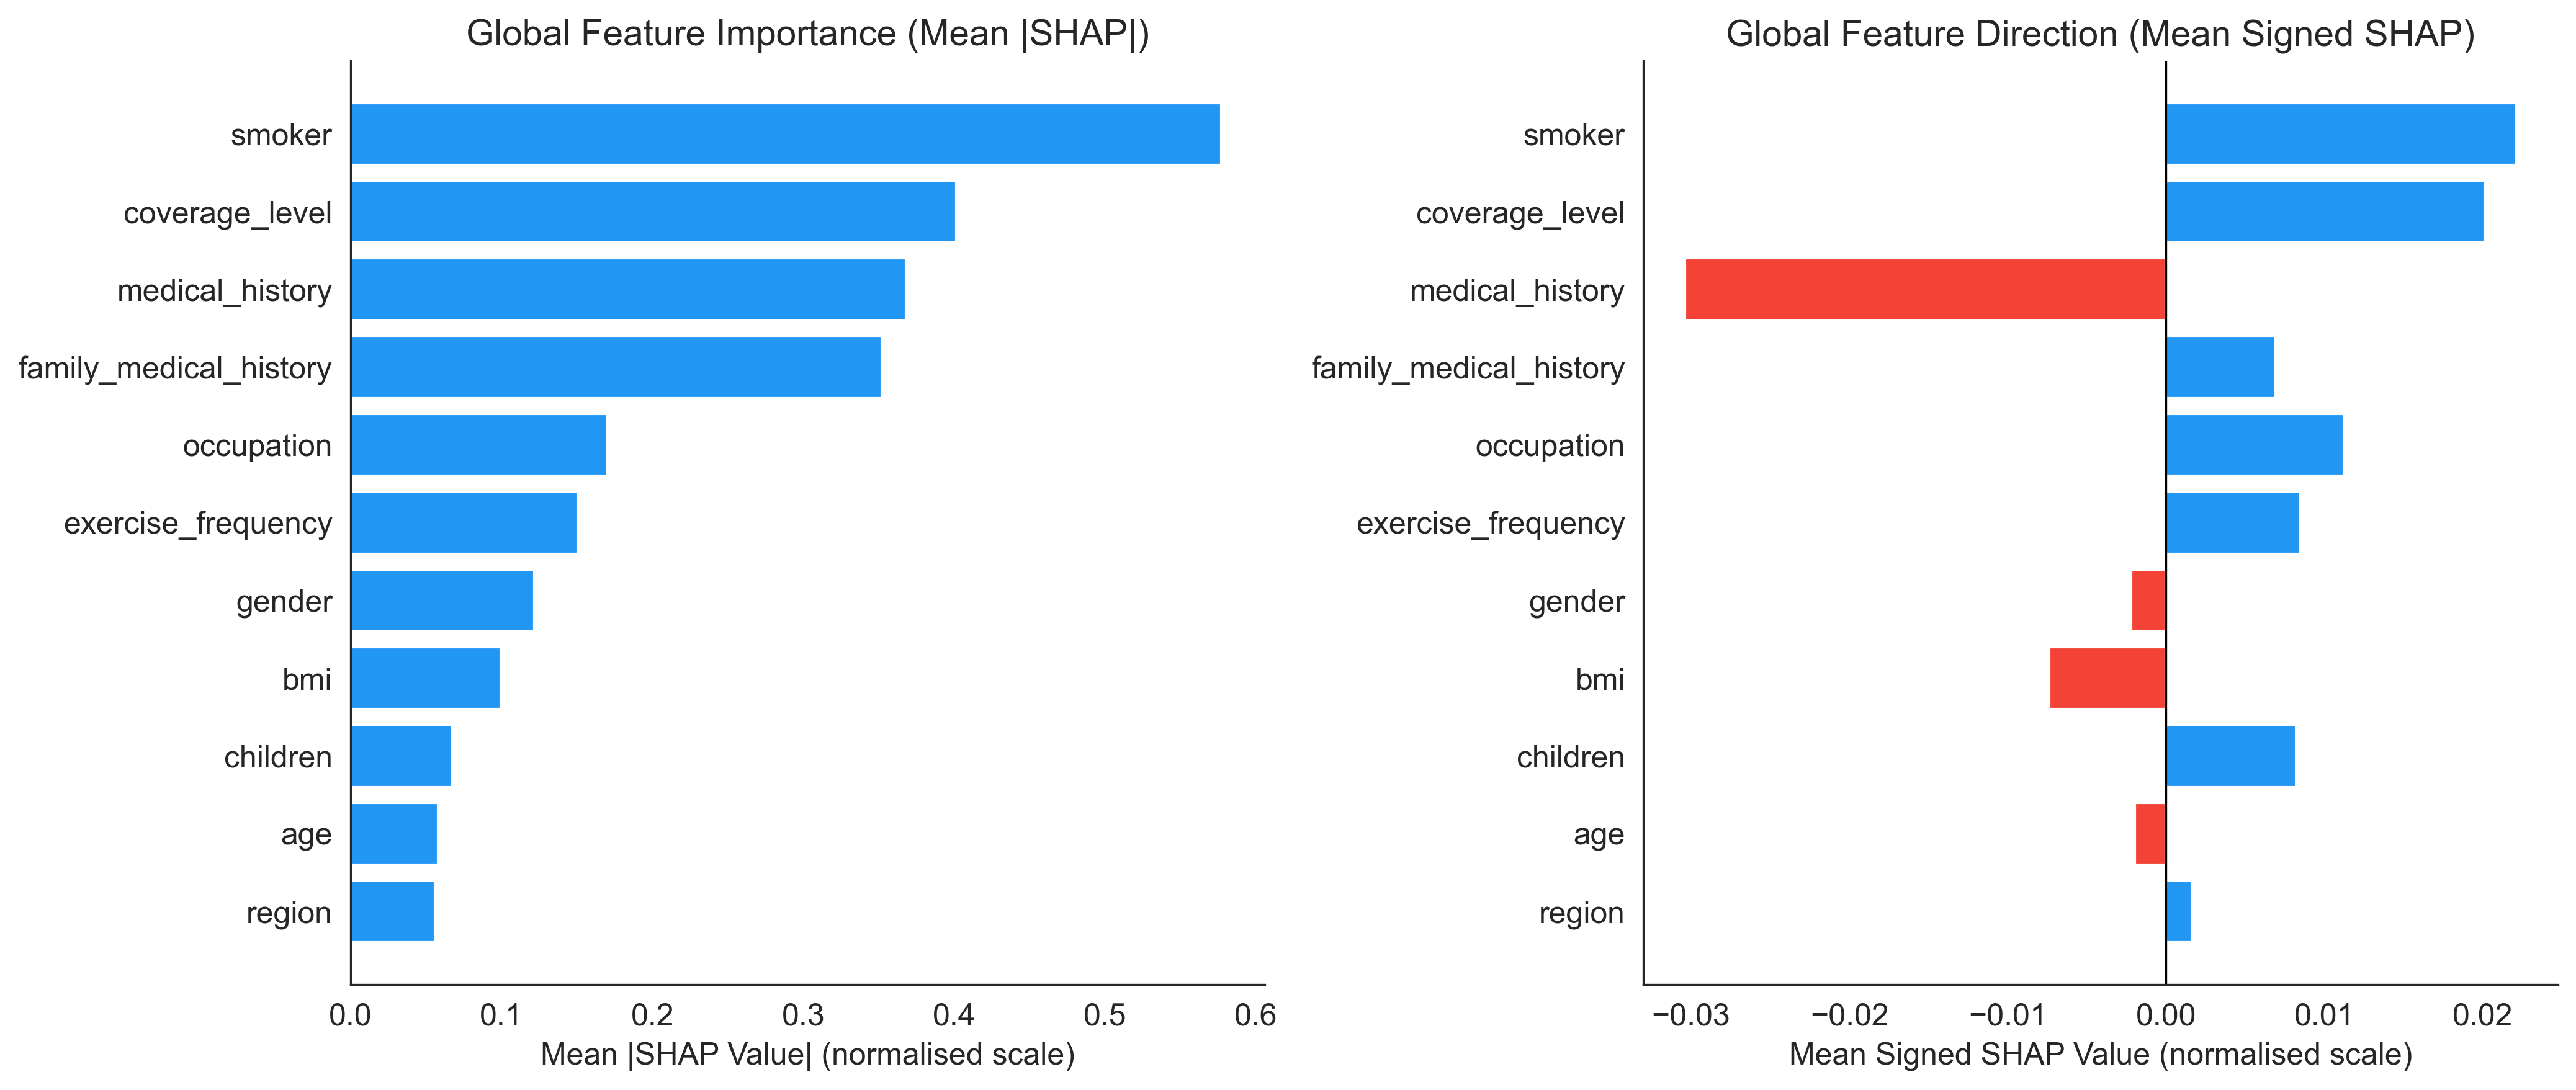
\includegraphics[width=0.95\textwidth]{Thesis/Chapter 4/Figures/fig_shap_global_importance.png}
\caption{Global Shapley feature importance for all 11 raw variables.}
\label{fig:shap_global_importance_ch4}
\end{figure}

\noindent
Figure~\ref{fig:shap_global_importance_ch4} displays the global
feature-importance ranking. Table~\ref{tab:shap_global_importance_ch4}
reports the numerical values.

\begin{table}[H]
\centering
\caption{Global Shapley feature importance: mean signed and mean
absolute values for all 11 raw variables on the normalised scale.}
\label{tab:shap_global_importance_ch4}
\small
\renewcommand{\arraystretch}{1.15}
\begin{tabular}{lrr}
\toprule
\textbf{Variable} & \textbf{Mean signed SHAP} & \textbf{Mean $|\text{SHAP}|$} \\
\midrule
\texttt{smoker} & $+0.022$ & $0.577$ \\
\texttt{coverage\_level} & $+0.020$ & $0.401$ \\
\texttt{medical\_history} & $-0.030$ & $0.368$ \\
\texttt{family\_medical\_history} & $+0.007$ & $0.352$ \\
\texttt{occupation} & $+0.011$ & $0.170$ \\
\texttt{exercise\_frequency} & $+0.009$ & $0.151$ \\
\texttt{gender} & $-0.002$ & $0.122$ \\
\texttt{bmi} & $-0.007$ & $0.099$ \\
\texttt{children} & $+0.008$ & $0.068$ \\
\texttt{age} & $-0.002$ & $0.058$ \\
\texttt{region} & $+0.002$ & $0.056$ \\
\bottomrule
\end{tabular}
\end{table}

\noindent
The four most important variables form a clear top tier:
\texttt{smoker} ($I_g = 0.577$), \texttt{coverage\_level} ($0.401$),
\texttt{medical\_history} ($0.368$) and
\texttt{family\_medical\_history} ($0.352$). These four variables
together account for the large majority of the fitted model's
attribution magnitude. A second tier of moderate contributors includes
\texttt{occupation} ($0.170$) and \texttt{exercise\_frequency}
($0.151$). The remaining five variables (\texttt{gender},
\texttt{bmi}, \texttt{children}, \texttt{age} and \texttt{region})
each have mean $|\text{SHAP}|$ values below $0.13$.

The mean signed values are close to zero for all variables, indicating
that the positive and negative Shapley contributions approximately
cancel out across the simulated profiles. The largest signed value in
absolute terms is \texttt{medical\_history} ($-0.030$), reflecting a
mild directional asymmetry in how the model attributes cost to different
medical history categories.

\subsubsection{Feature-level SHAP beeswarm}

\begin{figure}[H]
\centering
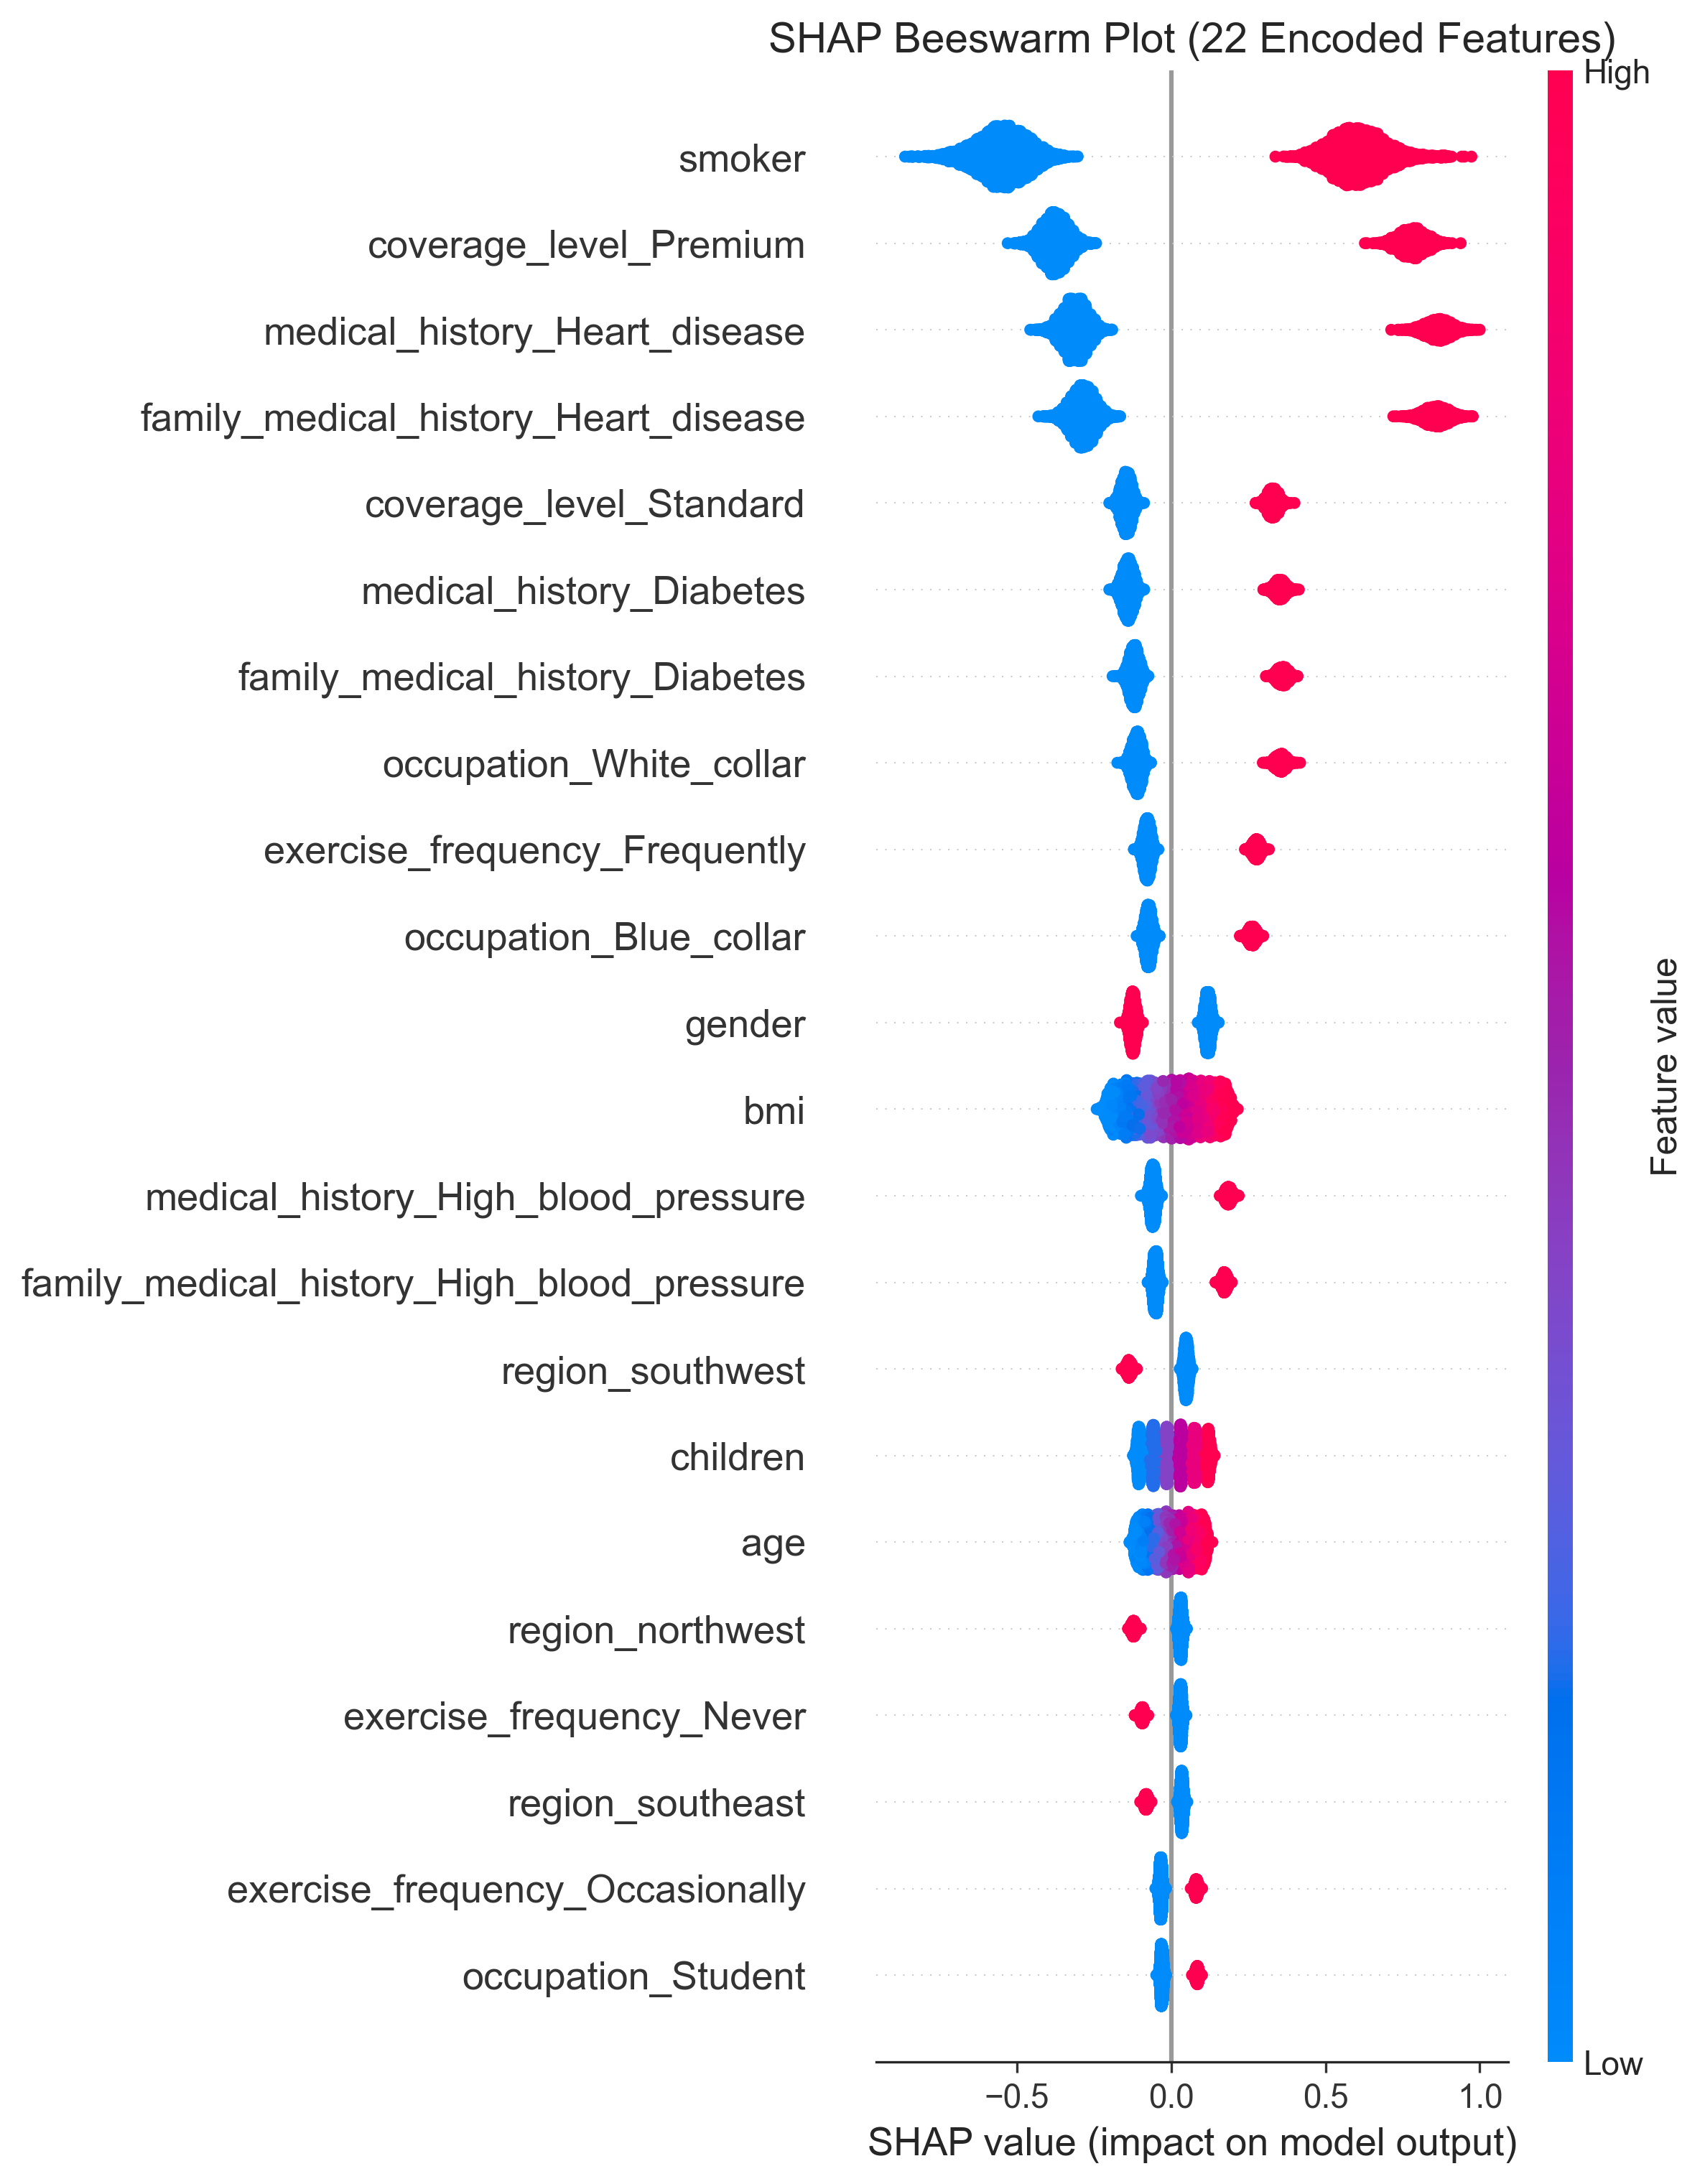
\includegraphics[width=0.72\textwidth]{Thesis/Chapter 4/Figures/fig_shap_beeswarm.png}
\caption{SHAP beeswarm plot for all 22 encoded features.}
\label{fig:shap_beeswarm_ch4}
\end{figure}

\noindent
Figure~\ref{fig:shap_beeswarm_ch4} provides a feature-level view of
the Shapley attributions across all 22 encoded inputs. Several patterns
are visible:

\begin{enumerate}
    \item \textbf{Smoker:} The binary \texttt{smoker} variable produces
    a clear bimodal separation. High feature values (red, smoker $=$ yes)
    yield large positive SHAP values (approximately $+0.5$ to $+1.0$),
    while low feature values (blue, smoker $=$ no) yield large negative
    SHAP values (approximately $-0.5$ to $-0.7$). This confirms that
    smoking status is the single largest determinant of fitted predicted
    costs.

    \item \textbf{Coverage level:} The \texttt{coverage\_level\_Premium}
    dummy exhibits a similar bimodal pattern: premium coverage pushes
    predictions upward ($+0.3$ to $+0.7$), while its absence pulls
    predictions downward. The \texttt{coverage\_level\_Standard} dummy
    shows a complementary pattern of smaller magnitude.

    \item \textbf{Medical and family medical history:} The Heart disease
    dummies for both \texttt{medical\_history} and
    \texttt{family\_medical\_history} produce the next largest
    attributions. High feature values (Heart disease present)
    consistently increase predicted costs by approximately $+0.3$ to
    $+0.8$.

    \item \textbf{Continuous variables:} \texttt{bmi}, \texttt{children}
    and \texttt{age} display more diffuse SHAP distributions centred
    near zero, consistent with their smaller global importance. The
    \texttt{bmi} swarm shows a broad purple-to-pink gradient, reflecting
    its continuous nature, but the individual SHAP magnitudes remain
    small (mostly within $\pm 0.15$).
\end{enumerate}

\subsubsection{Training versus Monte Carlo attribution invariance}

\begin{figure}[H]
\centering
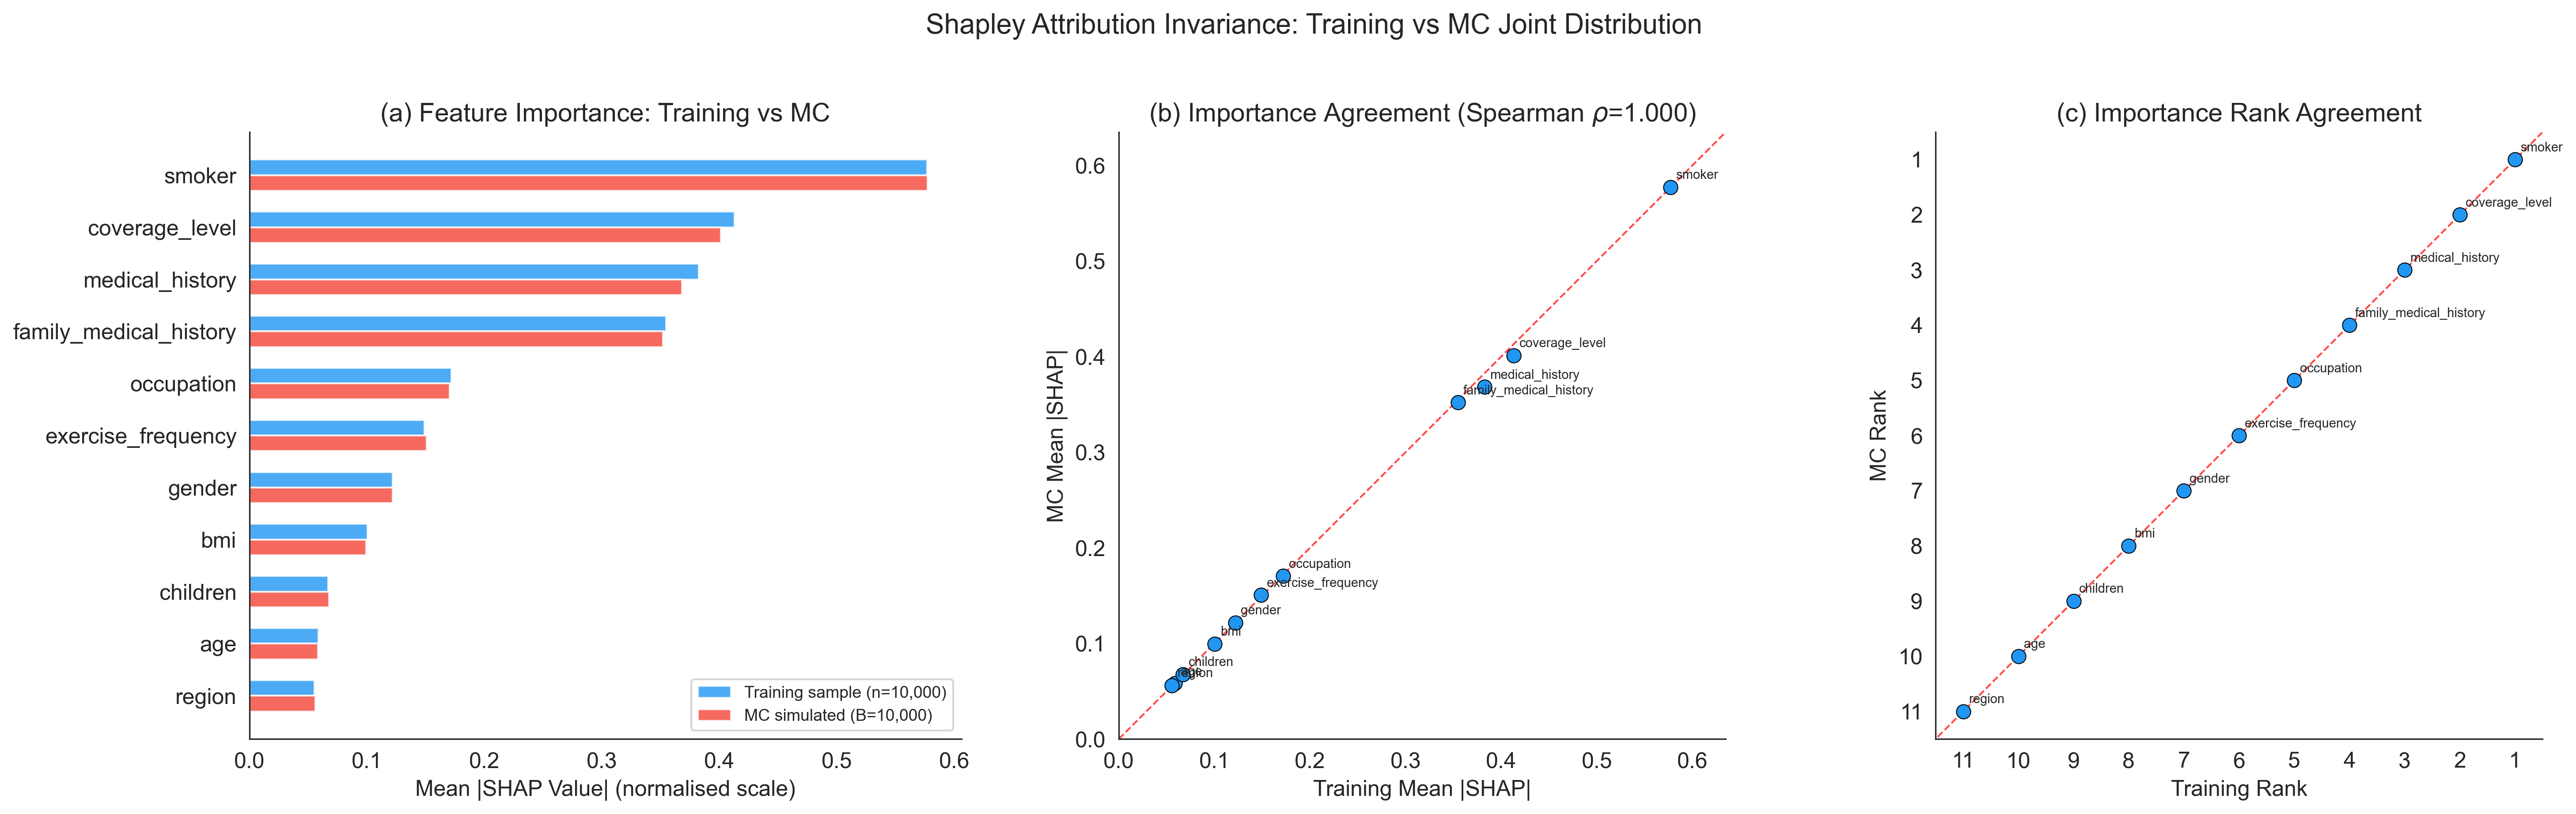
\includegraphics[width=0.95\textwidth]{Thesis/Chapter 4/Figures/fig_shap_training_vs_mc_invariance.png}
\caption{Shapley attribution invariance: training data versus Monte Carlo profiles.}
\label{fig:shap_training_vs_mc_invariance_ch4}
\end{figure}

\noindent
Figure~\ref{fig:shap_training_vs_mc_invariance_ch4} compares the
Shapley attributions computed on the training data with those computed on
the Monte Carlo simulated profiles. The Spearman rank correlation
between the two feature-importance vectors is $\rho_{\mathrm{S}} =
1.000$: all 11 raw variables occupy the same importance rank under both
input regimes. The scatter plot in panel~(b) shows that the mean
$|\text{SHAP}|$ values fall on the diagonal, with no systematic
deviation. This result extends the parametric-versus-bootstrap invariance
finding of Section~\ref{sec:mc_input_validation} (Spearman
$\rho = 0.991$) and confirms that the fitted \gls{dnn}'s internal
feature-importance structure is preserved when evaluated on the Monte
Carlo simulated input space.


% =============================================================
\subsection{High-Cost Conditional Shapley Analysis}
\label{sec:highcost_conditional_results}

The high-cost region was defined using the quantile-based thresholds
$u_{\tau}$ (equation~\eqref{eq:high_cost_threshold}) applied to the
Monte Carlo predicted-cost distribution.
Table~\ref{tab:highcost_thresholds_ch4} reports the three threshold
values and the corresponding high-cost set sizes.

\begin{table}[H]
\centering
\caption{High-cost thresholds from the Monte Carlo predicted-cost
distribution.}
\label{tab:highcost_thresholds_ch4}
\small
\renewcommand{\arraystretch}{1.15}
\begin{tabular}{lrrrr}
\toprule
\textbf{Threshold} & $\boldsymbol{\tau}$ &
$\boldsymbol{u_{\tau}}$ \textbf{(R)} &
$\boldsymbol{|\mathcal{H}_{\tau}|}$ &
\textbf{Proportion} \\
\midrule
$\tau_{90}$ & 0.90 & 22\,482 & 1\,000 & 0.10 \\
$\tau_{95}$ & 0.95 & 24\,154 & 500 & 0.05 \\
$\tau_{99}$ & 0.99 & 27\,160 & 100 & 0.01 \\
\bottomrule
\end{tabular}
\end{table}

\subsubsection{Conditional versus global importance}

Conditional mean absolute Shapley values were computed for profiles in
$\mathcal{H}_{\tau}$ at each threshold and compared with the global
values.

\begin{figure}[H]
\centering
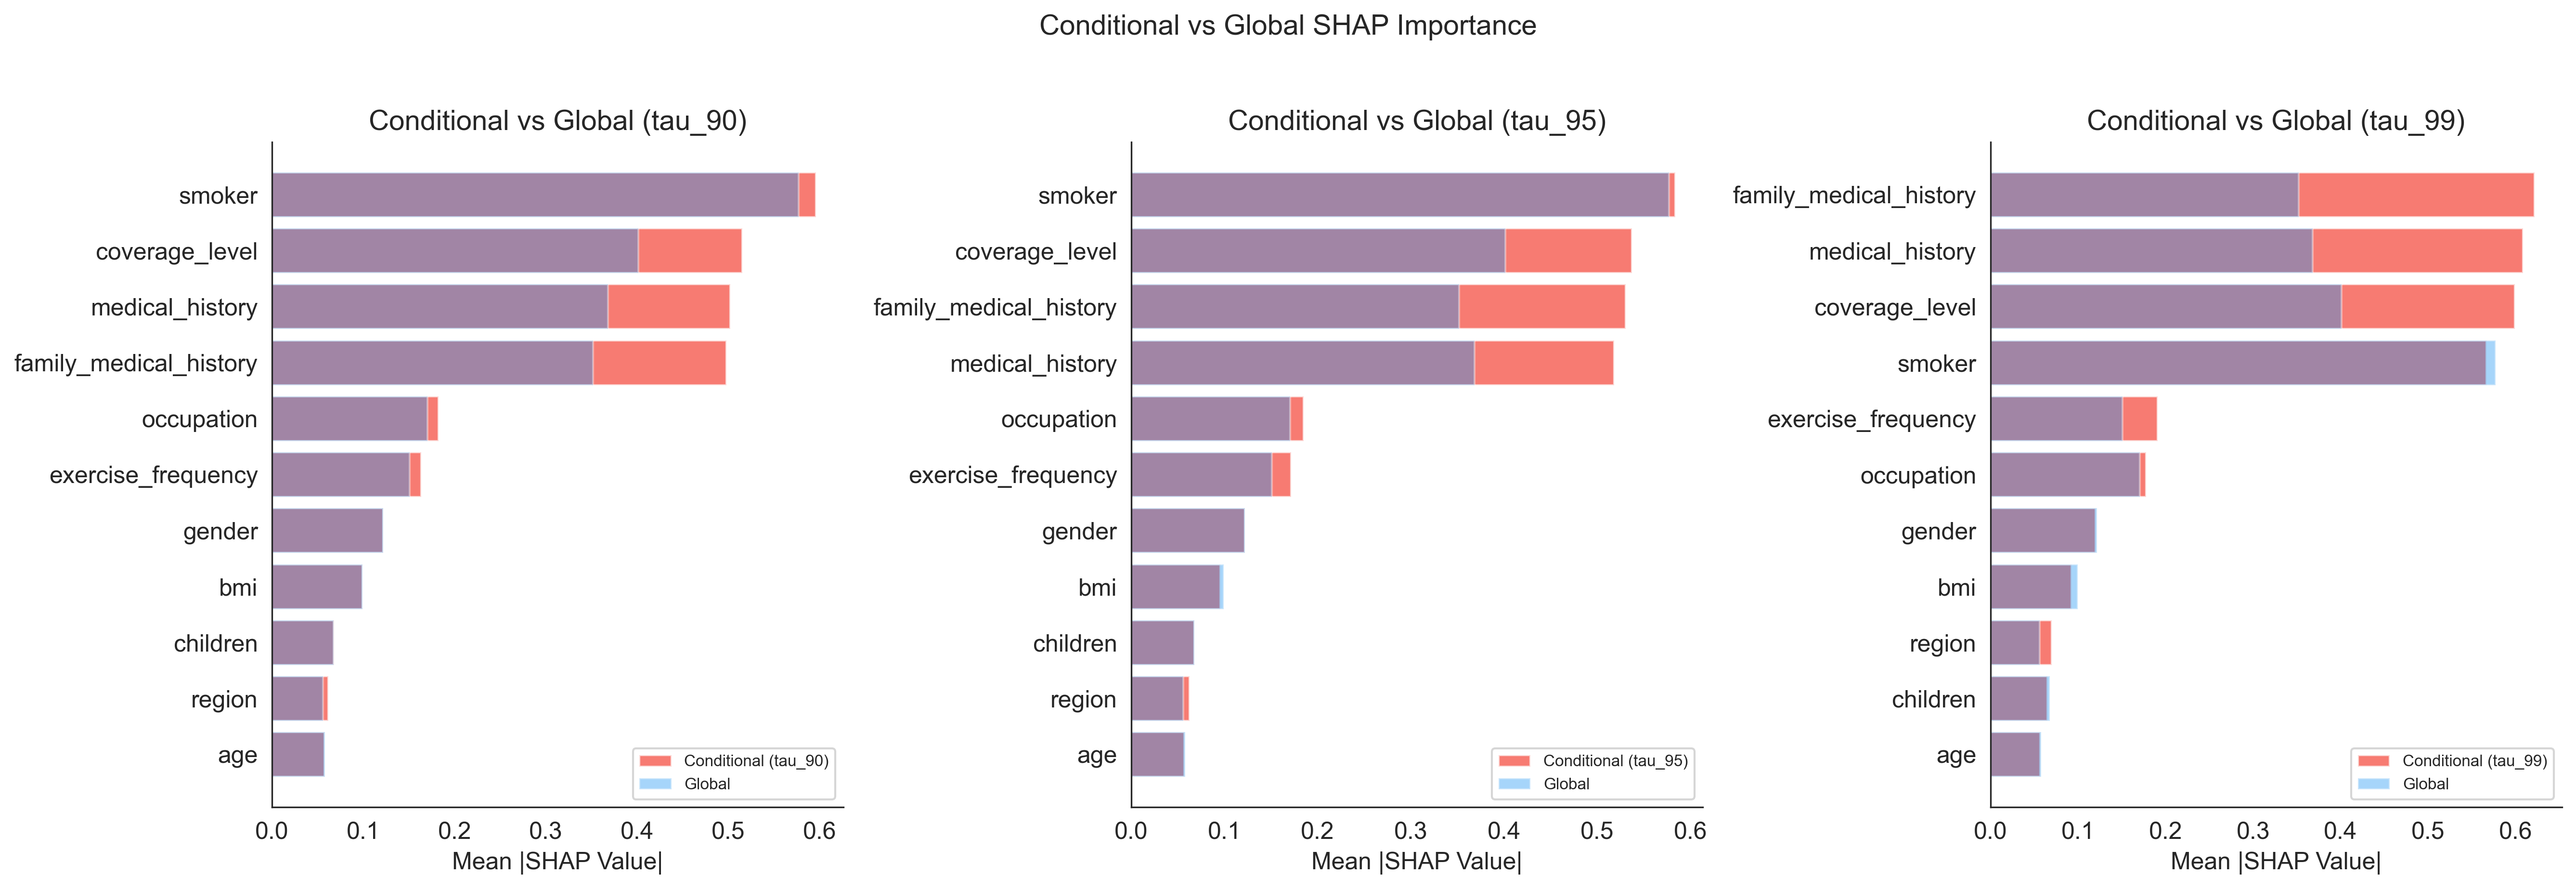
\includegraphics[width=0.95\textwidth]{Thesis/Chapter 4/Figures/fig_shap_conditional_importance.png}
\caption{Conditional versus global mean $|\text{SHAP}|$ importance at three upper-tail thresholds.}
\label{fig:shap_conditional_importance_ch4}
\end{figure}

\noindent
Figure~\ref{fig:shap_conditional_importance_ch4} reveals a progressive
shift in the feature-importance ranking as the threshold moves into the
extreme upper tail:

\begin{itemize}
    \item At $\tau_{90}$, the ranking mirrors the global ordering:
    \texttt{smoker} remains the most important variable, followed by
    \texttt{coverage\_level}, \texttt{medical\_history} and
    \texttt{family\_medical\_history}. The conditional importance values
    are slightly higher than the global values for the top four
    variables, reflecting the more extreme nature of the high-cost
    profiles.

    \item At $\tau_{95}$, the top four variables maintain similar
    positions, but \texttt{family\_medical\_history} and
    \texttt{medical\_history} show increased conditional importance
    relative to their global values.

    \item At $\tau_{99}$, a ranking reversal occurs:
    \texttt{family\_medical\_history} ($I_{g,0.99} = 0.622$) and
    \texttt{medical\_history} ($I_{g,0.99} = 0.608$) overtake
    \texttt{smoker} ($I_{g,0.99} = 0.566$) as the most important
    variables. \texttt{coverage\_level} ($I_{g,0.99} = 0.599$) also
    exceeds \texttt{smoker} in the extreme tail.
\end{itemize}

\noindent
Table~\ref{tab:shap_conditional_values_ch4} reports the conditional
mean $|\text{SHAP}|$ values at all three thresholds alongside the global
values.

\begin{table}[H]
\centering
\caption{Mean absolute Shapley values: global and conditional at each
high-cost threshold (normalised scale).}
\label{tab:shap_conditional_values_ch4}
\small
\renewcommand{\arraystretch}{1.15}
\begin{tabular}{lrrrr}
\toprule
\textbf{Variable} & \textbf{Global} & $\boldsymbol{\tau_{90}}$ &
$\boldsymbol{\tau_{95}}$ & $\boldsymbol{\tau_{99}}$ \\
\midrule
\texttt{smoker} & 0.577 & 0.596 & 0.584 & 0.566 \\
\texttt{coverage\_level} & 0.401 & 0.515 & 0.537 & 0.599 \\
\texttt{medical\_history} & 0.368 & 0.502 & 0.518 & 0.608 \\
\texttt{family\_medical\_history} & 0.352 & 0.498 & 0.531 & 0.622 \\
\texttt{occupation} & 0.170 & 0.183 & 0.185 & 0.178 \\
\texttt{exercise\_frequency} & 0.151 & 0.164 & 0.171 & 0.191 \\
\texttt{gender} & 0.122 & 0.122 & 0.122 & 0.120 \\
\texttt{bmi} & 0.099 & 0.099 & 0.095 & 0.092 \\
\texttt{children} & 0.068 & 0.068 & 0.068 & 0.065 \\
\texttt{age} & 0.058 & 0.058 & 0.057 & 0.057 \\
\texttt{region} & 0.056 & 0.062 & 0.062 & 0.070 \\
\bottomrule
\end{tabular}
\end{table}

\subsubsection{Threshold stability of the importance ranking}

\begin{figure}[H]
\centering
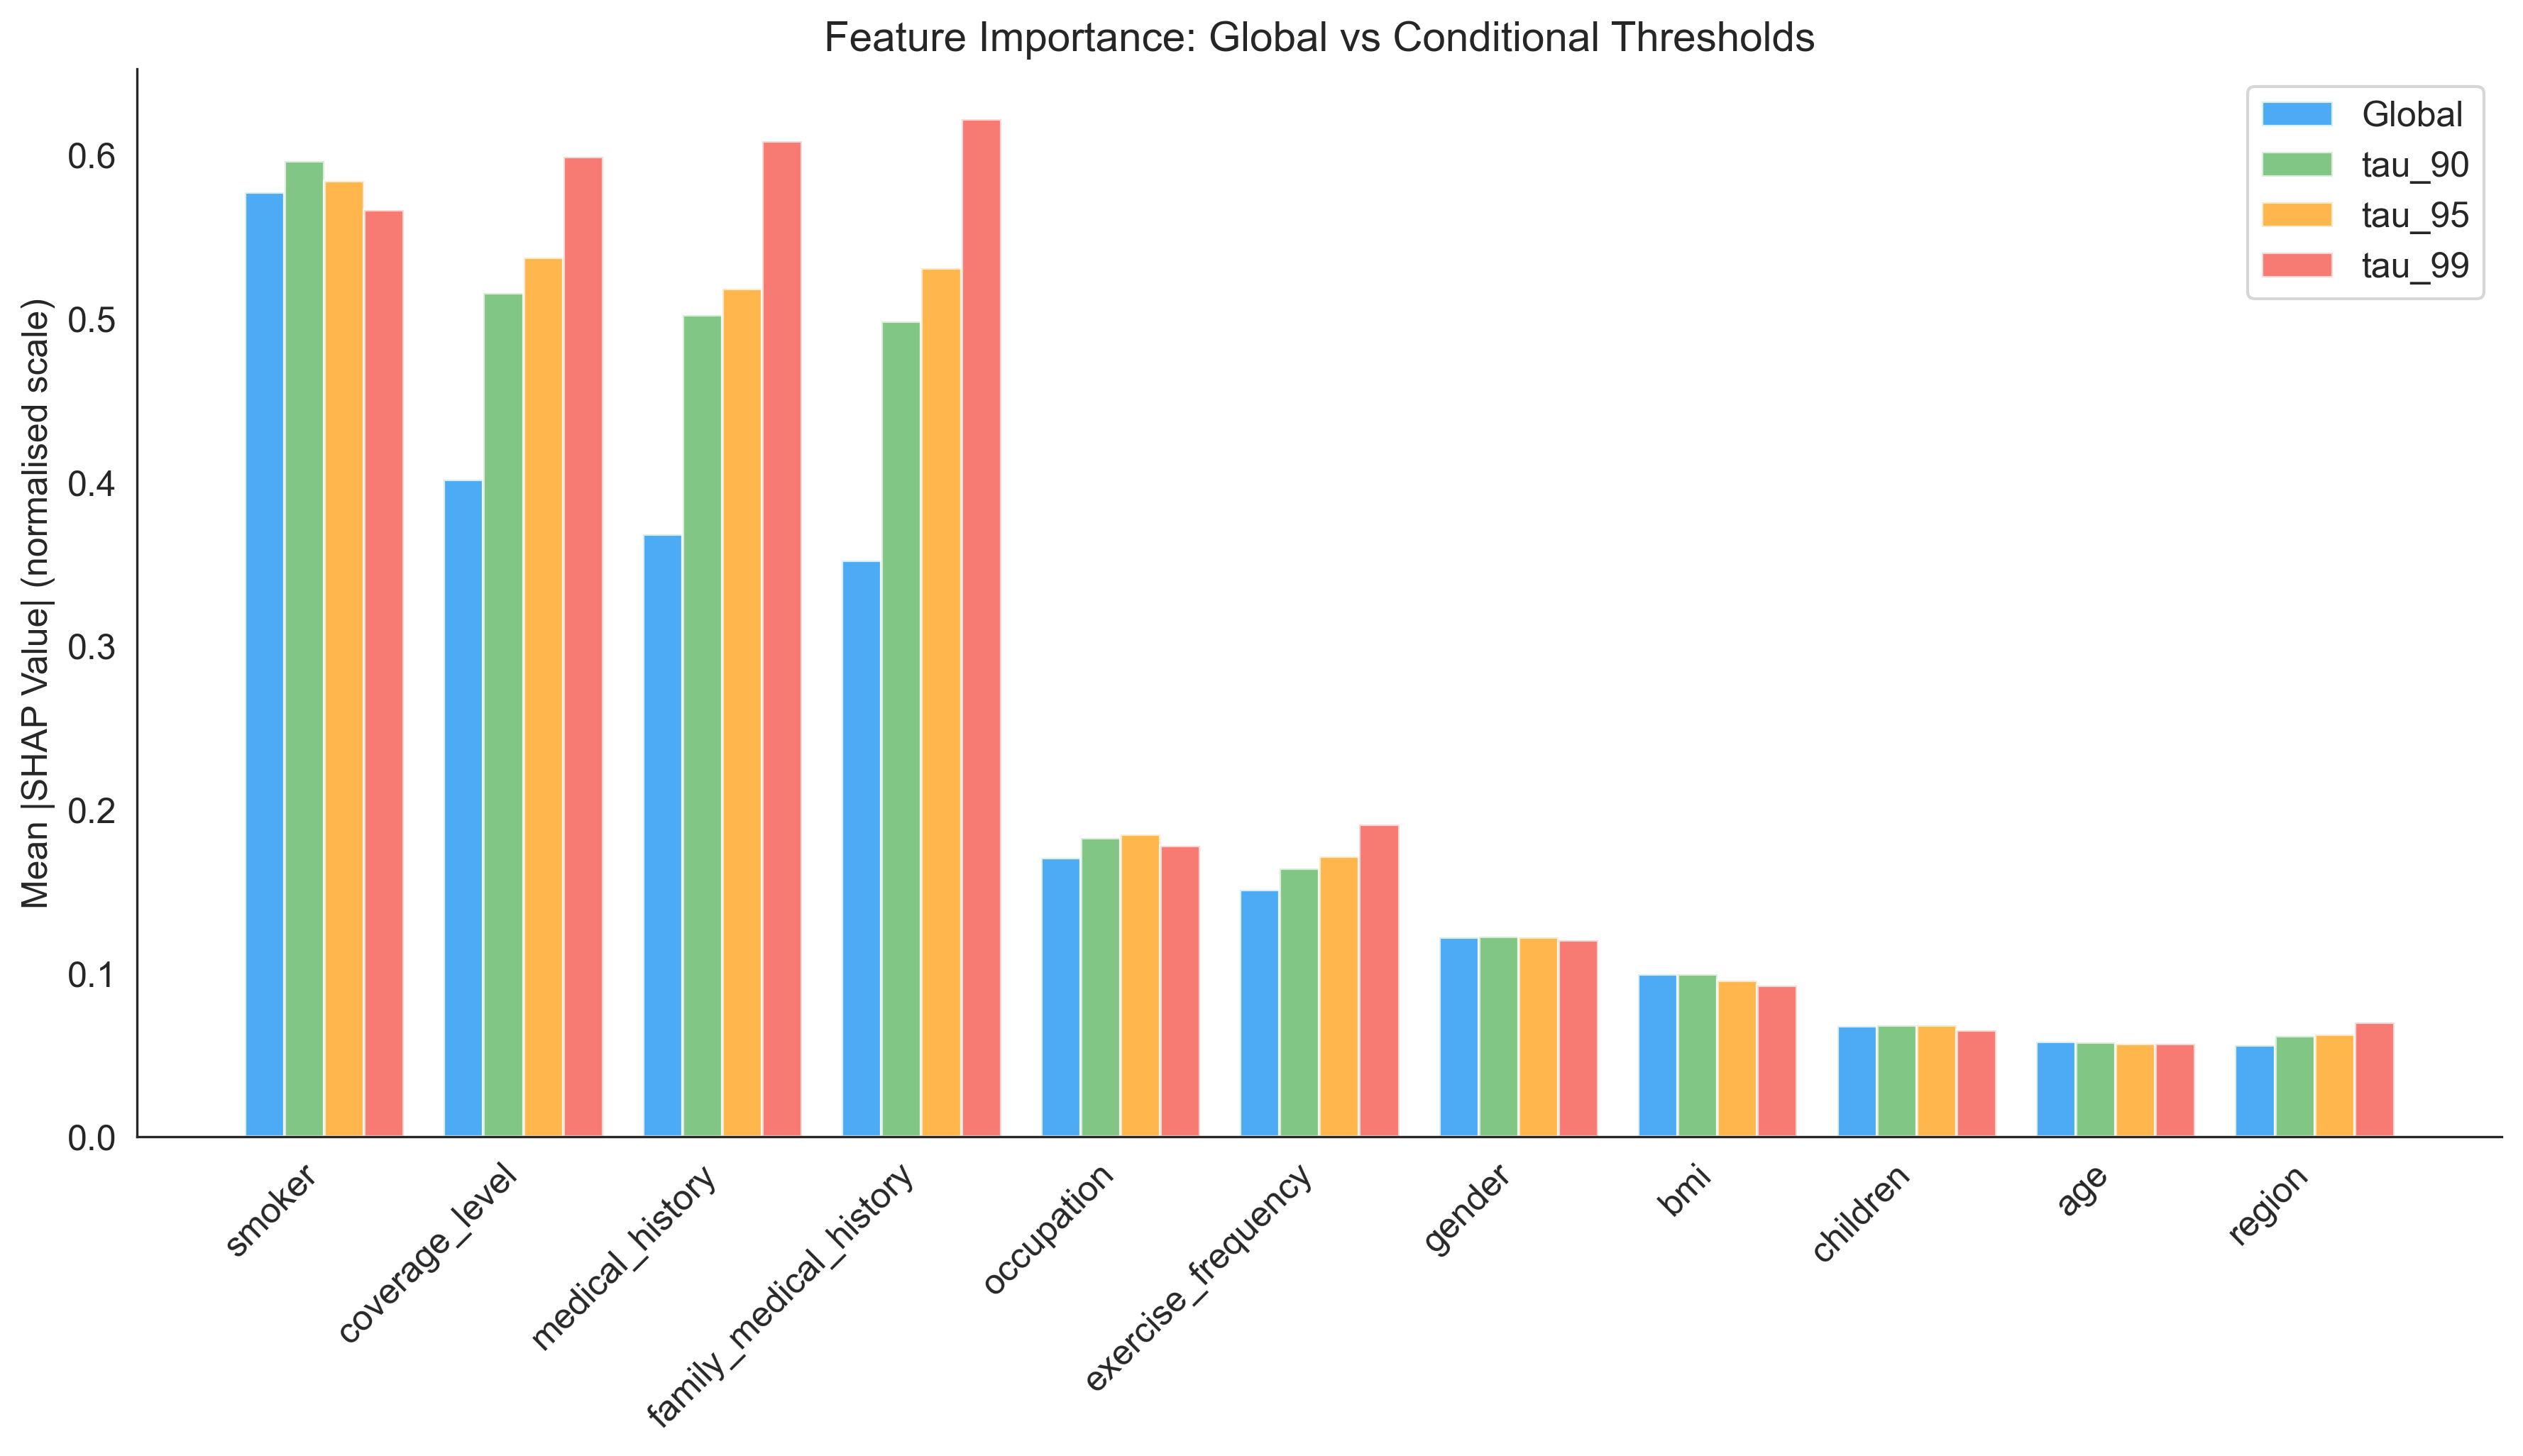
\includegraphics[width=0.85\textwidth]{Thesis/Chapter 4/Figures/fig_shap_threshold_comparison.png}
\caption{Feature importance across thresholds: mean $|\text{SHAP}|$
values at the global, $\tau_{90}$, $\tau_{95}$ and $\tau_{99}$ levels
for all 11 raw variables.}
\label{fig:shap_threshold_comparison_ch4}
\end{figure}

\noindent
Figure~\ref{fig:shap_threshold_comparison_ch4} displays the
threshold-comparison bar chart. The dominant pattern is a monotonic
increase in the conditional importance of
\texttt{coverage\_level}, \texttt{medical\_history} and
\texttt{family\_medical\_history} as the threshold moves from the global
level through $\tau_{90}$ and $\tau_{95}$ to $\tau_{99}$. In contrast,
\texttt{smoker} shows a slight decline in conditional importance at the
most extreme threshold ($0.566$ at $\tau_{99}$ versus $0.577$ globally).
This decline does not indicate that smoking status becomes
unimportant; rather, it reflects a ceiling effect: nearly all profiles
in the extreme upper tail are smokers (as confirmed in
Figure~\ref{fig:highcost_profiles_ch4} below), so the binary variable
contributes a near-constant positive attribution with reduced
variability, while the remaining features differentiate among the
high-cost profiles.

The second tier of variables (\texttt{occupation},
\texttt{exercise\_frequency}, \texttt{gender}, \texttt{bmi},
\texttt{children}, \texttt{age} and \texttt{region}) remains stable
across all thresholds, with conditional importance values close to
their global values. This stability indicates that these variables
contribute a consistent baseline attribution regardless of the cost
region.

The ranking reversal at $\tau_{99}$ directly addresses the research gap
identified in Section~\ref{sec:research_gap}: existing health-cost
prediction studies typically report global feature importance on observed
data only \citep{kaushik2022machine, rozemberczki2022shapley}, without
conditioning attributions on specific regions of the predicted-cost
distribution.  The conditional Shapley analysis demonstrates that global
importance rankings can be misleading when the interest lies in the
upper tail, because a variable that dominates on average (smoking status)
may lose its discriminating power within an extreme subpopulation where
it is nearly constant.  This distinction has not been documented in the
health insurance cost-prediction literature reviewed in
Chapter~\ref{sec:literature_review}.

\subsubsection{High-cost profile characteristics}

\begin{figure}[H]
\centering
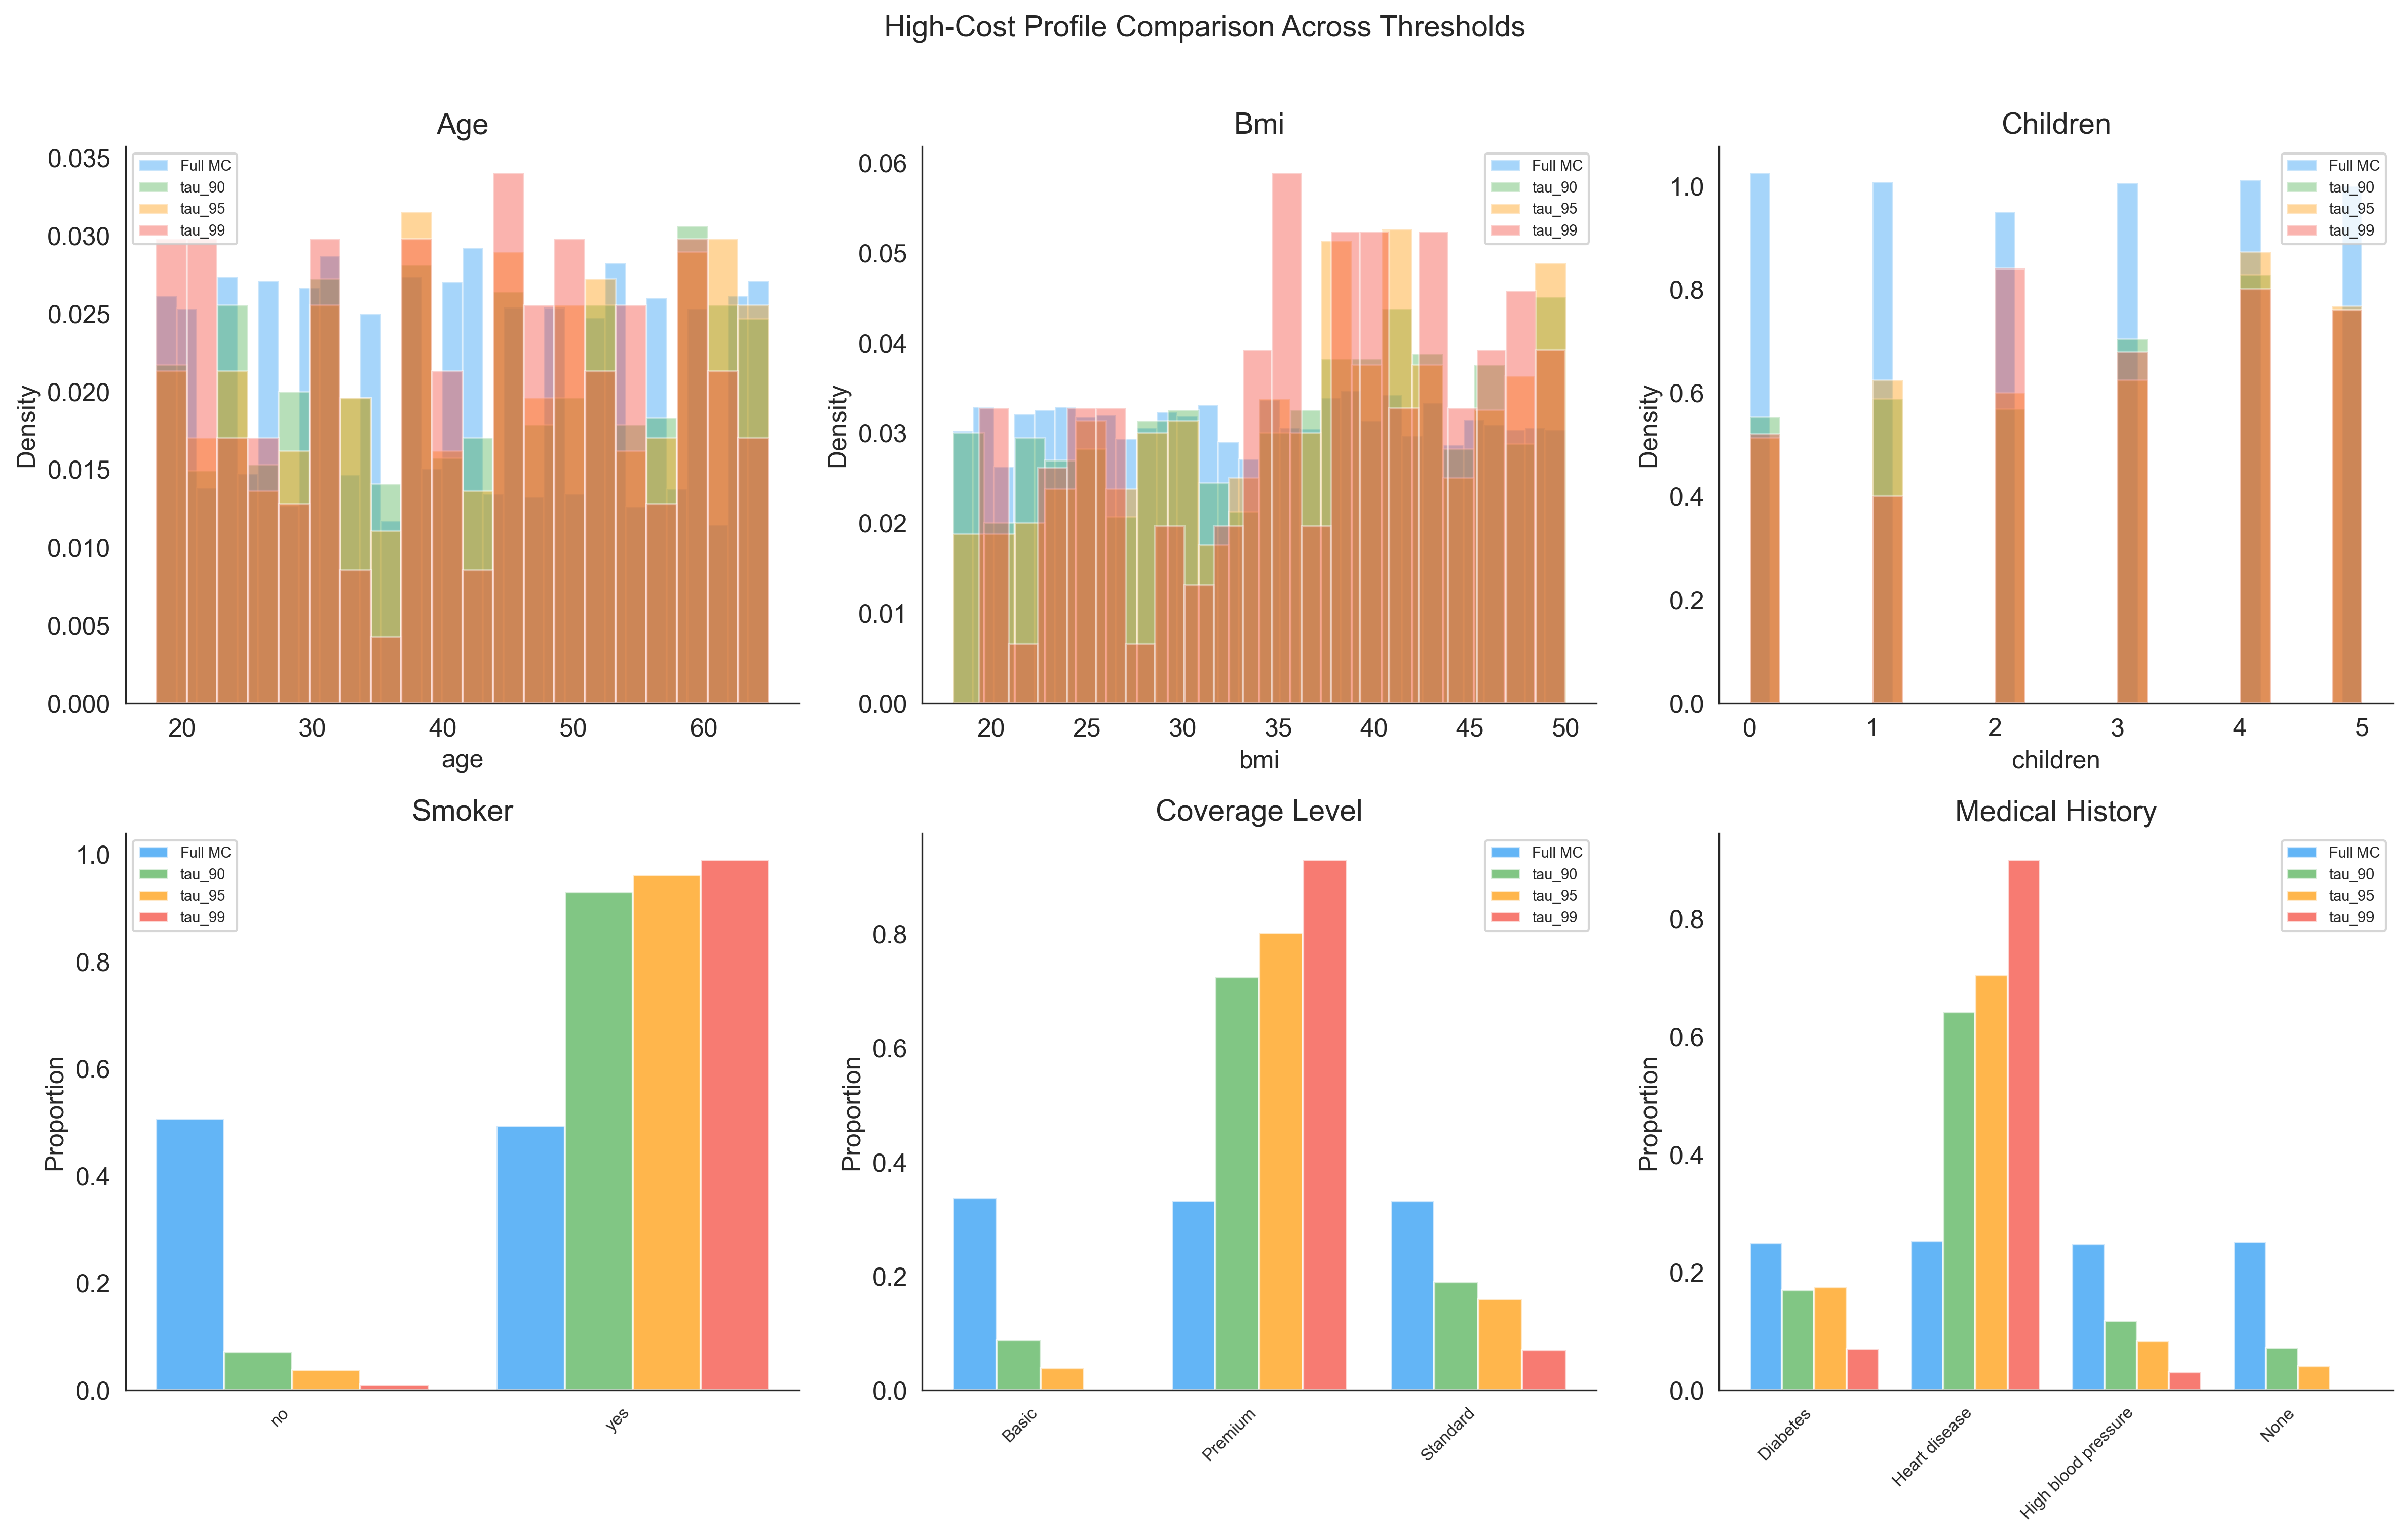
\includegraphics[width=0.95\textwidth]{Thesis/Chapter 4/Figures/fig_highcost_profile_comparison.png}
\caption{Distributional profiles of the high-cost sets compared with the full Monte Carlo sample.}
\label{fig:highcost_profiles_ch4}
\end{figure}

\noindent
Figure~\ref{fig:highcost_profiles_ch4} profiles the composition of the
high-cost sets at each threshold. The categorical panels reveal a
progressive concentration:

\begin{itemize}
    \item \textbf{Smoker:} The proportion of smokers increases from
    approximately $50\%$ in the full Monte Carlo sample to approximately
    $93\%$ at $\tau_{90}$, $96\%$ at $\tau_{95}$ and $99\%$ at
    $\tau_{99}$. At the most extreme threshold, virtually all high-cost
    profiles are smokers.

    \item \textbf{Coverage level:} The proportion of Premium-tier
    policyholders rises from approximately $33\%$ (full MC) to $75\%$
    at $\tau_{90}$, $80\%$ at $\tau_{95}$ and approximately $90\%$ at
    $\tau_{99}$. Basic-tier policyholders are nearly absent from the
    extreme tail.

    \item \textbf{Medical history:} Heart disease dominates the
    high-cost sets: its proportion increases from approximately $25\%$
    (full MC) to $68\%$ at $\tau_{90}$, $77\%$ at $\tau_{95}$ and
    approximately $85\%$ at $\tau_{99}$. Profiles with no medical
    history condition are progressively excluded from the upper tail.
\end{itemize}

\noindent
The continuous variables (\texttt{age}, \texttt{bmi},
\texttt{children}) show little change in their distributional shapes
across thresholds, consistent with their small and stable conditional
Shapley values. This confirms that the high-cost region is defined
primarily by the categorical risk factors rather than the continuous
covariates.

\subsubsection{Representative high-cost waterfall decomposition}

\begin{figure}[H]
\centering
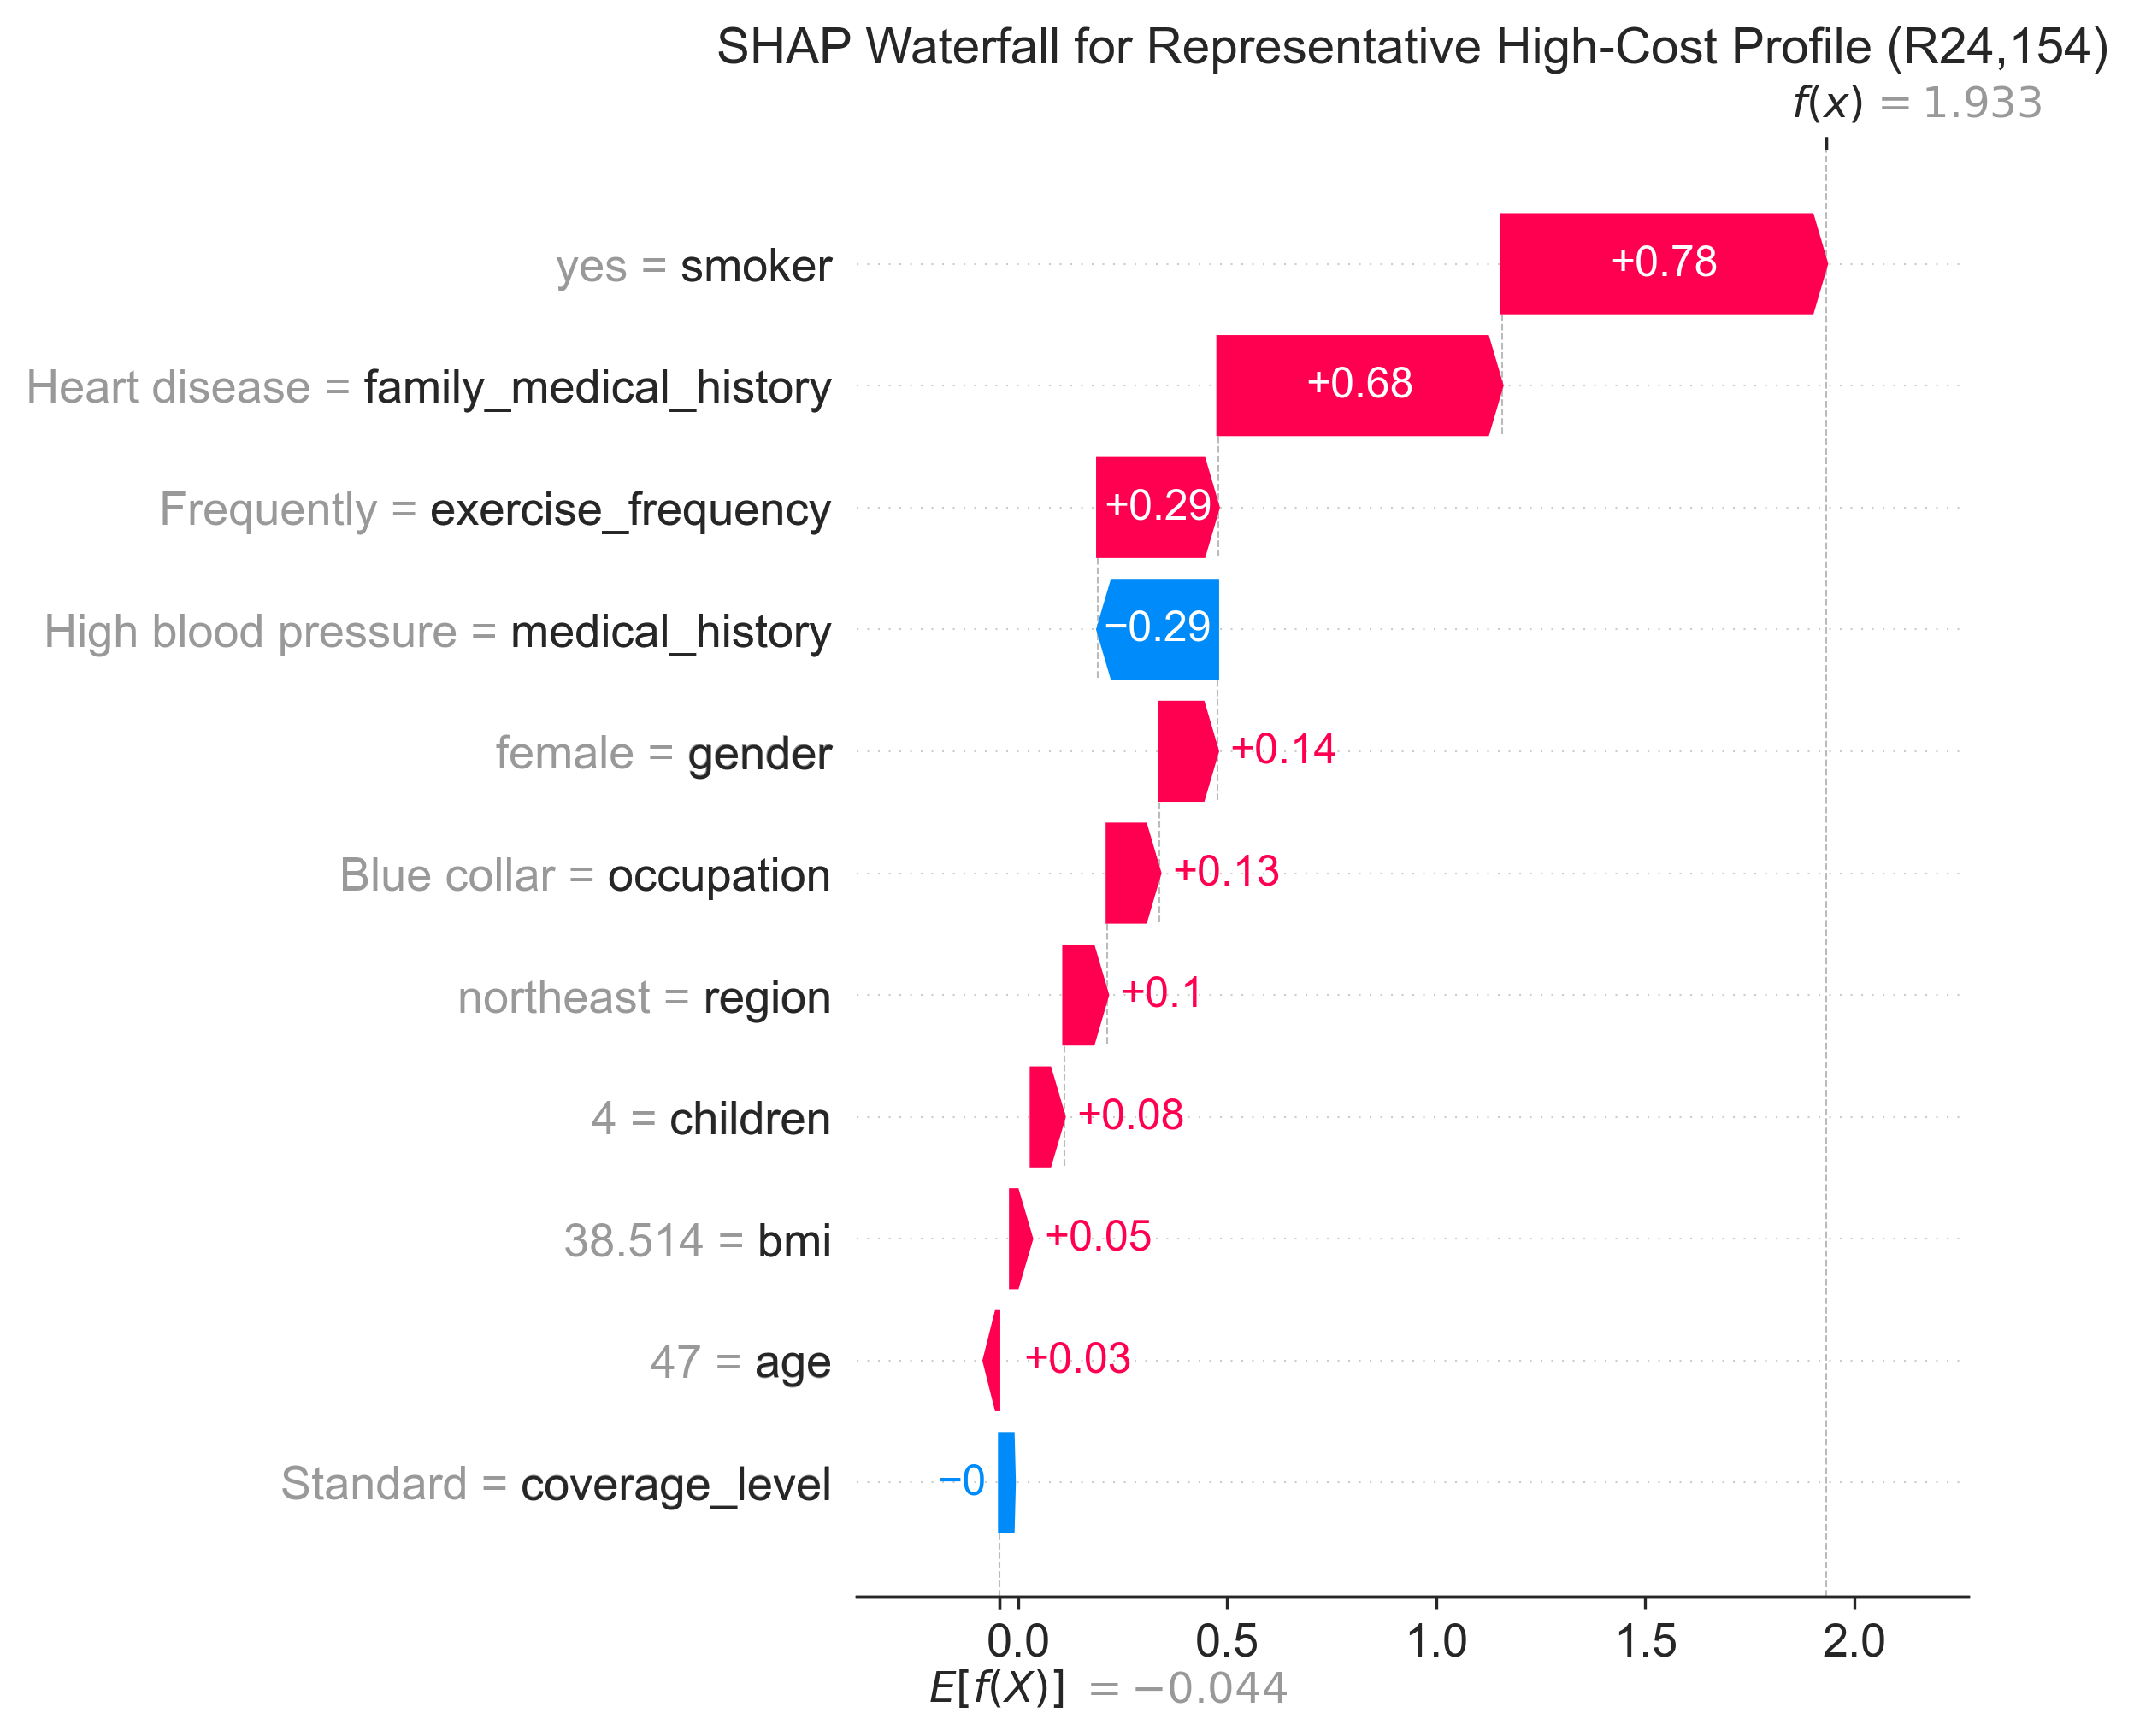
\includegraphics[width=0.75\textwidth]{Thesis/Chapter 4/Figures/fig_shap_highcost_waterfall.png}
\caption{SHAP waterfall plot for a representative high-cost profile
at the $\tau_{95}$ threshold (predicted cost R24\,154).}
\label{fig:shap_waterfall_ch4}
\end{figure}

\noindent
Figure~\ref{fig:shap_waterfall_ch4} decomposes a representative
high-cost profile at the $\tau_{95}$ threshold. The profile has the
following characteristics: age~$= 47$, \texttt{bmi}~$= 38.5$,
\texttt{children}~$= 4$, \texttt{smoker}~$=$ yes,
\texttt{family\_medical\_history}~$=$ Heart disease,
\texttt{exercise\_frequency}~$=$ Frequently,
\texttt{medical\_history}~$=$ High blood pressure,
\texttt{gender}~$=$ female, \texttt{occupation}~$=$ Blue collar,
\texttt{region}~$=$ northeast,
\texttt{coverage\_level}~$=$ Standard.

The waterfall decomposition shows that the prediction is driven upward
from the baseline ($E[f(X)] = -0.044$) to the final prediction
($f(x) = 1.933$) primarily by three variables:
\texttt{smoker} ($+0.78$), \texttt{family\_medical\_history} ($+0.68$)
and \texttt{exercise\_frequency} ($+0.29$). A negative contribution
from \texttt{medical\_history} ($-0.29$) partially offsets these
positive effects, reflecting that High blood pressure carries a lower
attribution than Heart disease within the \texttt{medical\_history}
variable. The remaining variables contribute small positive amounts,
with \texttt{coverage\_level} contributing nearly zero ($-0.00$) because
the Standard tier occupies a middle position in the coverage hierarchy.

This waterfall illustrates the additive decomposition guaranteed by the
Shapley efficiency axiom: the contributions sum exactly to the
difference between the prediction and the baseline, as required by
equation~\eqref{eq:shapley_decomp}.


% =============================================================
\subsection{Integration of Monte Carlo and Shapley Results}
\label{sec:mc_shapley_integration}

The Monte Carlo and Shapley analyses provide complementary perspectives
on the fitted \gls{dnn}'s behaviour. The Monte Carlo simulation
identifies the distributional regions of interest within the
predicted-cost landscape, while the Shapley-value decomposition reveals
which input variables are associated with those regions.

The Monte Carlo predicted-cost distribution
(Figure~\ref{fig:mc_predicted_cost_distribution_ch4}) is approximately
symmetric with a mean of R16\,707 and an upper tail extending to
R31\,466. Within this landscape, three quantile-based thresholds
define high-cost regions of increasing severity:
$u_{0.90} = \text{R22\,482}$, $u_{0.95} = \text{R24\,154}$ and
$u_{0.99} = \text{R27\,160}$.

The global Shapley analysis
(Figure~\ref{fig:shap_global_importance_ch4}) identifies
\texttt{smoker} as the dominant driver of fitted predictions across
the full simulated input space. However, the conditional analysis
(Figures~\ref{fig:shap_conditional_importance_ch4}
and~\ref{fig:shap_threshold_comparison_ch4}) reveals that the
attribution structure changes in the upper tail. As the high-cost
threshold becomes more stringent, the conditional importance of
\texttt{coverage\_level}, \texttt{medical\_history} and
\texttt{family\_medical\_history} increases monotonically, while the
importance of \texttt{smoker} declines slightly.

The profile-level analysis
(Figure~\ref{fig:highcost_profiles_ch4}) explains this
re-ordering: at $\tau_{99}$, virtually all high-cost profiles are
smokers ($99\%$), so smoking status no longer differentiates among
profiles within the extreme tail. The variables that differentiate
high-cost profiles from one another are therefore coverage tier,
personal medical history and family medical history. At $\tau_{99}$,
approximately $90\%$ of high-cost profiles hold Premium coverage and
$85\%$ report Heart disease. These three variables collectively define
the archetype of the extreme upper-tail profile.

The continuous covariates (\texttt{age}, \texttt{bmi},
\texttt{children}) play a limited role at all threshold levels. Their
conditional importance values remain close to their global values, and
their distributional shapes within the high-cost sets are not
meaningfully different from those in the full Monte Carlo sample. The
fitted \gls{dnn} therefore assigns the dominant cost-driving role to
the categorical risk factors, with the continuous variables contributing
a modest, stable baseline effect.

The invariance checks reinforce the robustness of these findings. The
Shapley attributions are stable whether computed on training data or
Monte Carlo profiles (Spearman $\rho = 1.000$,
Figure~\ref{fig:shap_training_vs_mc_invariance_ch4}), and the
residual-augmented sensitivity analysis
(Figure~\ref{fig:mc_residual_augmented_ch4}) confirms that the
predicted-cost distribution is not sensitive to fitted residual
variability. The attribution patterns therefore reflect the fitted
model's learned internal structure rather than artefacts of the input
regime or residual noise.

These results are summarised, evaluated and situated within the broader
context of the study in Chapter~\ref{sec:conclusion}.
